\chapter{硅基混合集成自脉冲DFB激光器}

\begin{comment}
\section{研究背景}
\subsection{光学时钟}
%\subsection{光学微波}
%\subsection{光互联}
自脉冲激光器作为光学时钟在光通信、光数据存储、光计算等方面具有非常重要的作用\cite{bornholdt2000self,feiste199418,barnsley1991all,renaudier200545,el2015all}。随着越来越多的光发射器和接收器用在短距离的光通信中,而硅基光子学在短距离通信中具有非常重要的作用,所以在硅波导上混合集成自脉冲激光器具有非常重要的意义。对于DFB自脉冲激光器,包括单段DFB自脉冲激光器\cite{wenzel1996mechanisms}和多段DFB自脉冲激光器\cite{mohrle1992gigahertz}。本章主要研究基于两段式DFB的自脉冲现象。两段式DFB的结构图如图\ref{laser_twosectiondfb}所示,DFB区域被分成两段,还有一段用来调整相位。
%\section{5G}
\begin{figure}[htb]
	\centering
	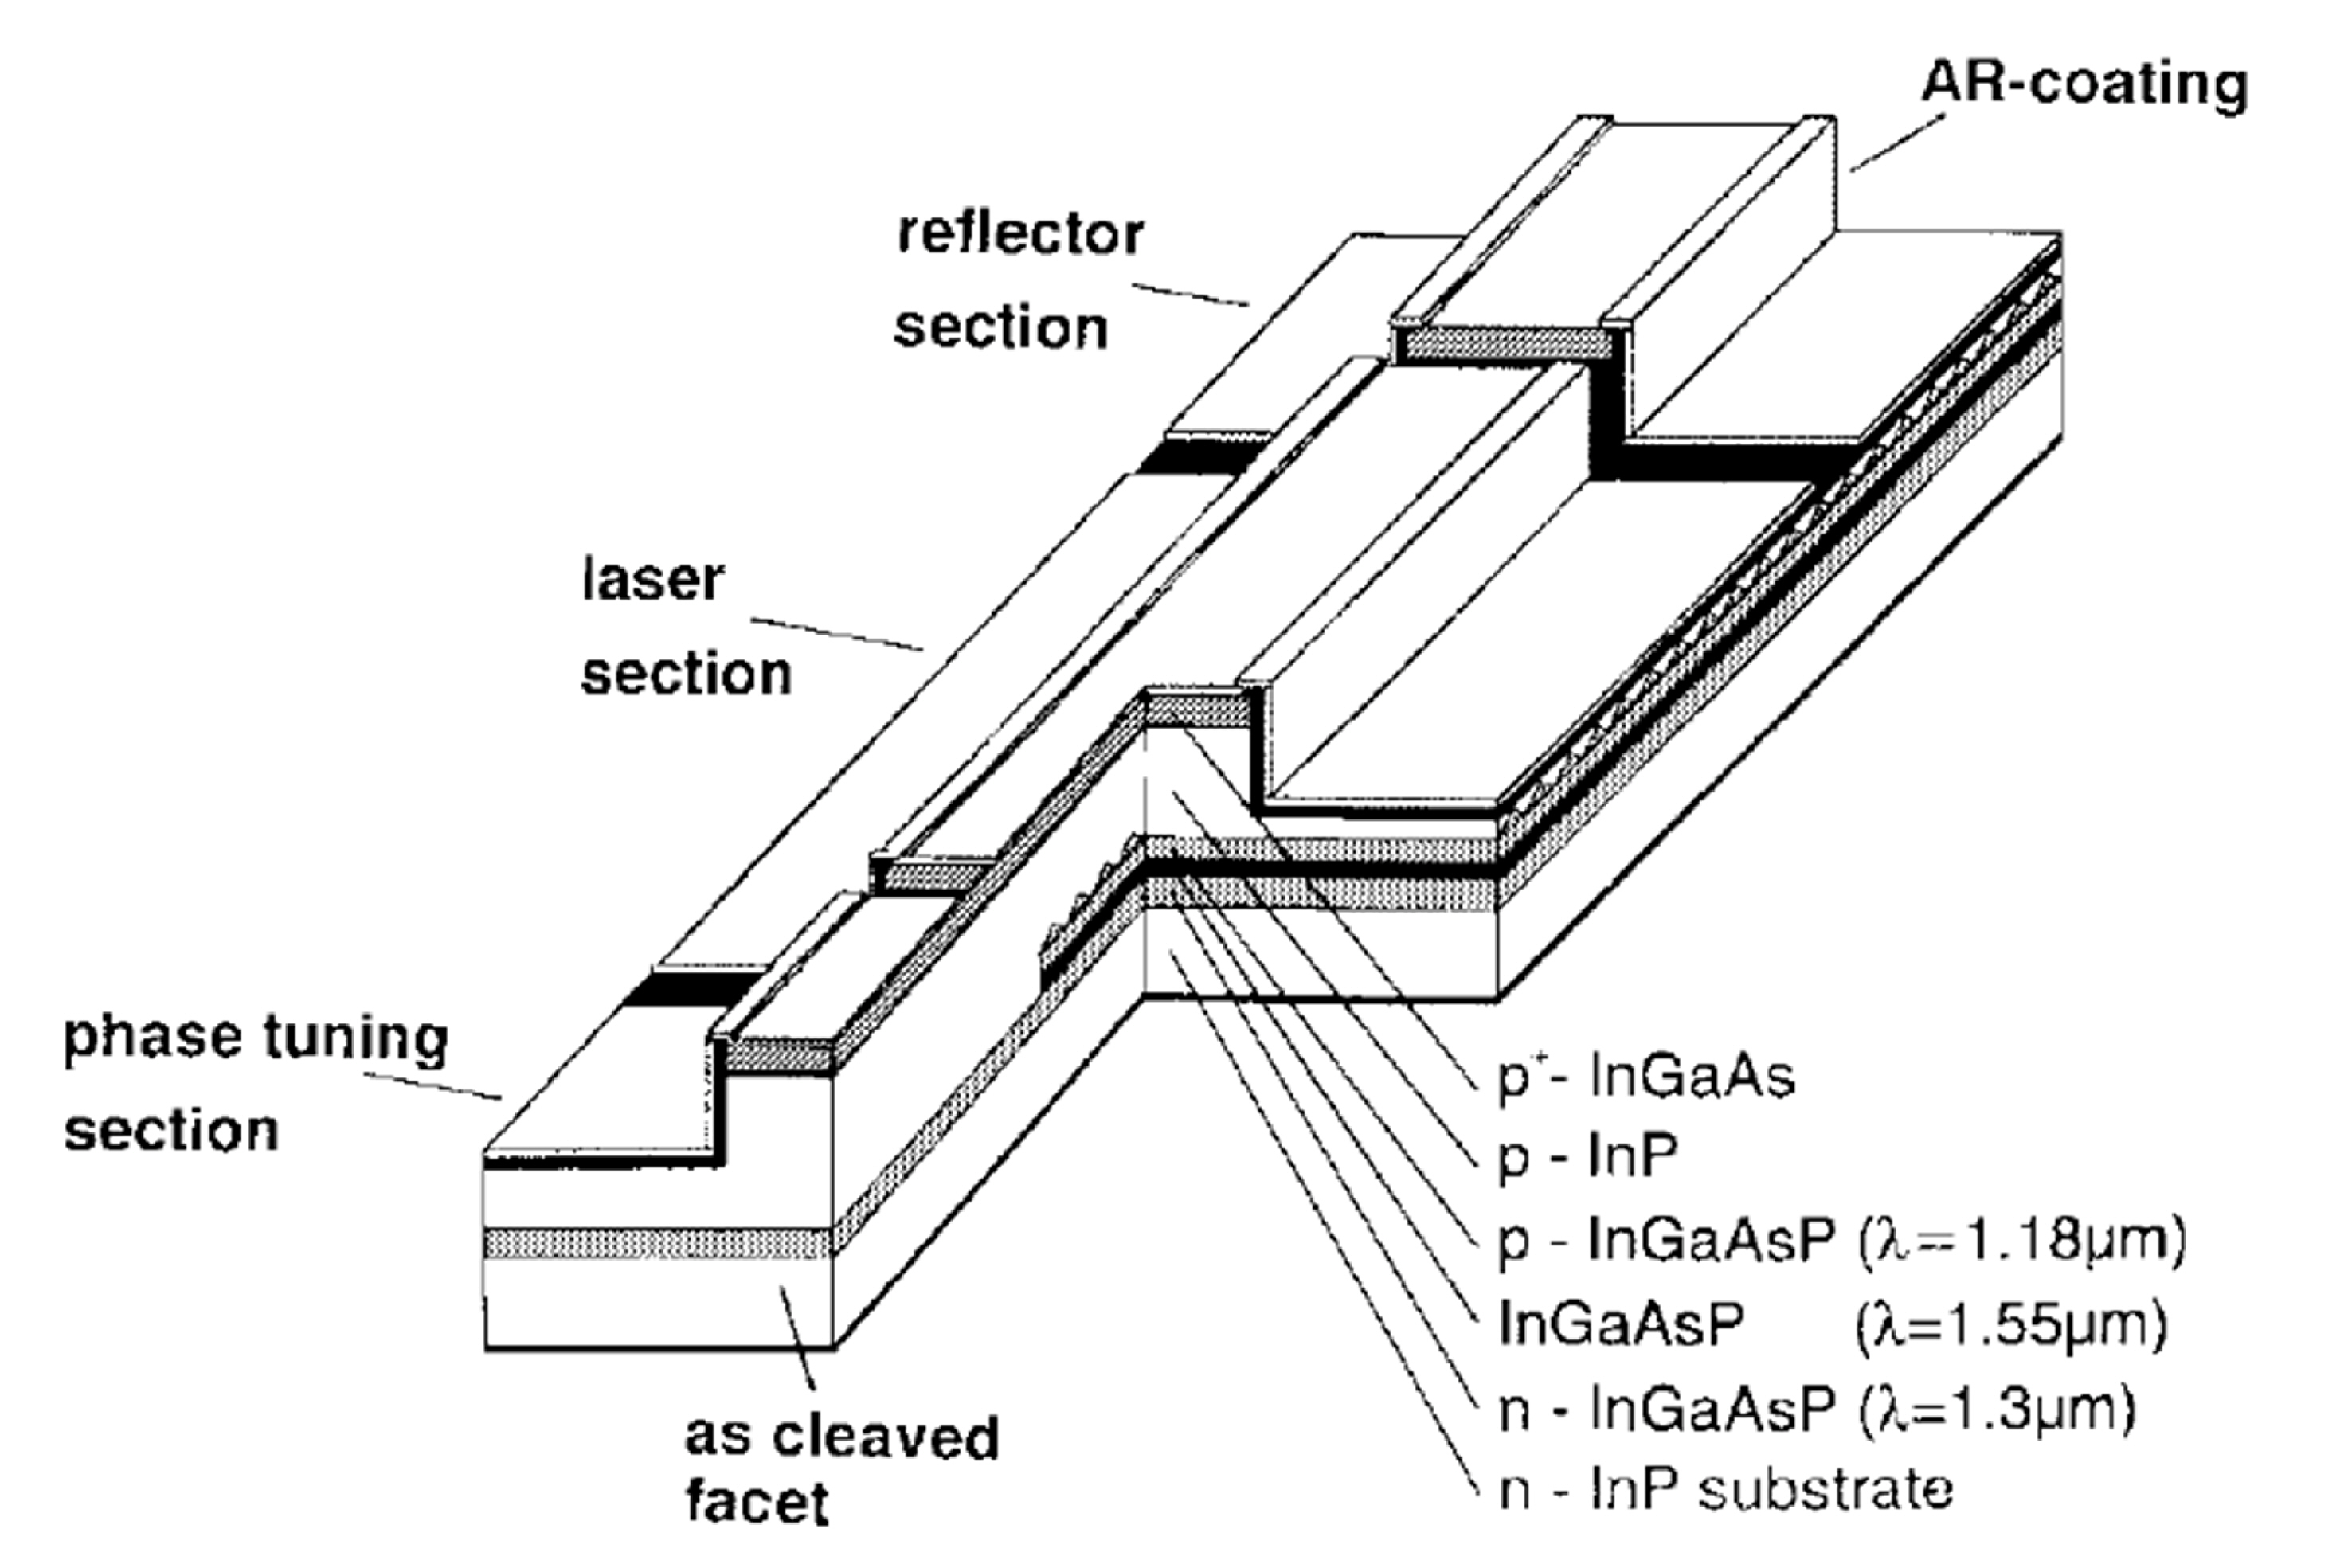
\includegraphics[width=14cm]{./Pictures/laser_twosectiondfb.jpg}
	\captionsetup{justification=centering}
	\caption{两段式DFB激光器\cite{sartorius1997dispersive}}
	\label{laser_twosectiondfb}
\end{figure}
\end{comment}

\section{自脉冲激光器的原理}
对于两段式DFB激光器来说,自脉冲形成的原理有如下三种\cite{sartorius1997dispersive}:

\begin{figure}[htb]
	\centering
	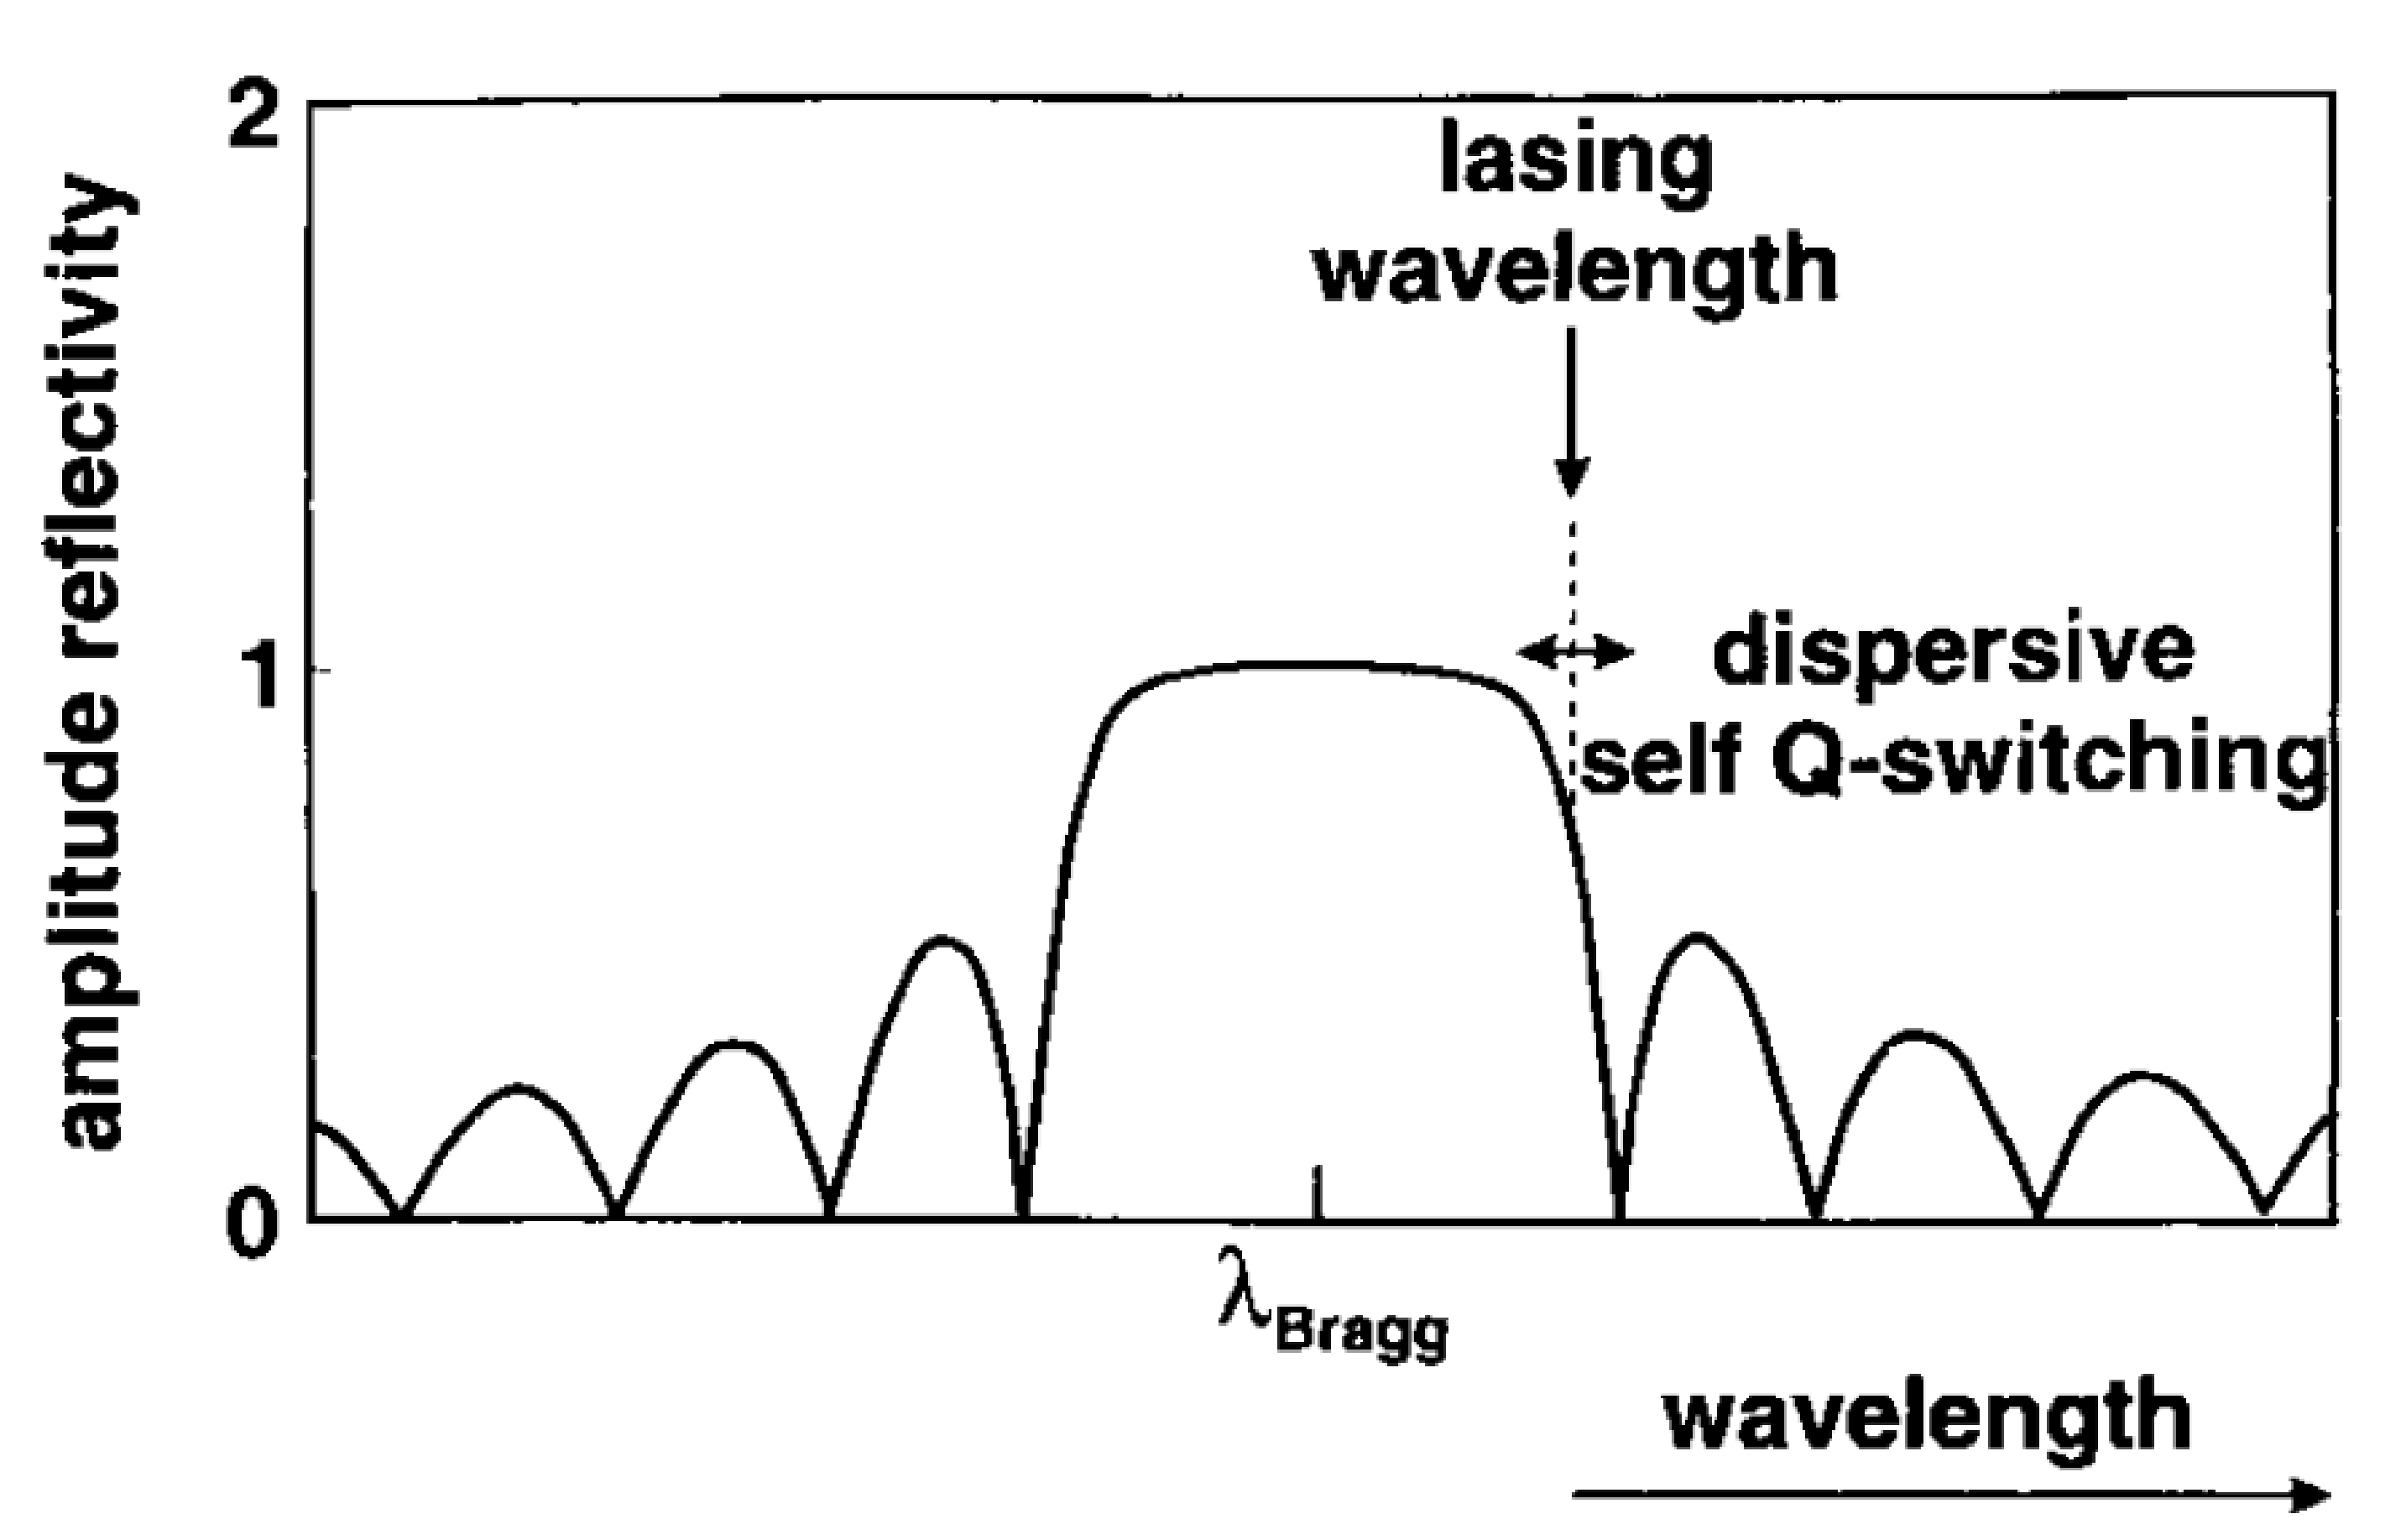
\includegraphics[width=12cm]{./Pictures/laser_selfQswitching.jpg}
	\captionsetup{justification=centering}
	\caption{色散自Q开关脉冲激光器的原理示意图\cite{sartorius1997dispersive}}
	\label{laser_selfQswitching}
\end{figure}

第一种是色散自调Q开关(dispersive self-Q-switching)产生自脉冲。其原理如图\ref{laser_selfQswitching}所示,其中双段式DFB激光器中的一段泵浦电流刚好使其工作在透明区域,即使其既没有增益,也没有损耗。在这种泵浦情况下,这段区域作为反射镜,需要利用的就是这个反射镜陡峭的反射谱。另一段DFB激光器的泵浦电流比较大,使其处于激发状态,且其发射波长刚好位于反射镜的右边的斜坡上。这样一来,这段激光器的阈值就会跟激射波长非常相关。当激光器处于激发状态时,载流子浓度下降,材料折射率上升,激光器的谐振波长就会往长波方向漂移,此时反射镜提供的反射率就会下降,激光器的阈值上升,激光不再出射;相反的,当激光不再出射,载流子浓度又开始上升,材料的折射率又会下降,使得谐振波长又往短波方向漂移,反射镜提供的反射率又会上升,激光器的阈值下降,激光又可以出射,如此周而往复,就形成了自脉冲的激光器。Bandelow等人\cite{bandelow1993theory}以单模为基础,利用传输波方程对该种类型的自脉冲激光器进行了研究。Marcenac等人\cite{marcenac1994distinction}则是用时域模型研究了类似的结构,都确认了该类型的自脉冲产生原因。总结起来,该种类型的自脉冲激光器有如下特征:

\begin{enumerate}
	\item 
	该种类型的自脉冲激光器都是单模的。
	\item 
	两段DFB激光器泵浦电流相差比较大。
	\item 
	自脉冲频率可以达到10GHz以上。
\end{enumerate}

第二种是空间烧孔效应产生自脉冲。当一个激光脉冲处于上升沿过程中,该模式的增益可能会由于空间烧孔效应下降,会出现跳模现象。当增益恢复之后,模式又会变回原来的模式,这个过程重复进行,就会出现自脉冲的现象。Lowery等人\cite{lowery1994improving}也观察到了自脉冲现象,他们将其归因于稳定的对称模式和不稳定的非对称模式之间由于空间烧孔效应引起的跳模。Phelan等人则认为除了空间烧孔效应,在多段DFB激光器中,载流子的互换也是产生自脉冲的原因之一。总结一下,对于空间烧孔效应引起的自脉冲激光器,有如下特征:

\begin{enumerate}
	\item 
	该种类型的自脉冲激光器都是多模的。
	\item 
	自脉冲频率一般小于5GHz。
\end{enumerate}

第三种是利用拍频产生自脉冲。这种机制由Wenzel等人\cite{wenzel1996mechanisms}提出。如果激光器的每一段都给予较高的泵浦电流,每一段都能产生一个激射波长,当这两个波长不一样时,就会出现拍频效应,拍频的频率正好是两束激光的频率之差,但这与两束不同的波长的激光相互干涉不一样,其中还包括了两段激光器之间光子与电子的互相耦合。这类自脉冲激光器的特征如下:

\begin{enumerate}
	\item 
	该种类型的自脉冲激光器都是多模的。
	\item 
	两段DFB激光器泵浦电流都比较大。
	\item 
	自脉冲频率可以达到100GHz以上。
\end{enumerate}

\section{硅基III-V混合集成技术}
如第一章所述,SOI平台上可以实现各种性能优异的无源器件,但是由于其为间接带隙材料,虽然科研人员在这个方向做了很多努力\cite{wirths2015lasing},要在其上制作电泵浦的激光器仍然困难重重。因此,人们非常希望能够将III-V材料和SOI结合来实现硅上的光源,这种方法可以同时利用硅和III-V材料各自的特点,从而可以在硅基平台上制作更加丰富的器件。

由于III-V材料与Si之间的晶格不匹配度达到8.1\%,在Si上直接外延生长会产生较多缺陷,故无法完美长出大面积的III-V外延层。虽然在第一章的介绍中已经介绍可以通过在Si上引入缓冲层或者限制缺陷扩展的结构,局部能够生长没有缺陷的外延层,实现了光泵浦激光器\cite{wang2015room},但是距离实现电泵浦激光器差距还很远。因此,现阶段研究人员主要采用键合的方式将III-V材料与SOI混合集成,实现在SOI上的电泵浦激光器,高速调制器、探测器和半导体光放大器\cite{liang2010hybrid,roelkens2010iii,liang2010recent,duan2014hybrid}。

\begin{figure}[htb]
	\centering
	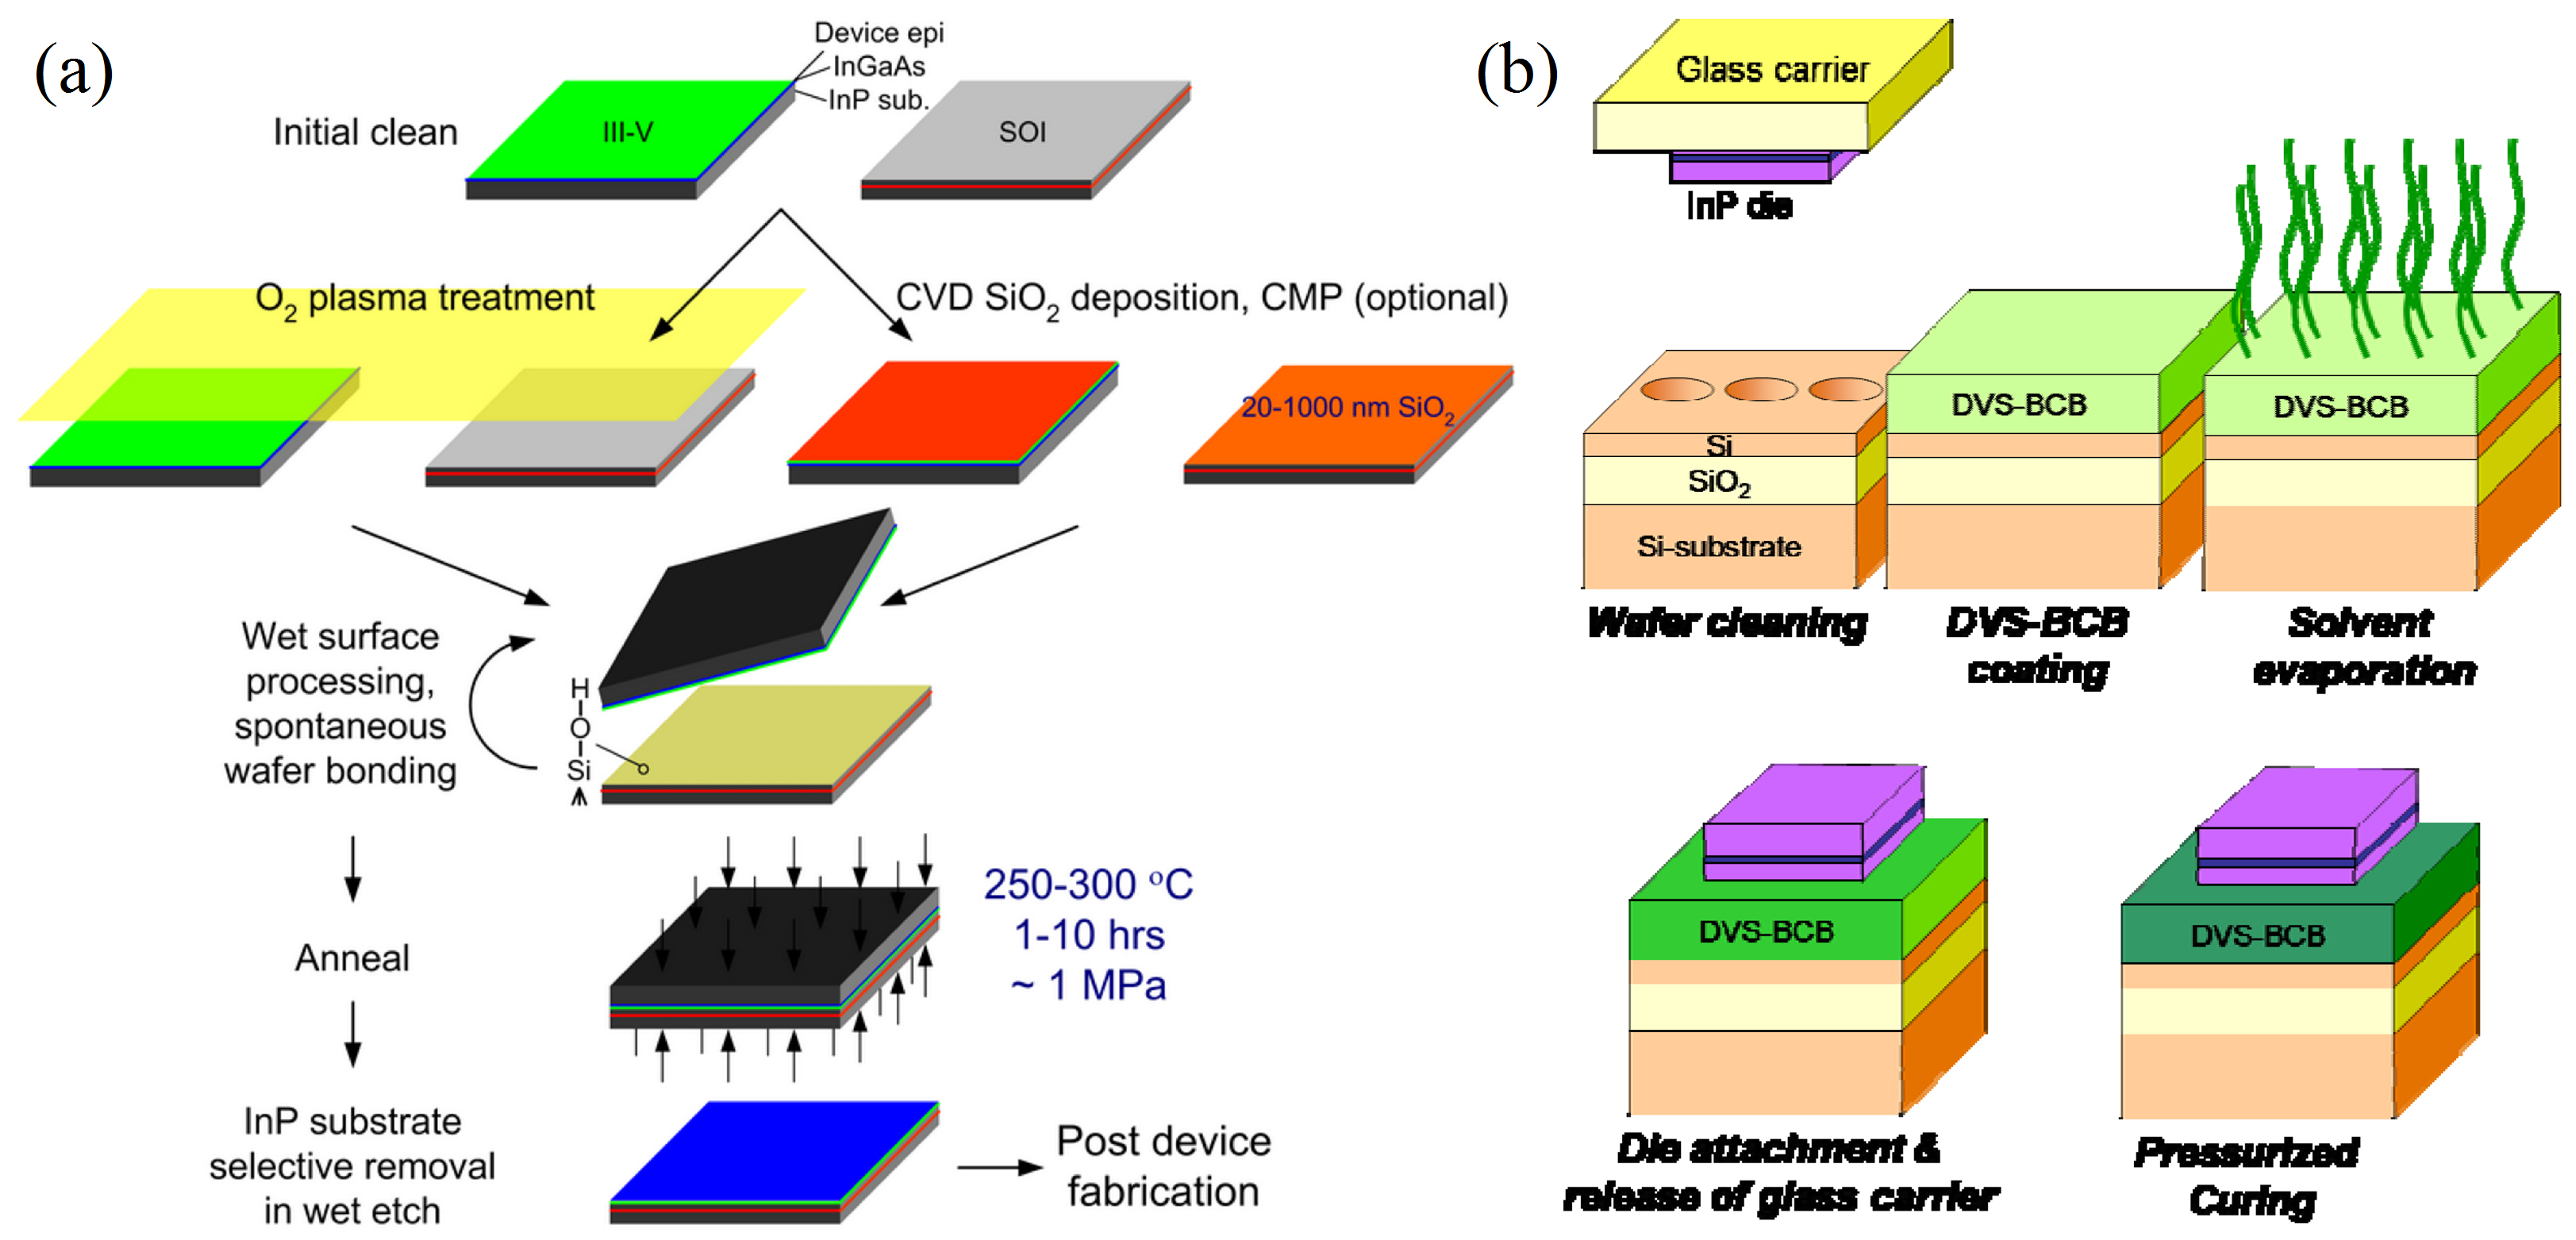
\includegraphics[width=14cm]{./Pictures/laser_bonding.jpg}
	\captionsetup{justification=centering}
	\caption{(a)III-V和SOI直接键合工艺流程示意图\cite{liang2010hybrid};(b)III-V和SOI粘贴键合工艺流程示意图\cite{liang2010hybrid}}
	\label{laser_bonding}
\end{figure}

目前,有两种比较常用的键合方式。一种是III-V芯片和SOI芯片通过O\SB{2}等离子体表面处理或者沉积SiO\SB{2}利用共价键直接键合的方式,具体工艺流程示意图如图\ref{laser_bonding}(a)所示。首先用BOE溶液去除InP芯片和SOI芯片表面的原生氧化层,获得干净疏水的表面。之后可以用O\SB{2}等离子体处理表面,使其产生约15 $nm$的等离子体氧化层,此时表面将变得非常光滑(RMS < 0.5 $nm$)且处于活化的状态。该过程中,O\SB{2}等离子体还起到了清洁晶片表面的作用,可以有效地去除表面的有机物。然后将InP芯片与SOI芯片贴合,在250~\~{}300 $^{\circ}$C、1 $MPa$的压力下进行退火处理,就可以将两者键合到一起。这种方法最早由瑞典的乌普萨拉大学的研究人员提出\cite{pasquariello2002plasma},后由美国加州大学圣塔芭芭拉分校(UCSB)的研究人员进一步优化\cite{liang2010hybrid},解决了键合表面会产生气体的问题。对于SiO\SB{2}共价键直接键合的方式,在第一步清洗完InP芯片与SOI芯片之后,在InP芯片表面通过PECVD长一层SiO\SB{2},在SOI芯片表面通过热氧长一层SiO\SB{2},之后通过化学机械腐蚀(chemical mechanical polishing, CMP)将表面的粗糙度下降到小于1 $nm$。然后可以通过稀释的标准RCA-1溶液在75 $^{\circ}$C下清洗10 $min$在表面形成Si-OH钝化层。之后的步骤则与用O\SB{2}等离子体处理表面直接建合法一样,通过贴合,加压退火,就可以将InP芯片与SOI芯片键合到一起。退火过程中发生的反应如公式\ref{bonding_1}和\ref{bonding_2}所示\cite{liang2010hybrid},其中M代表高电负性的金属(比如In, P):

\begin{equation}
\label{bonding_1}
\rm \ce{Si-OH} + \ce{M-OH} \rightarrow \ce{Si-O-M} +HOH(g)
\end{equation}

\begin{equation}
\label{bonding_2}
\rm Si + 2H_{2}O \rightarrow SiO_2 +2H_2(g)
\end{equation}

另一种键合的方式是III-V芯片和SOI芯片通过粘贴键合,其具体工艺流程示意图如图\ref{laser_bonding}(b)所示。首先用标准清洗溶液SC1(NH\SB{4}OH:H\SB{2}O\SB{2}:H\SB{2}O混合溶液)清洗SOI芯片,去除其表面的颗粒物并使其变成亲水性。对于III-V芯片,则是通过使用HCl和H\SB{2}SO\SB{4}:3H\SB{2}O\SB{2}:H\SB{2}O溶液分别去除InP和InGaAsP牺牲层来达到清洗的目的。将SOI芯片与III-V芯片清洗好之后,先在SOI芯片上旋涂一层增粘剂(AP-3000, Dow Chemicals),然后旋涂用来键合的粘贴剂。可以充当粘合剂的材料很多,比如PMMA,SU-8等,但是DVS-BCB(divinylsiloxane bis benzocyclobutene)相比其他材料,有更好的粘贴强度、热稳定性和抗腐蚀性能,其唯一的缺点只有热导率较低,故选择将其作为粘合剂材料。基于BCB的键合方法,主要由根特大学的研究人员开发\cite{roelkens2010iii}。旋涂BCB之后,将SOI芯片放于150~$^{\circ}$C的热板上烘烤1~$min$以去除BCB中的稀释用的溶剂——均三甲苯(mesitylene),这一步非常重要,否则容易在键合界面产生气泡。之后将III-V芯片有源层朝下倒扣到SOI芯片上,最后放入键合机中进行真空加压烘烤,烘烤温度为250~$^{\circ}$C。烘烤过程中,BCB单体会发生狄尔斯-阿尔德反应(Diels-Alder reaction)形成三维网状结构,反应示意图如图\ref{laser_bcb}所示。反应过程中无副产物生成,所以在键合界面不会生成气泡。

\begin{figure}[htb]
	\centering
	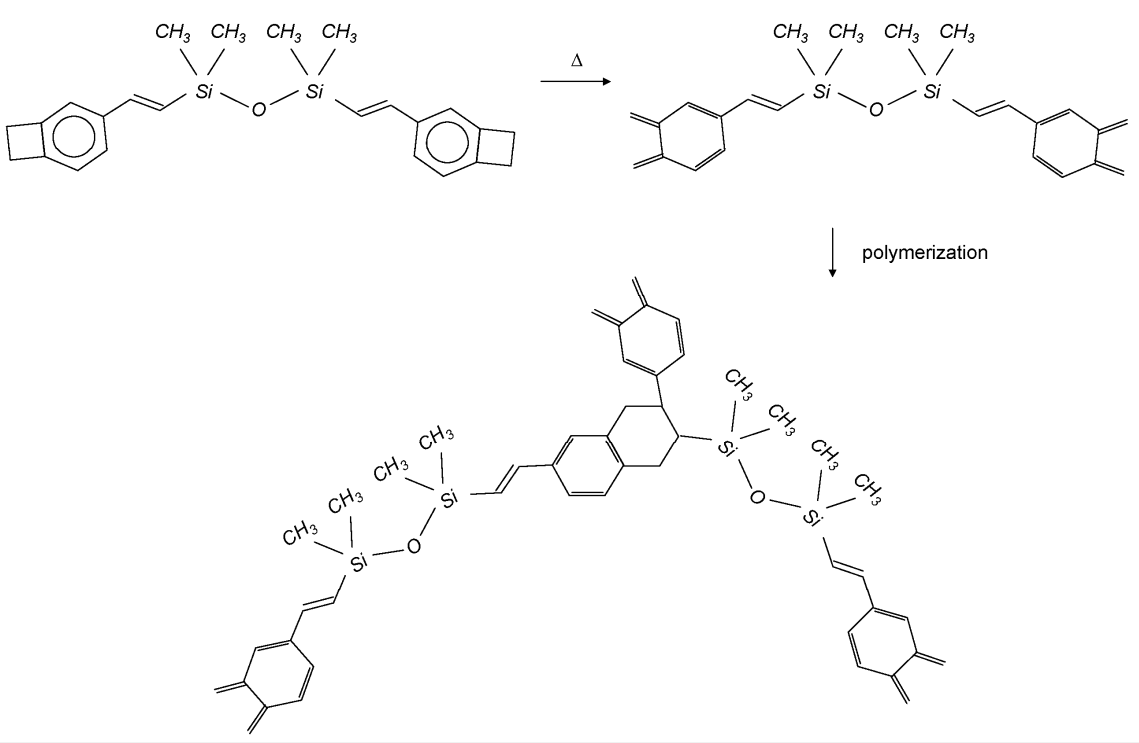
\includegraphics[width=11cm]{./Pictures/laser_bcb.png}
	\captionsetup{justification=centering}
	\caption{DVS-BCB单体聚合反应}
	\label{laser_bcb}
\end{figure}

虽然通过直接键合的方式,III-V芯片和SOI芯片之间的距离可以更近,更加方便光的耦合,但是其对III-V芯片和SOI芯片的表面粗糙度和洁净度要求非常高,工艺较为复杂。而通过BCB键合的方式,由于有中间层BCB的存在,降低了对III-V芯片和SOI芯片表面粗糙度和洁净度的要求\cite{roelkens2007heterogeneous},而且,通过将BCB稀释,也可以获得厚度小于100~$nm$的键合层,实现III-V波导和SOI波导之间光的耦合,故本文采用BCB粘贴键合的方式来制作混合集成的DFB激光器。

\section{器件的设计}

我们采用双段式DFB激光器的结构,通过拍频的方式实现自脉冲信号的产生,因为DFB激光器的单模性能较好,边摸抑制比高,故可以得到较为纯净的自脉冲信号。本文使用的多量子阱外延片的结构如表\ref{laser_material}所示,由台湾Landmark公司加工生产。

\begin{table}[htb]
	\zihao{5}
	\captionsetup{justification=centering}
	\caption{III-V外延片的材料参数}
	\label{laser_material}
	\centering
	\begin{tabular}[t]{|llll|}
		\hline
		\textbf{名称} & \textbf{材料组分} & \textbf{掺杂浓度 ($\pmb{cm^{-3}}$)} & \textbf{厚度($\pmb{nm}$)} \\
		\hline
		Sacrificial & InP & - &  200 \\
		\hline 
		Sacrificial & InGaAs & - &  200 \\
		\hline
		N cladding & InP & 1.00E18 & 190 \\
		\hline
		SCH & InGaAsP(Q1.17) & - & 100 \\
		\hline
		MQW well$\times$6 & InGaAsP(Q1.55) & - & 7 \\
		\hline
		MQW barrier$\times$7 & InGaAsP(Q1.17) & - & 9 \\
		\hline
		SCH & InGaAsP(Q1.17) & - & 100 \\
		\hline
		P cladding & InP & 5.00E17 & 500 \\
		\hline 
		P cladding & InP & 5.00E17->2.00E18 & 1000\\
		\hline
		Transition & InGaAsP(Q1.2) & >3.00E18 & 10\\
		\hline
		Transition & InGaAsP(Q1.4) & >3.00E18 & 10\\
		\hline
		P contact & InGaAsP & >1.5E19 & 200 \\
		\hline
		Sacrificial & InP & - & 200 \\
		\hline
		Stop etch & InGaAs & - & 200 \\
		\hline
		Substrate & InP & - & -\\
		\hline
	\end{tabular}
\end{table}

该外延片的PL谱测试结果如图\ref{laser_PL}所示,可以看到该外延片的光致荧光谱中心波长在1544.9 $nm$,增益带宽为63.0 $nm$。

\begin{figure}[htb]
	\centering
	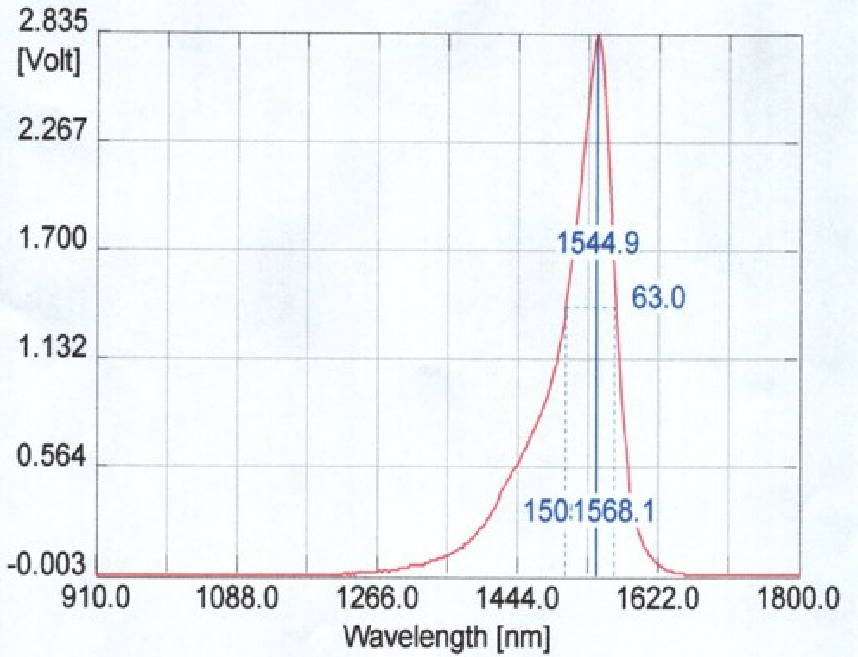
\includegraphics[width=10cm]{./Pictures/laser_PL.png}
	\captionsetup{justification=centering}
	\caption{表\ref{laser_material}所示的多量子阱外延片的光致荧光谱}
	\label{laser_PL}
\end{figure}

\begin{figure}[htb]
	\centering
	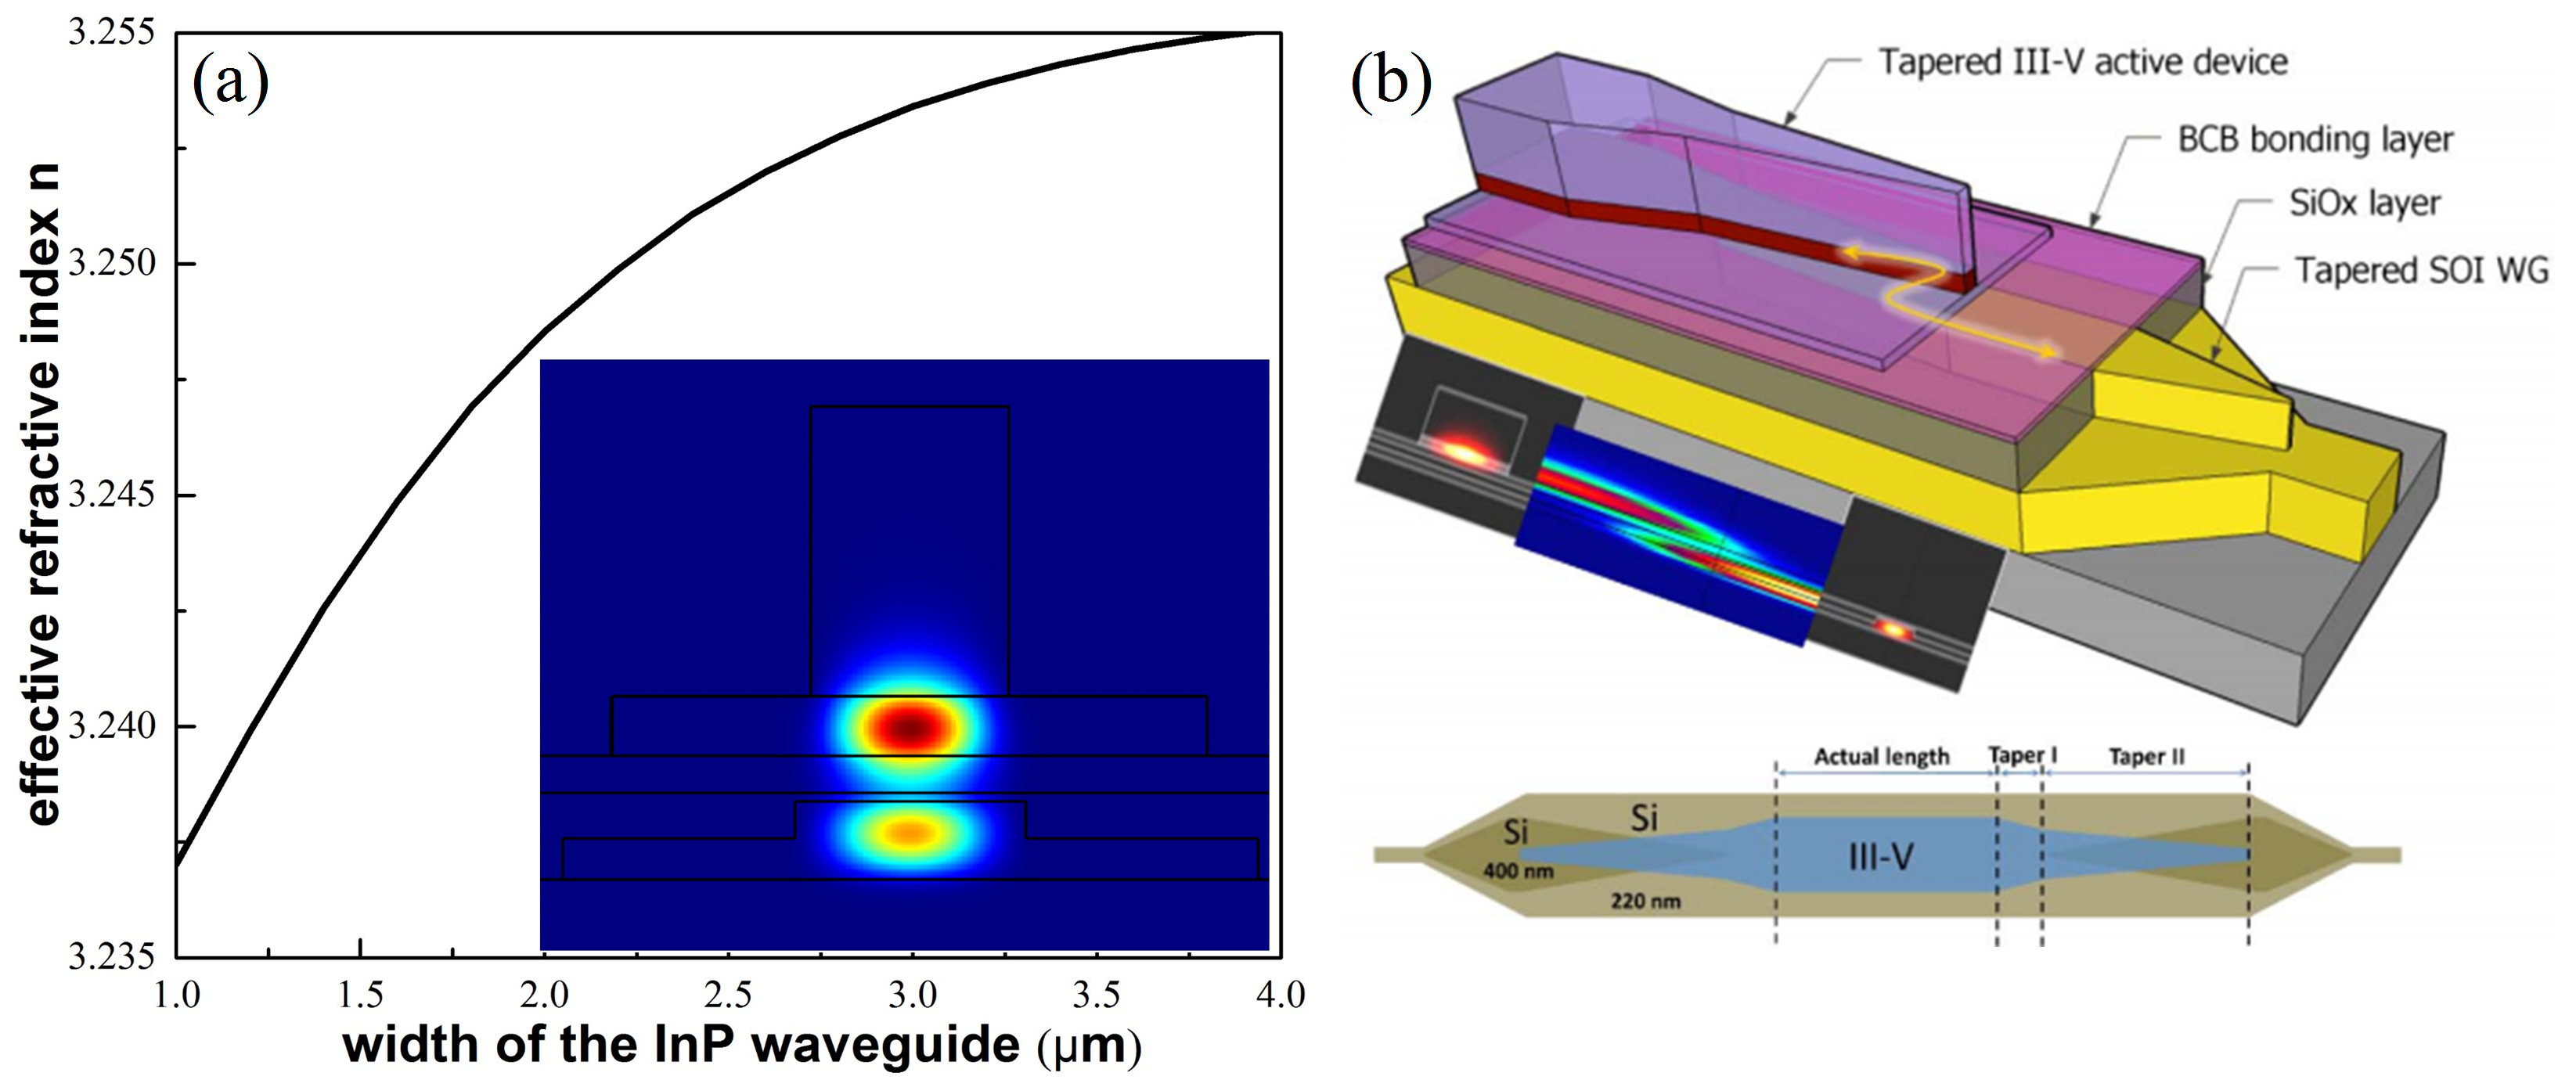
\includegraphics[width=14cm]{./Pictures/laser_modeandtaper.jpg}
	\captionsetup{justification=centering}
	\caption{(a)激光器的截面模式等效折射率随p-InP宽度变化图,插图为模式分布图;(b)两段式反向taper\cite{keyvaninia2013heterogeneously}}
	\label{laser_modeandtaper}
\end{figure}

III-V外延片中1.5 $\mu m$厚的P型InP层是为了让光传播模式远离高吸收的InGaAs层,减小III-V波导中的模式损耗。该多量子阱层由6层7~$nm$的InGaAsP势阱和7层9~$nm$的InGaAsP势垒组成。我们采用一阶光栅作为DFB激光器的光栅,将光栅制作在硅层厚度为400 $nm$的SOI芯片上,刻蚀深度为180 $nm$,周期$\Lambda$为246 $nm$,占空比为0.5,光栅宽度为3.5 $\mu m$,波导宽度为10.5 $\mu m$。III-V材料通过BCB与SOI键合,在光栅区域形成混合模式,部分能量在III-V材料中,部分能量在Si波导中。通过仿真得到如图\ref{laser_modeandtaper}(a)插图所示的截面模式图,该模式在量子阱中的限制因子为14.7\%,模式的限制因子越高,可以使激光器的阈值越低。激光器两边各通过一个反向锥形波导耦合器将光耦合到220~$nm$的硅波导中。锥形波导耦合器的结构用Keyvaninia等人采用的结构\cite{keyvaninia2013heterogeneously},如图\ref{laser_modeandtaper}(b)所示。该锥形波导耦合器分为两段且总长度为200 $\mu m$,第一段III-V波导从3~$\mu m$线性变到1~$\mu m$,长度为50~$\mu m$;第二段III-V波导从1~$\mu m$线性变化到600~$nm$,下面的脊型硅波导宽度从300~$nm$线性变化到2~$\mu m$,总长度为150~$\mu m$,该锥形波导耦合器可以实现高于90\%以上的耦合效率。

最后,我们设计的自脉冲DFB激光器如图\ref{laser_structure}所示,该激光器采用双段式设计,两边采用不一样的宽度是为了在同样的泵浦电流下,两段DFB激光器输出的波长错开一个阻带的宽度,从而可以同时用来研究色散自调Q开关和拍频产生自脉冲的现象。根据经验,该DFB激光器的阻带宽度约为4~\~{}5~$nm$左右,根据公式$2\Delta n_{eff}\Lambda = \Delta\lambda$计算得到$\Delta n_{eff}\approx 0.009$。根据\ref{laser_modeandtaper}(a)中等效折射率与p-InP波导宽度之间的关系,我们选取两段p-InP波导的宽度分别为2~$\mu m$和4~$\mu m$。p-InGaAs层在中间被刻蚀掉是为了进行电隔离,从而两段激光器可以注入不同的电流,倾斜的刻蚀可以尽量减少反射的光返回谐振腔内。产生的激光通过锥形波导耦合器耦合到硅波导,之后通过耦合光栅输出到光纤进行后续测试。

\begin{figure}[htb]
	\centering
	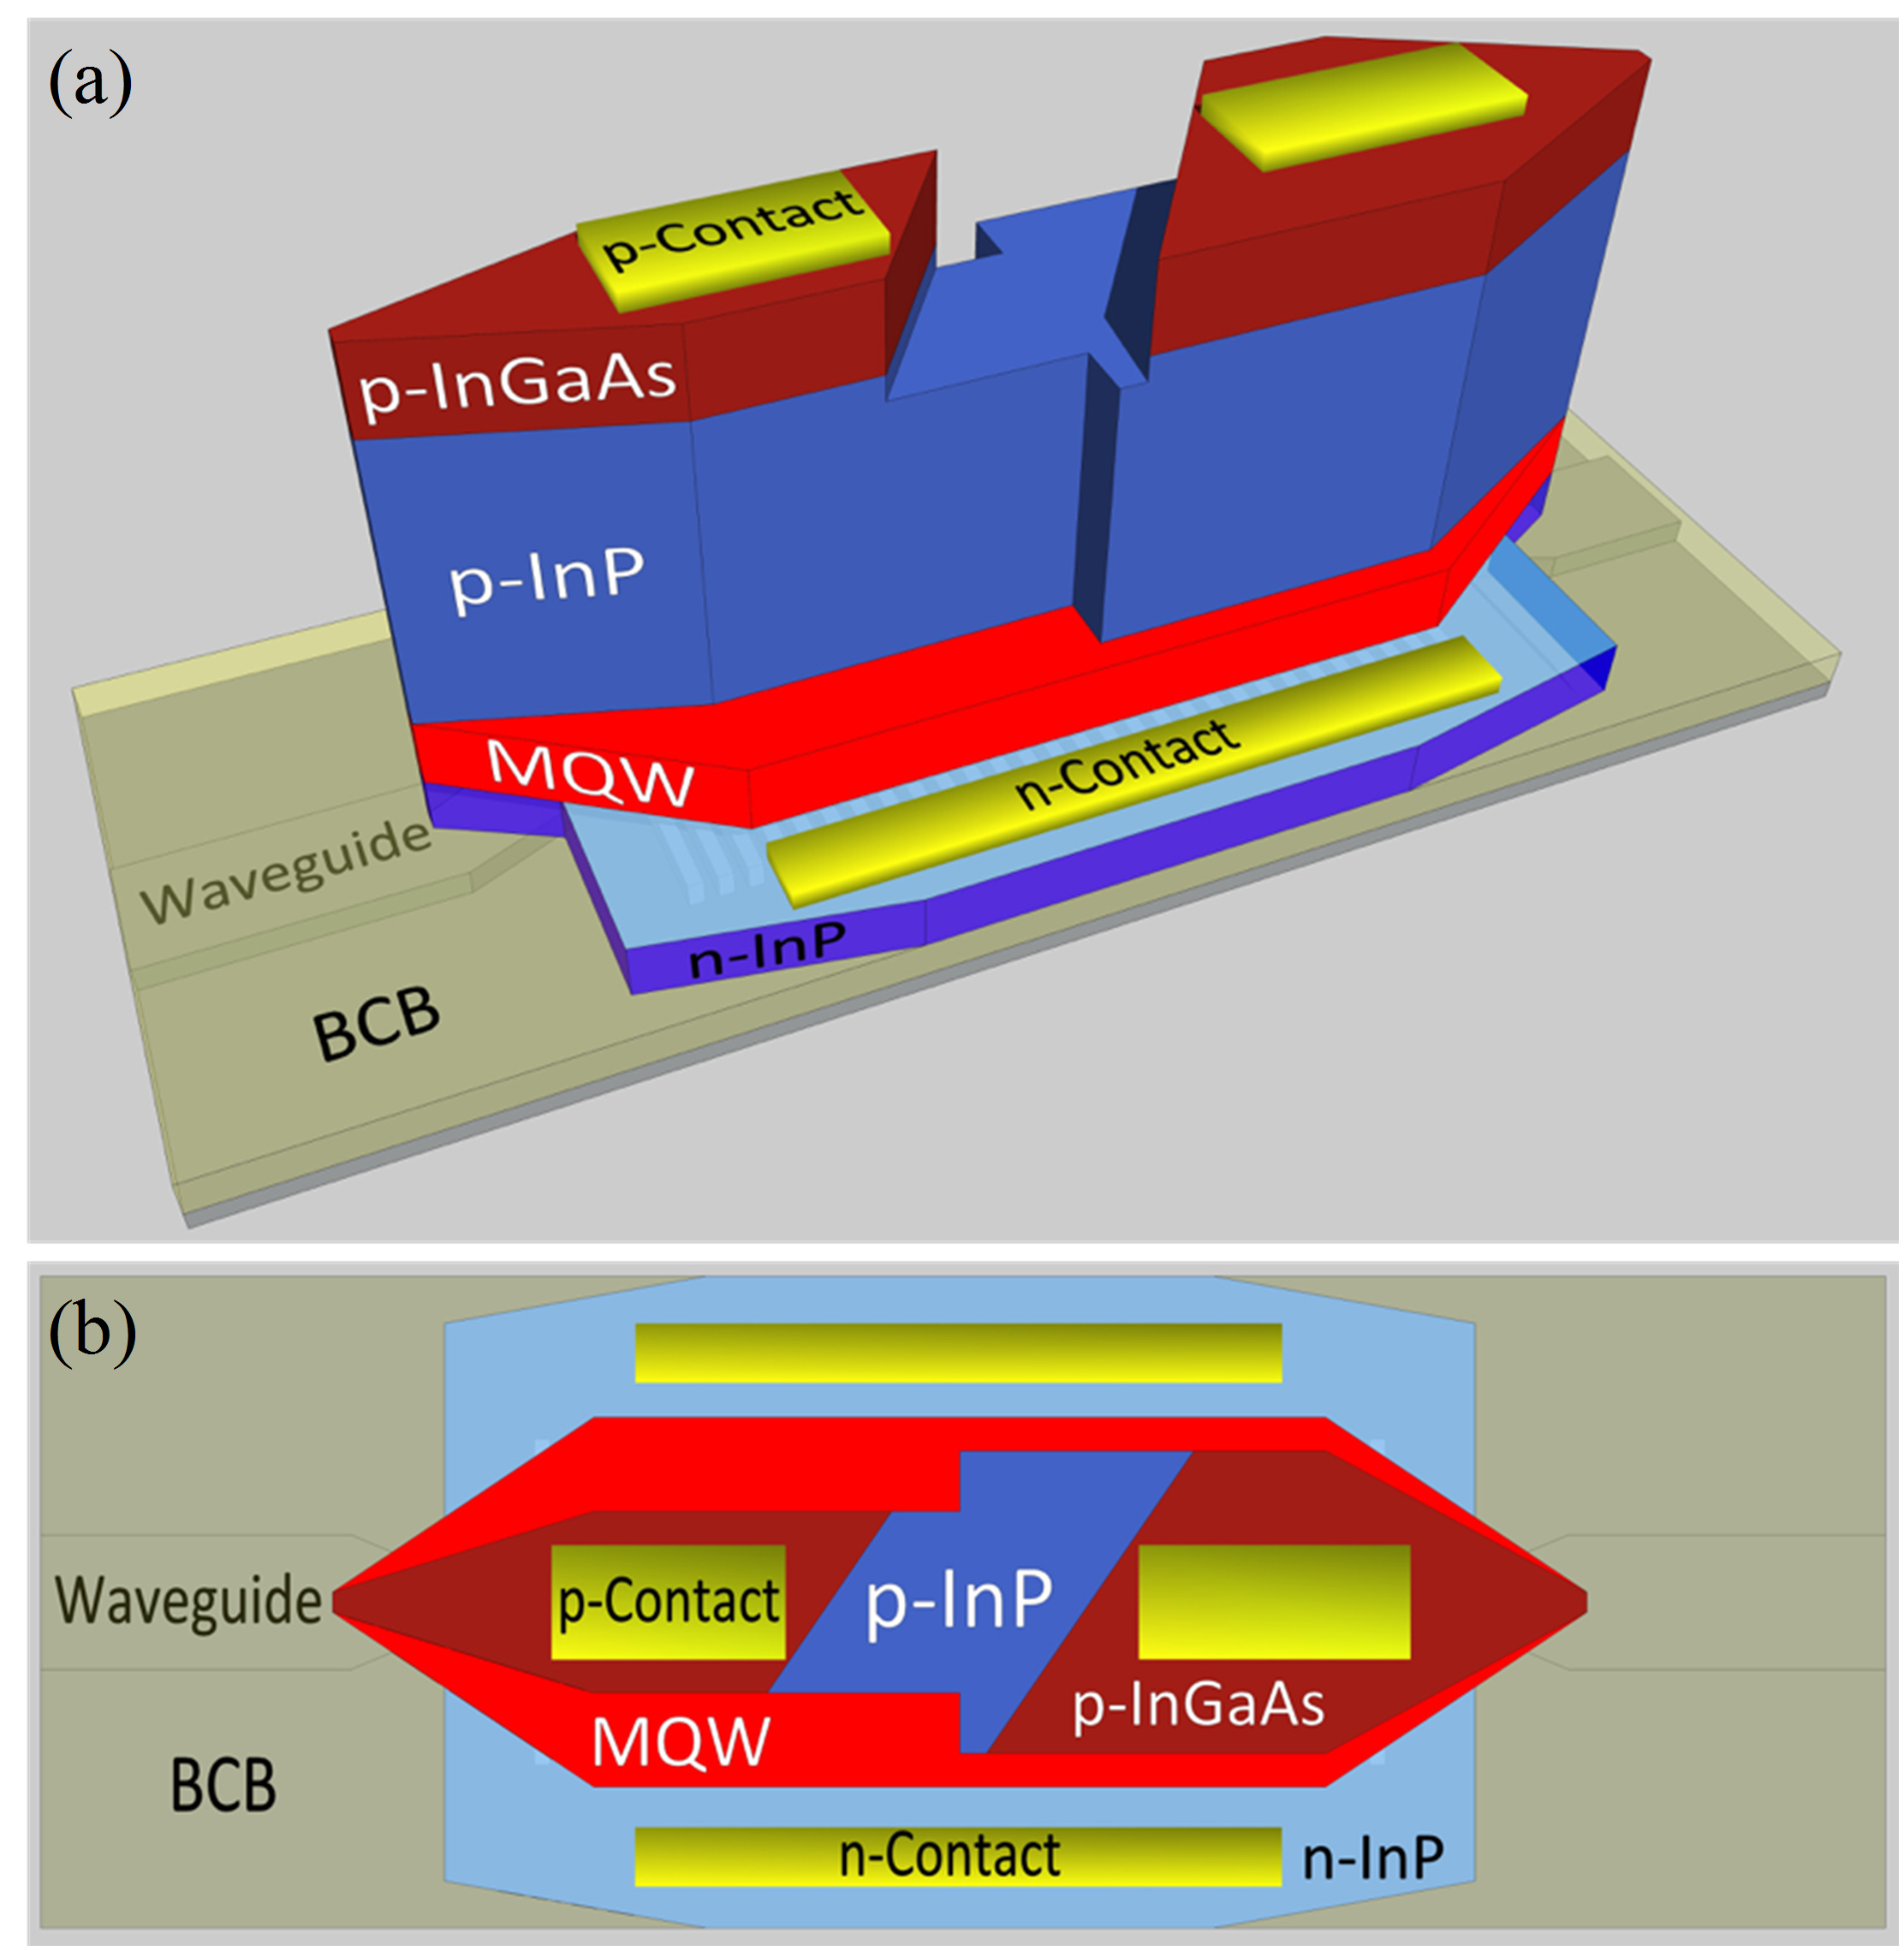
\includegraphics[width=12cm]{./Pictures/laser_structure.jpg}
	\captionsetup{justification=centering}
	\caption{双段式DFB激光器示意图,(a)~3D试图;(b)俯视图}
	\label{laser_structure}
\end{figure}

\section{制作工艺}

SOI芯片上的DFB光栅可以通过实验室电子束曝光之后使用ICP刻蚀完成或者委托半导体公司流片进行制作。用电子束曝光加ICP刻蚀的方法比较灵活,方便修改参数,加工周期短,但是波导损耗会较大且均一性较差。因为激光器对损耗相对比较敏感,实验室制作成功率不是特别高,如果采用EBL加工SOI芯片上的DFB光栅均一性无法保证。委托半导体公司进行流片,可以获得大量均一性好,损耗低的DFB一阶光栅,方便用来进行工艺摸索。我们委托Imec\cite{Imec}制作了SOI芯片上的DFB光栅。半导体公司流片时,会用100~$nm$左右的SiO\SB{2}进行表面平坦化处理,我们在进行键合时需要将该层去除,以增强硅波导与III-V波导之间的耦合。

下面介绍基于DVS-BCB粘贴键合的硅基混合集成DFB激光器制作工艺,主要分为两个部分。第一个部分是键合工艺;第二个部分是III-V波导与电极制作部分:
\begin{enumerate}[(1)]
	\item 
	从流片回来的SOI大晶圆上解理需要键合的芯片,为了方便操作,大小可以选取为2.5~$cm$~$\times$~2.5~$cm$,解理时需使所需要的DFB光栅处于芯片的中央位置,这样在键合时,III-V芯片位于SOI芯片的中央位置。解理时可以在表面旋涂一层光刻胶进行保护,防止解理产生的碎片划伤芯片表面。用丙酮、异丙醇清洗之后,再缓冲HF腐蚀液(buffered HF, BHF)去掉表面用于平坦化的SiO\SB{2}。
	\item 
	解理合适大小的III-V芯片,一般使其比SOI芯片上的DFB光栅区域边长大1~$mm$左右就已足够。用丙酮去除其表面用来保护的光刻胶,之后用HCl:H\SB{2}O=1:1的溶液去除InP牺牲层,再用食人鱼溶液H\SB{2}SO\SB{4}:H\SB{2}O\SB{2}:H\SB{2}O=1:1:18去除InGaAs牺牲层,可通过观察颜色来确定牺牲层是否去除干净。
	\item 
	为了增加III-V与BCB的粘附性,键合之前需要在III-V芯片上表面用PECVD长一层5~$nm$左右的SiO\SB{2}。
	\item 
	将SOI芯片与III-V芯片在150$^{\circ}$C热板上烘烤去水汽,然后在SOI芯片上旋涂BCB:均三甲苯(Mesatylane)=1:8的溶液,参数为500~rpm~5~$s$,3000~rpm~40~$s$。将匀好BCB的SOI芯片在150~$^{\circ}$C热板上烘烤10\~{}20~$min$,将溶剂均三甲苯挥发掉,防止键合时产生气泡。之后将热板调成20~$^{\circ}$C,当热板冷却到70~$^{\circ}$C时,将芯片取下,放于键合机的石英载玻片上准备键合。然后用镊子将III-V芯片倒扣到SOI芯片上,此步需要手工完成,并借助显微镜确定III-V芯片全部覆盖了SOI芯片上的DFB光栅。为了之后湿法腐蚀的III-V波导形成倒梯形的结构,使得模式可以更好的限制在多量子阱层中,III-V芯片的[011]晶向需要对准SOI芯片上的波导方向。
	\item 
	利用商用键合机S\.{U}SS MicroTec ELAN CB6L进行键合,由于该键合机适用于键合4英寸的芯片,而我们的芯片尺寸较小,因此我们需要将手工键合的芯片夹在两片4英寸的石英载玻片之间,如图\ref{laser_bonder}(a)所示。随后,我们将其放入键合机内进行键合,键合机会在真空环境下进行键合,这可以帮助将III-V芯片与SOI芯片之间的空气排除干净。键合机内的温度和压力变化曲线如图\ref{laser_bonder}(b)所示,当温度上升到150~$^{\circ}$C时,BCB还具有一定的流动性,这时加入200\~{}400~$KPa$的压力可以减小BCB的厚度,同时可以更好地填充III-V芯片与SOI芯片之间的缝隙,使得键合的强度更强。当温度高于180~$^{\circ}$C后,压力被撤去,以防BCB在高温玻璃化时产生较大的应力。键合完成后的芯片如图\ref{laser_bonder}(c)所示。
	\begin{figure}[htb]
		\centering
		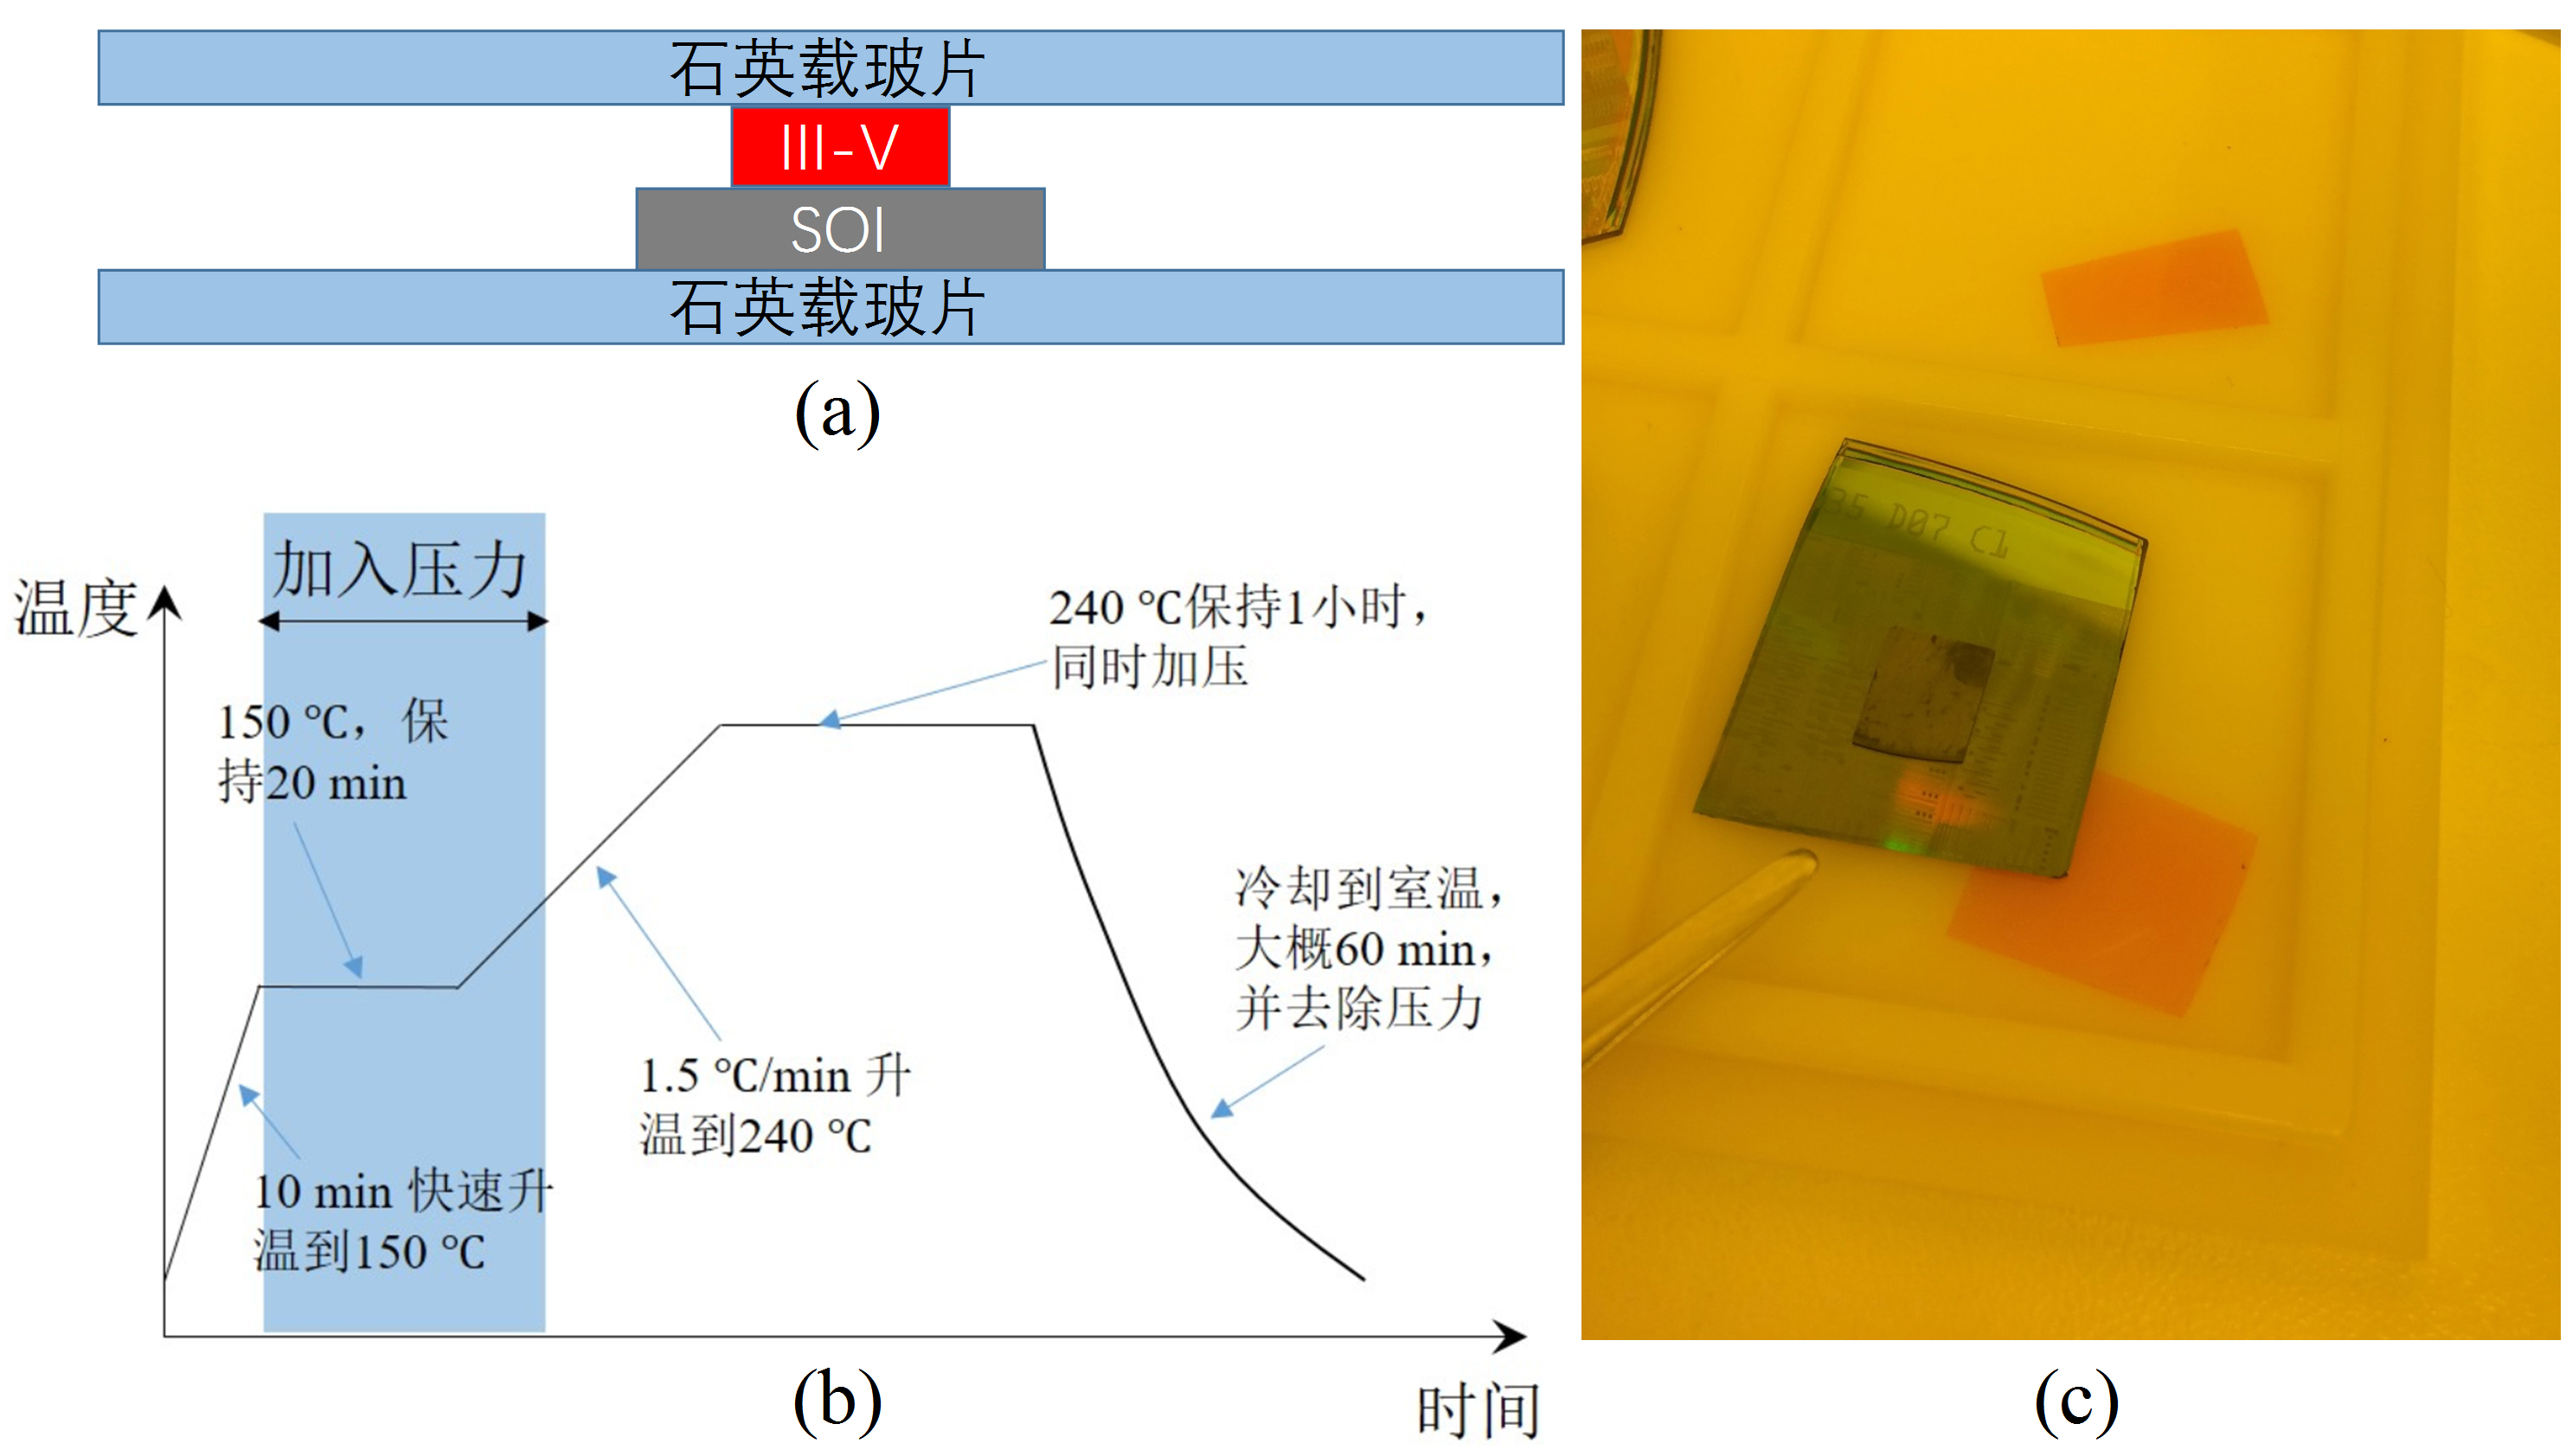
\includegraphics[width=15cm]{./Pictures/laser_bonder.jpg}
		\captionsetup{justification=centering}
		\caption{(a)夹在两片4英寸石英载玻片之间的SOI芯片和III-V芯片;(b)键合机键合过程中温度和压力随时间变化曲线;(c)键合完成后的芯片}
		\label{laser_bonder}
	\end{figure}
	\item 
	用HCL:H\SB{2}O=3:1的溶液加热到40~$^{\circ}$C去除III-V芯片的衬底InP,加热是为了加快去除衬底的速度。当不再有气泡产生时,说明衬底已经去除干净,总时间大约为15\~{}25~$min$。有时如果键合的质量不够好,去除衬底之后部分III-V芯片就会脱落,如图\ref{laser_sub_removal}(a)所示,这是由于去除衬底之后III-V芯片厚度只有2.615~$\mu m$,如有应力存在,较容易破裂。但如果掉落的面积不大,有的DFB光栅上依然有III-V芯片,则实验可以继续。\ref{laser_sub_removal}(b)所示为去除衬底过程中的侧向腐蚀现象,HCl通过边缘腐蚀InP,这可以通过在III-V芯片四周涂抹一层光刻胶解决,但是一般只要在解理III-V芯片时稍微留点余量,则问题并不大,可以看到侧向腐蚀最大处也不过400~$\mu m$不到。
	\begin{figure}[htb]
		\centering
		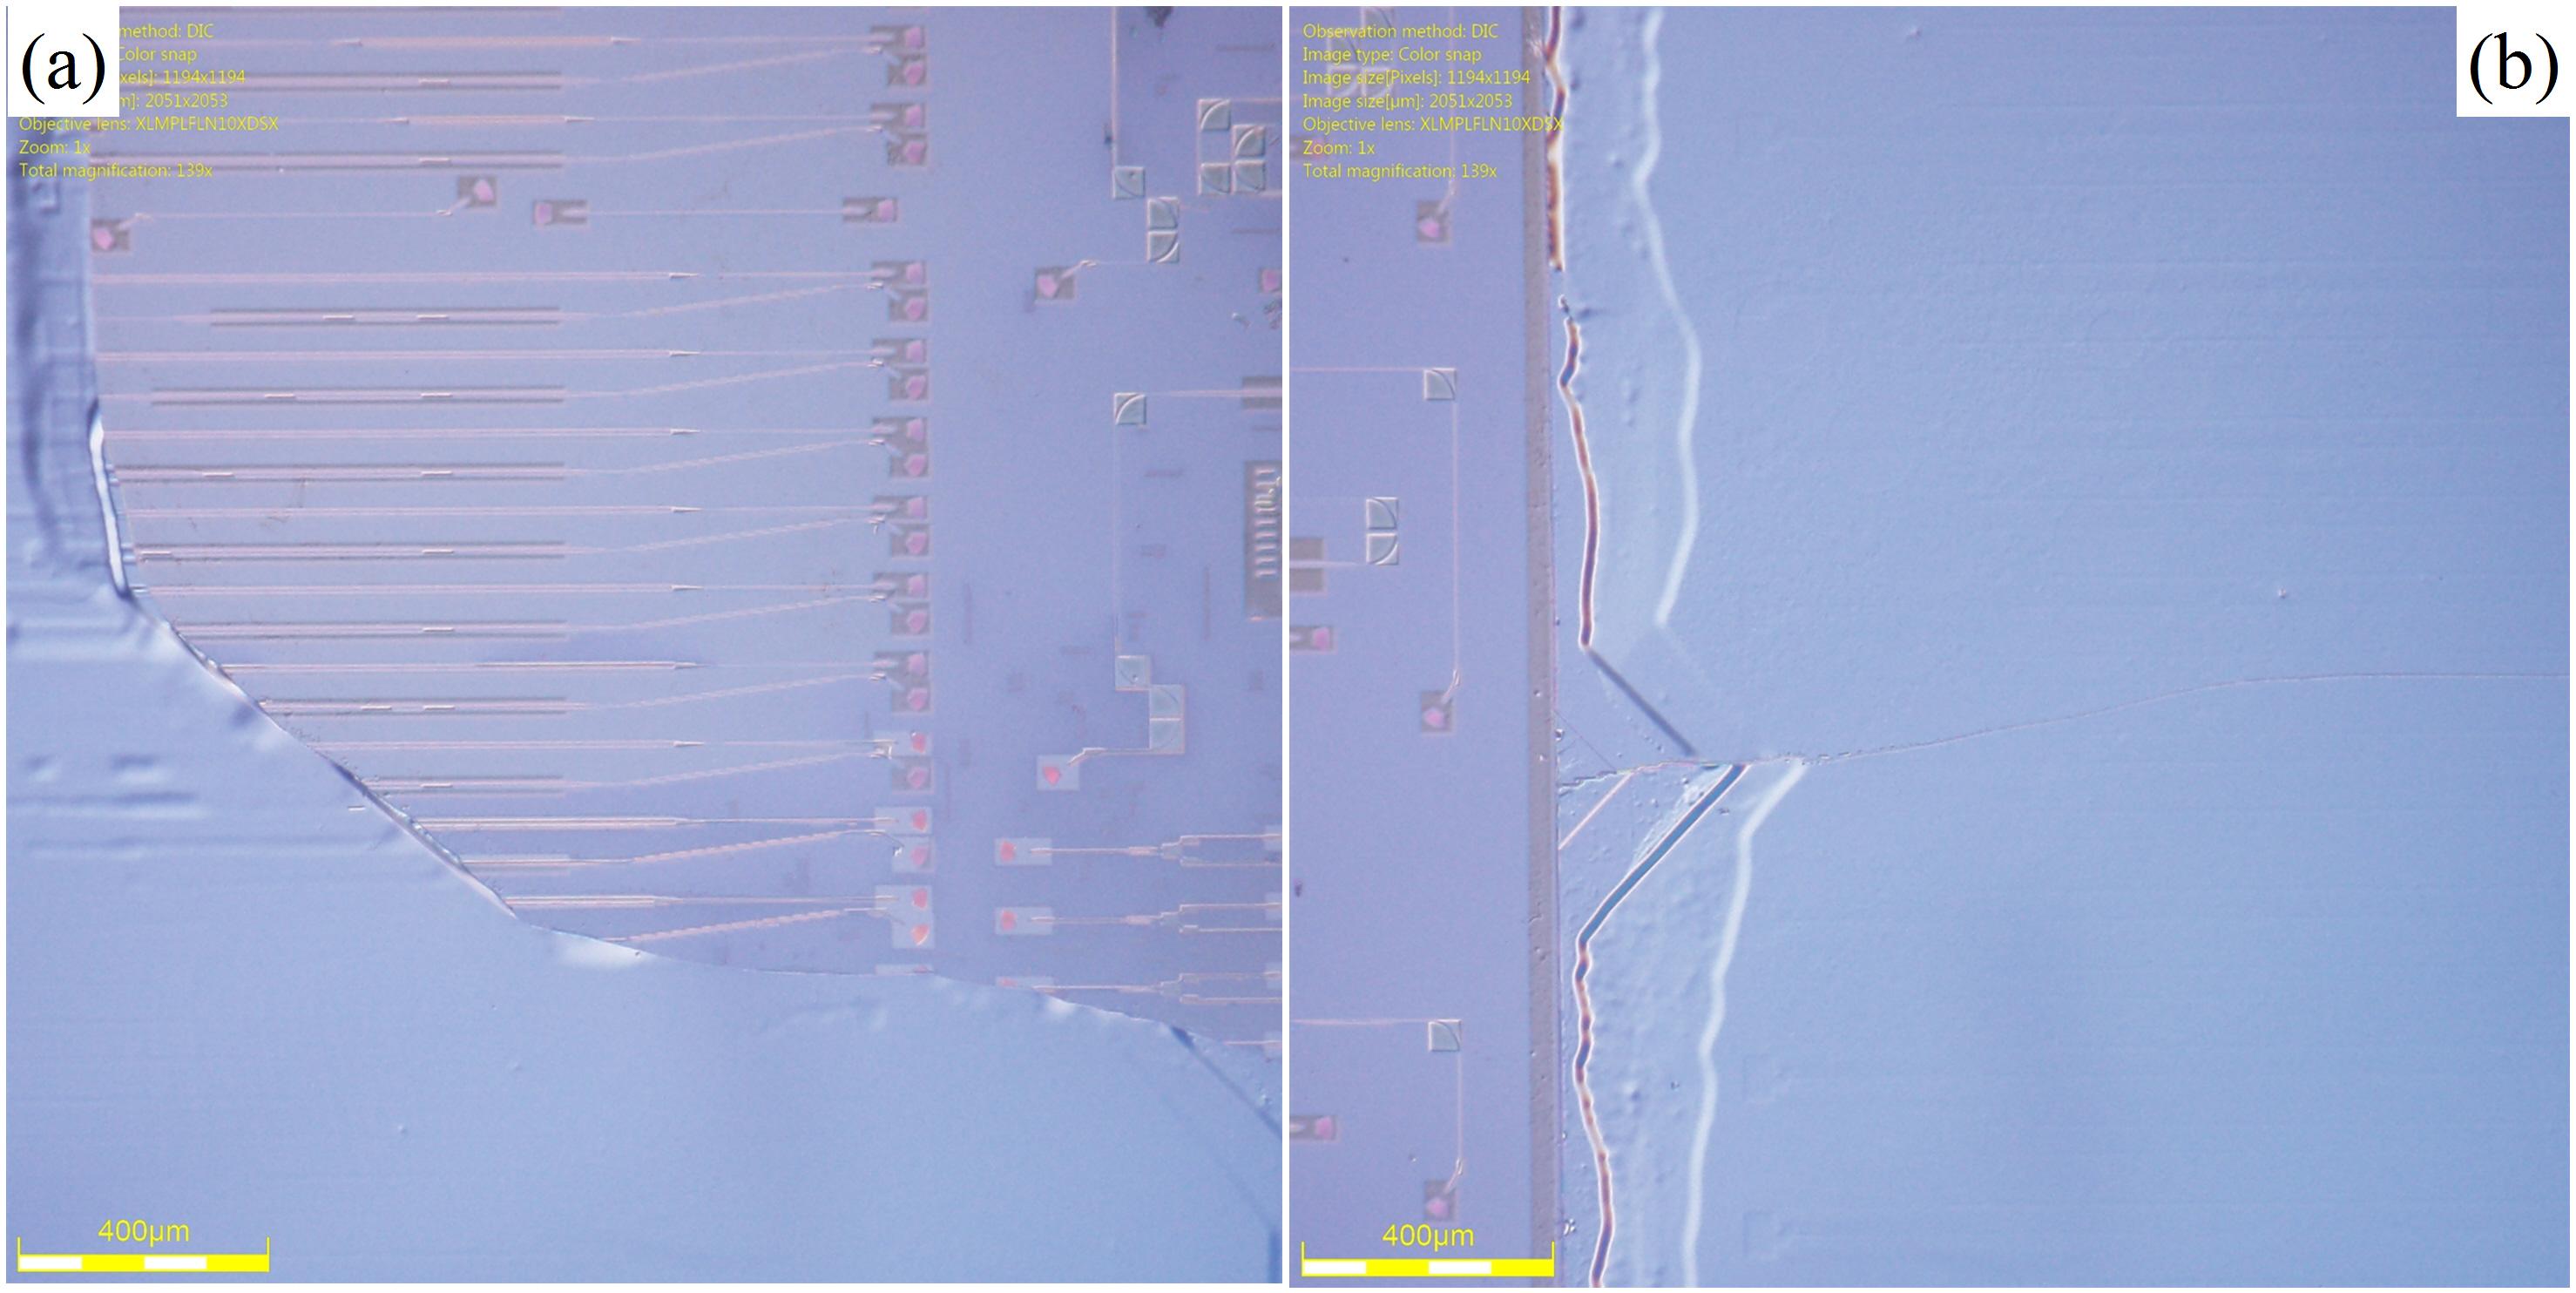
\includegraphics[width=14cm]{./Pictures/laser_sub_removal.jpg}
		\captionsetup{justification=centering}
		\caption{(a)因键合质量不好部分III-V芯片脱落;(b)去除衬底过程中的侧向腐蚀现象}
		\label{laser_sub_removal}
	\end{figure}
	\item 
	用食人鱼溶液H\SB{2}SO\SB{4}:H\SB{2}O\SB{2}:H\SB{2}O=1:1:18去除InGaAs牺牲层,用纯盐酸去除InP牺牲层,这里同第(2)步一样可以通过颜色变化来判断牺牲层是否去除干净。去除完牺牲层后芯片示意图如图\ref{laser_fab}(a)所示。
	
	\begin{figure}[htb]
		\centering
		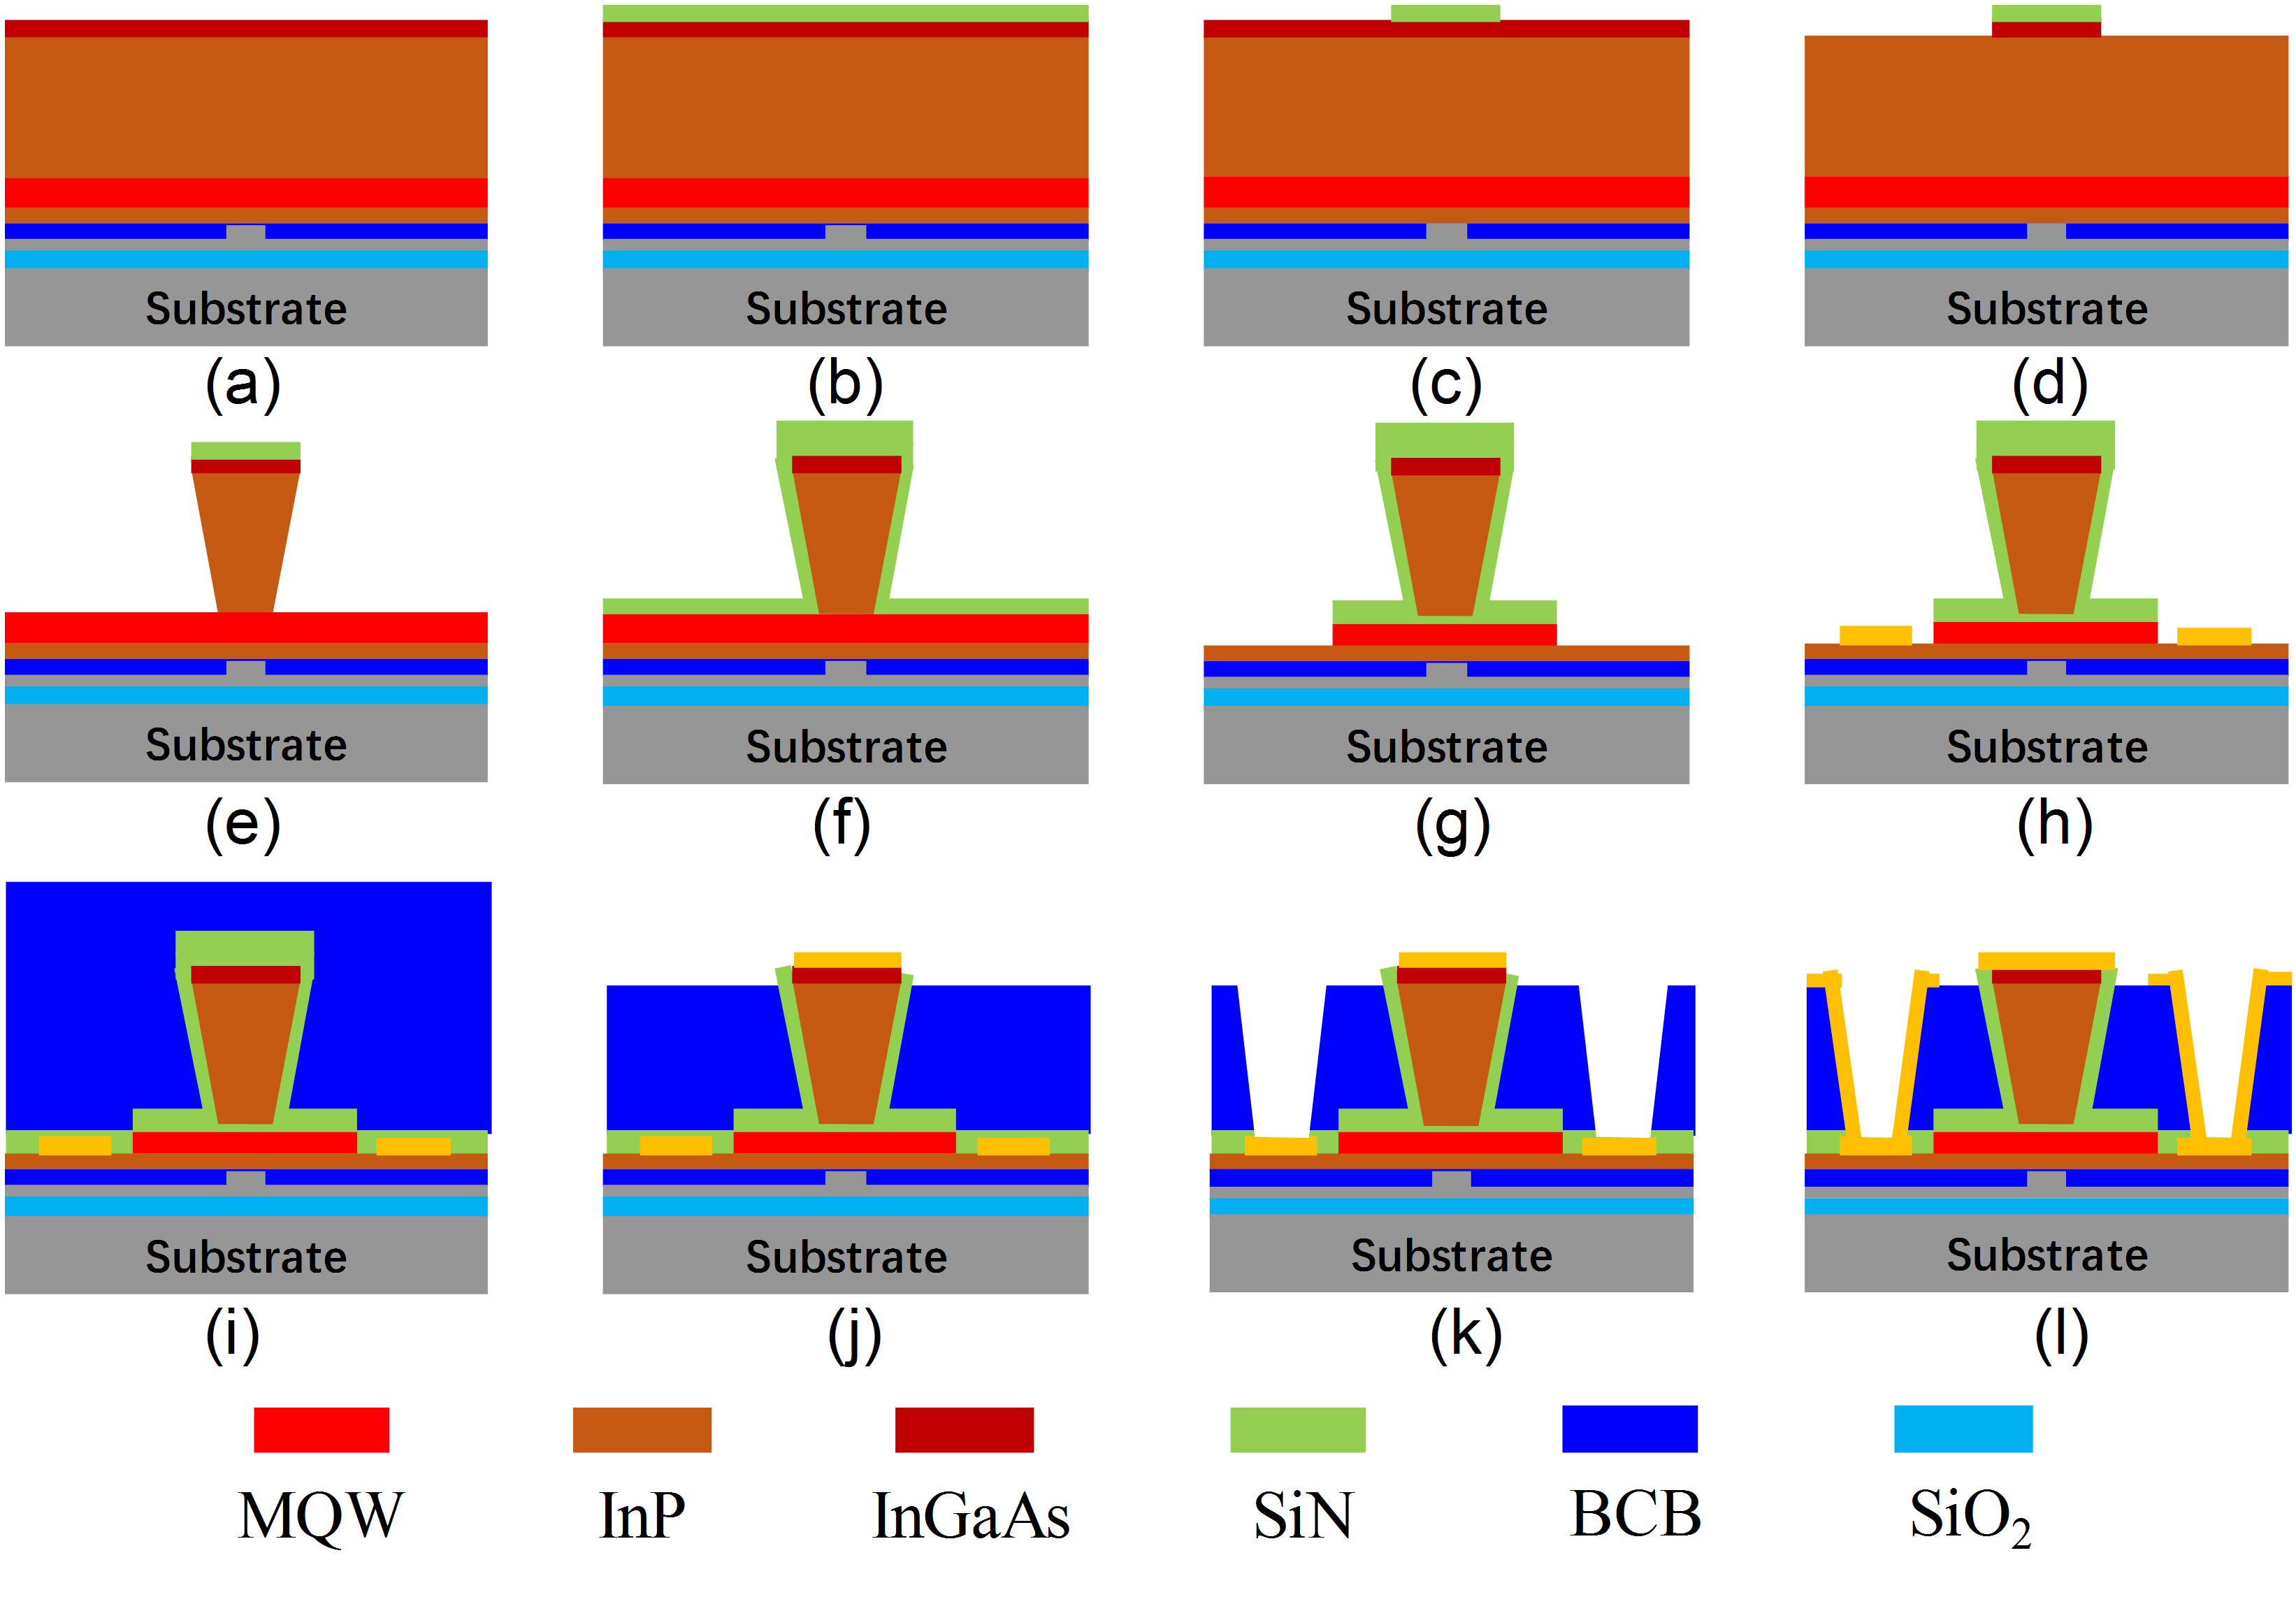
\includegraphics[width=15cm]{./Pictures/laser_fab.jpg}
		\captionsetup{justification=centering}
		\caption{硅基III-V混合集成自脉冲DFB激光器工艺流程示意图,(a)\~{}(l)展示了不同步骤下的波导截面图}
		\label{laser_fab}
	\end{figure}

	\item 
	从这一步开始开始制作III-V波导,首先在p-InGaAs上沉积5~$nm$~SiO\SB{2}和200~$nm$~SiN作为掩模,芯片示意图如图\ref{laser_fab}(b)所示。
	\item 
	利用SOI芯片上的套刻标记,光刻制作p-InGaAs层的结构。先将芯片放于120 $^{\circ}$C的热板上去水汽5~$min$以上,然后将芯片放置于常温金属块上冷却之后,旋涂增粘剂Ti Prime,4000 rpm 40~$s$,之后120 $^{\circ}$C烘烤3 $min$,以增强芯片与光刻胶的粘附性。因为该层图案宽度较小,最窄处只有750~$nm$,如果粘附性不好,光刻胶就很容易掉落。烘烤之后旋涂高分辨率光刻胶MIR 701,4000~rpm 40~$s$,之后100~$^{\circ}$C烘烤1~$min$~20~$s$。接下去进行接触式曝光,曝光时间为120 $s$,光刻机采用S\.{U}SS MicroTec MA6,曝光波长为320~$nm$,功率为325~$W$,曝光时间为120~$s$。曝光完成需要后烘,110~$^{\circ}$C烘烤1~$min$。之后用MIF显影液显影,通过芯片表面的彩色条纹全部退去判断显影是否完成,用显微镜检查曝光质量,如果p-InGaAs层颜色均匀,说明曝光质量可以接受。最后用反应离子刻蚀机(Reactive Ion Etching, RIE)刻蚀SiN,刻蚀时间为2~$min$~30~$s$。刻蚀完成后用丙酮,异丙醇,水清洗刻蚀完之后的芯片,去除残留的光刻胶,此时的芯片示意图如图\ref{laser_fab}(c)所示。
	\item 
	用ICP刻蚀InGaAs,刻蚀气体为CH\SB{4}和H\SB{2},采用多个周期刻蚀,每个周期刻蚀深度约为50~$nm$。通过台阶仪判断刻蚀终点,刻蚀深度要大于220 $nm$以保证InGaAs已经刻蚀完,否则会造成下一步湿法腐蚀无法进行,此时芯片示意图如图\ref{laser_fab}(d)所示。
	\item
	用HCl:H\SB{2}O=1:1溶液湿法腐蚀InP,这一步中可以使用摇床加快腐蚀速度。由于InP的腐蚀有晶向特性,故最终会形成倒梯形结构,使得模式能够更好的限制在多量子阱层,降低激光器的阈值电流。如果在键合的时候III-V芯片的晶向放置错误,这一步就会形成正梯形的结构,模式在有源区中的限制因子就会降低,使得激光器的阈值电流增大。该步通过分步多次腐蚀划台阶仪的方法来确定腐蚀终点,越接近终点,腐蚀间隔取的越短,当两次腐蚀深度不再增加的时候,即可判断已经腐蚀到多量子阱层。此步完成之后的芯片示意图如图\ref{laser_fab}(e)所示。
	\item 
	用PECVD沉积200~$nm$左右的SiN保护InP侧壁和作为制作多量子阱层的掩模,此时芯片示意图如图\ref{laser_fab}(f)所示。
	\item 
	光刻制作多量子阱层的结构。该步依然采用Ti Prime与MIR 701,此时将MIR 701的转速降为3000 rpm,其他参数与(9)相同,用RIE刻蚀SiN,ICP刻蚀多量子阱层。我们采用宽度为9~$\mu m$的量子阱宽度,这样可以减小ICP刻蚀造成的表面缺陷态对载流子的影响。此时芯片示意图如图\ref{laser_fab}(g)所示。
	\item 
	光刻制作n金属接触(n-contact)结构。此步采用光刻胶Ti 35E,匀胶参数为3000 rpm 40 $s$,100 $^{\circ}$C烘烤3 $min$,曝光时间为55 $s$,等10分钟后,再125 $^{\circ}$C烘烤2 $min$,之后空曝185~$s$做图像反转,用AZ400:H\SB{2}O = 1:3显影1 $min$ 20 $s$。然后用RIE刻蚀几秒钟去除可能残留的光刻胶,再在H\SB{2}SO\SB{4}:H\SB{2}O\SB{2}:H\SB{2}O=1:1:20溶液中快速浸5 $s$去除可能存在的氧化层,此步需要在蒸镀之前尽量短的时间内做以避免再次被氧化。最后蒸镀金属Ni:Ge:Au= 30~$nm$:20~$nm$:50~$nm$,利用剥离工艺(lift-off)去除多余金属。此时芯片示意图如图\ref{laser_fab}(h)所示。
	\item 
	光刻制作n-InP层上的结构。先旋涂Ti Prime,参数与(9)中相同,然后旋涂光刻胶AZ 9260,3000~rpm 40~$s$,之后100 $^{\circ}$C烘烤40~$s$,曝光200~$s$。曝光之后用AZ400:H\SB{2}O = 1:2显影2~$min$~30~$s$。用HCl:H\SB{2}O = 1:1溶液将没有被光刻胶保护的n-InP腐蚀掉,此步可以通过颜色和台阶仪共同确定腐蚀终点,如图\ref{laser_island}所示。再用丙酮,异丙醇去掉光刻胶,沉积600~$nm$~SiN做钝化处理。
	\begin{figure}[htb]
		\centering
		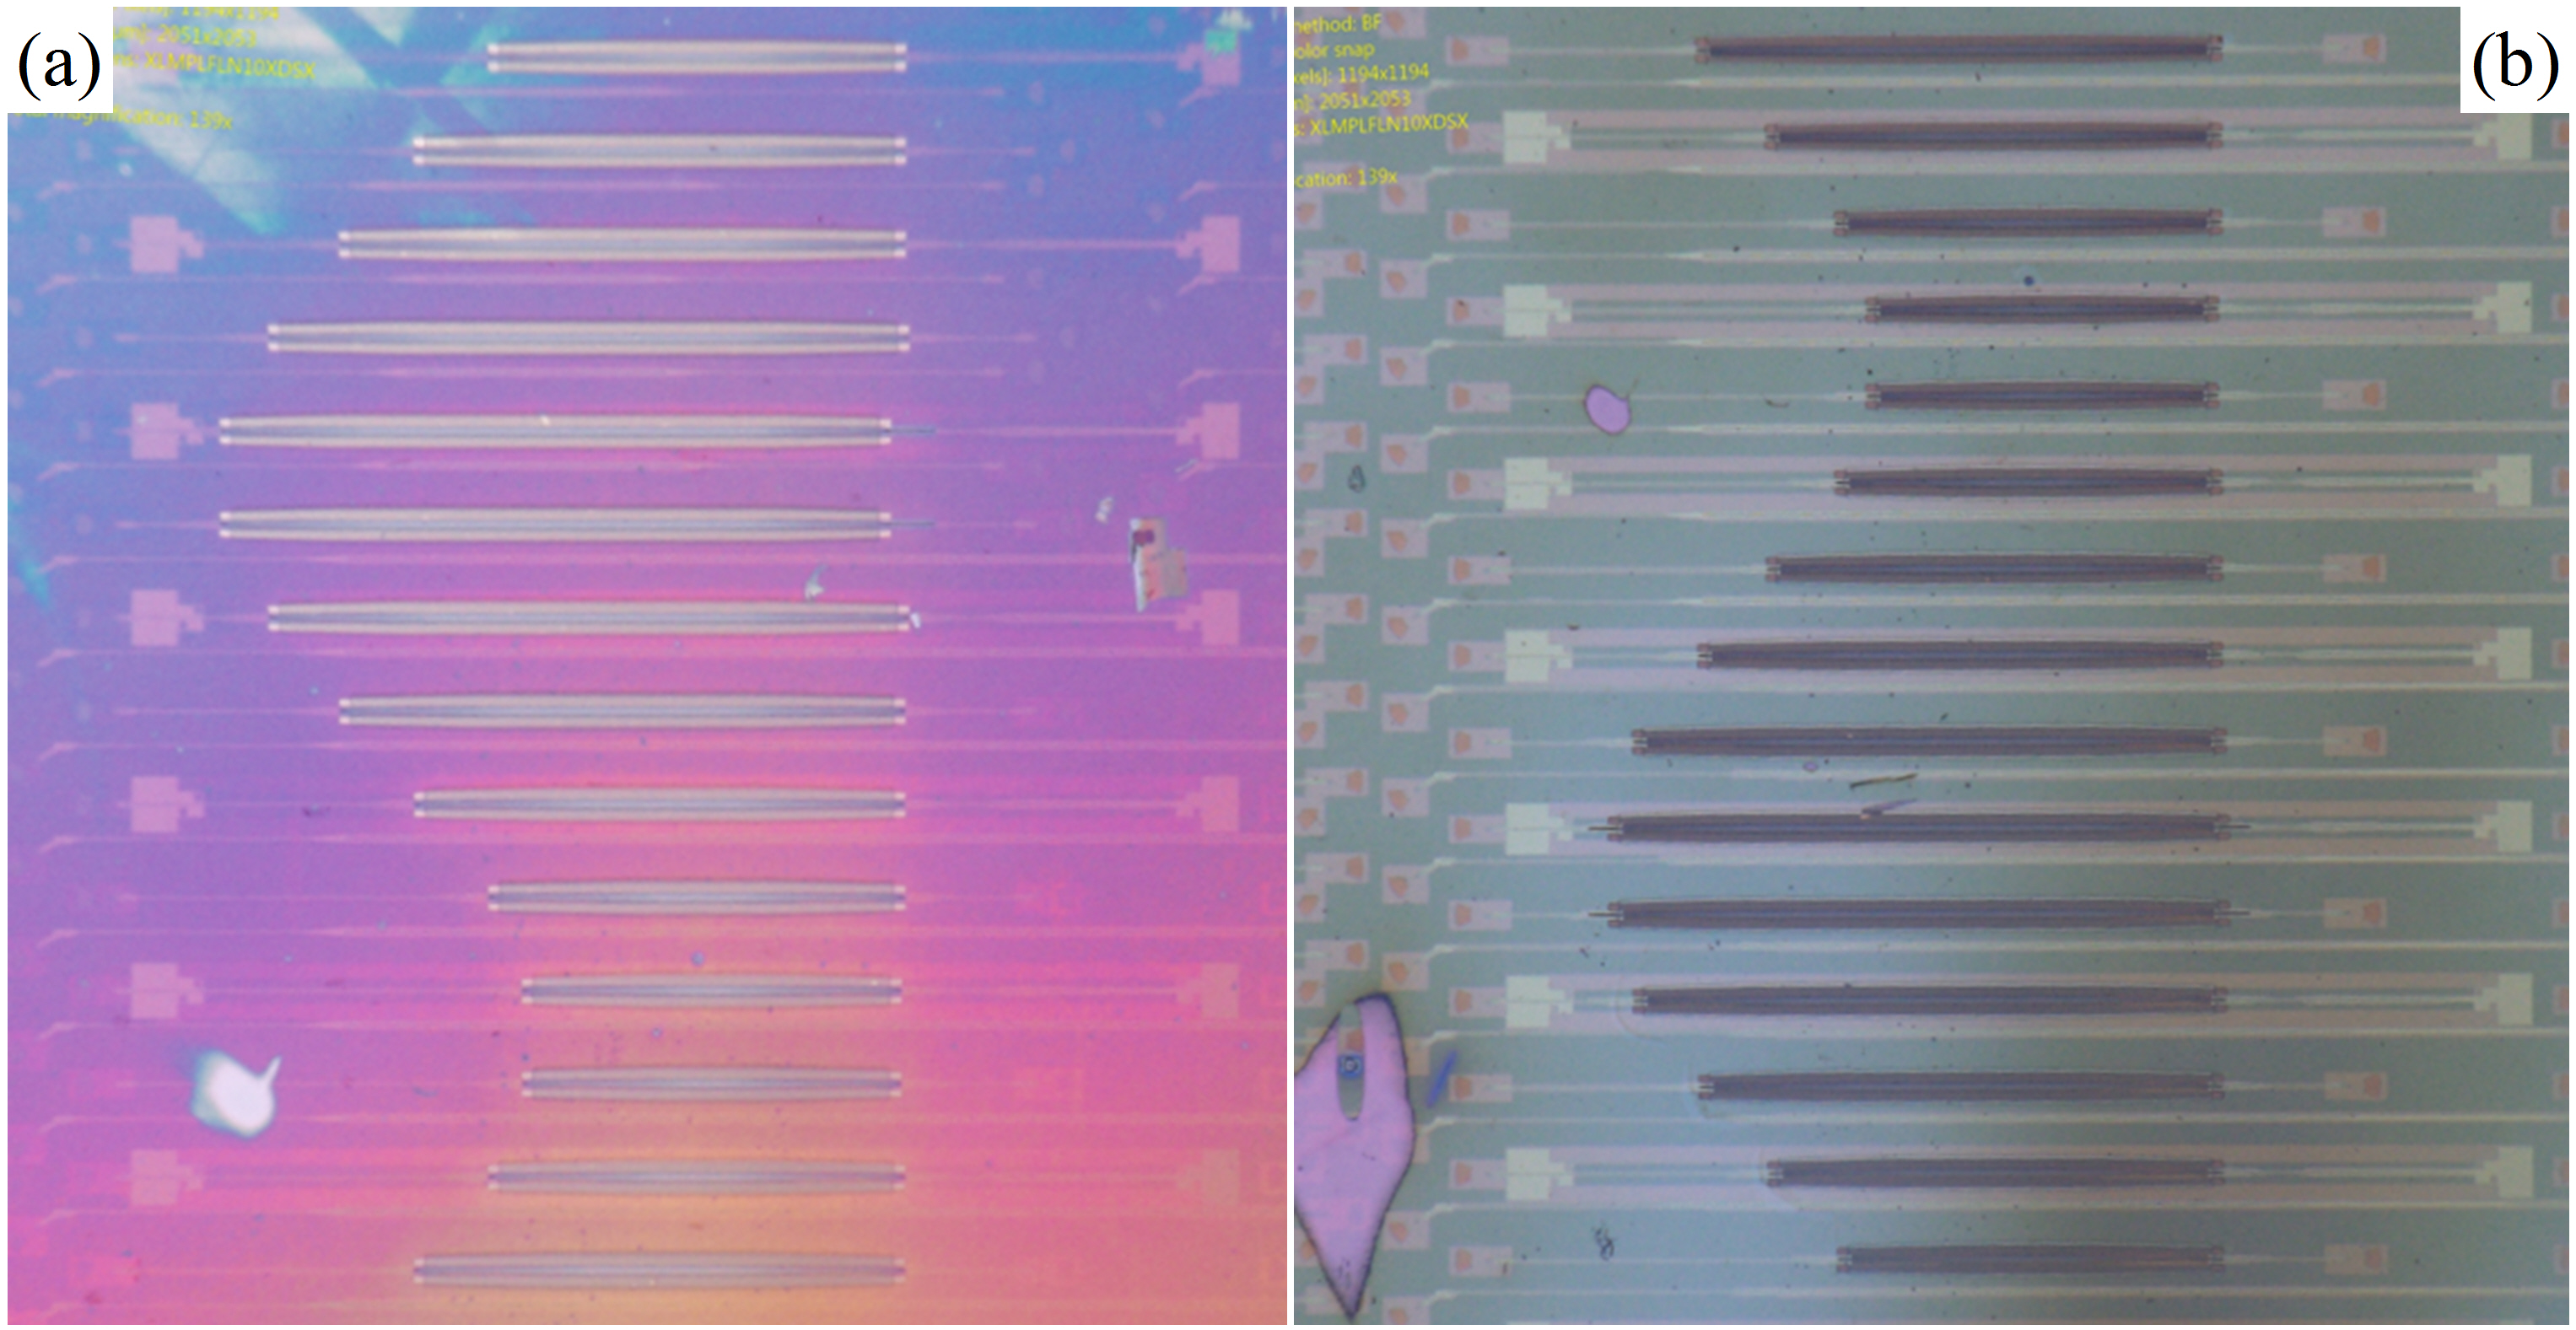
\includegraphics[width=14cm]{./Pictures/laser_island.jpg}
		\captionsetup{justification=centering}
		\caption{(a)~n-InP还未腐蚀干净;(b)~n-InP已经腐蚀干净}
		\label{laser_island}
	\end{figure}
	\item 
	旋涂BCB 3022-57做平坦化处理,转速2000 rpm 40~$s$,以得到较厚的BCB,超过III-V波导的高度。然后用烘箱280 $^{\circ}$C烘烤2小时使其玻璃化,之后用来承载电极。此时芯片示意图如图\ref{laser_fab}(i)所示。
	\item 
	使用RIE回刻BCB至InGaAs上的SiN处,通过台阶仪判断刻蚀终点。然后RIE换配方刻蚀完InGaAs上的SiN,光刻制作InGaAs中间的刻蚀部分,用光刻胶Ti 35E,参数与(14)中相同,然后ICP刻蚀InGaAs,刻蚀深度需要保证大于220~$nm$,使得两段电极分离。
	\begin{figure}[htb]
		\centering
		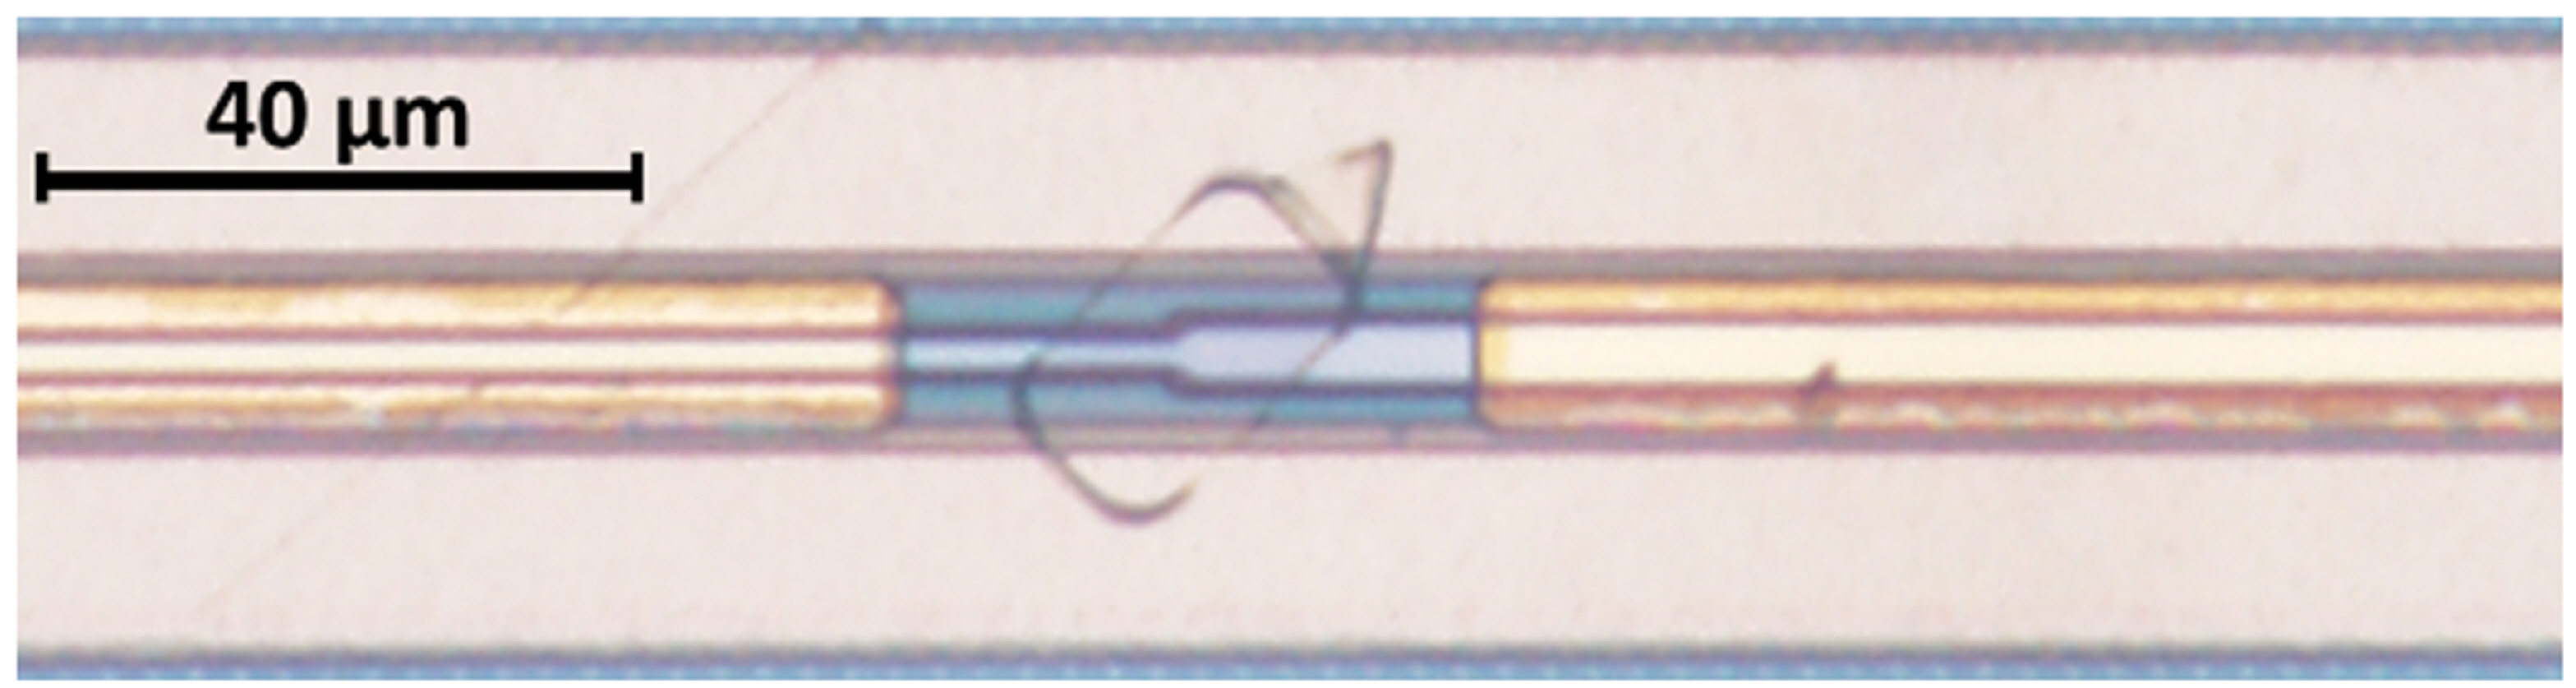
\includegraphics[width=14cm]{./Pictures/laser_cut.jpg}
		\captionsetup{justification=centering}
		\caption{p-contact中间的电隔离区域}
		\label{laser_cut}
	\end{figure}
	\item 
	光刻制作p金属接触结构(p-contact)的结构,采用Ti Prime和光刻胶Ti 35E,参数与(14)中相同,曝光之后反转。显影之后,蒸镀前利用RIE刻蚀30~$s$去掉残留的光刻胶,用H\SB{2}SO\SB{4}:H\SB{2}O\SB{2}:H\SB{2}O=1:1:20溶液浸泡5~$s$去除氧化层。蒸镀Ti:Au=40~$nm$:150~$nm$,利用剥离工艺去除多余的金属。此时芯片示意图如图\ref{laser_fab}(j)所示,在显微镜下如图\ref{laser_cut}所示。
	\item
	使用RIE刻蚀BCB在n接触层上方开窗口,采用光刻胶Ti 35E光刻胶,参数与(14)中相同,用RIE刻蚀BCB和SiN,露出n接触层金属,此处可以用台阶仪来判断刻蚀终点,刻蚀完成芯片示意图如图\ref{laser_fab}(k)所示。
	\item 
	用氧气等离子体清洗电极表面,光刻最后的电极结构,采用光刻胶Ti 35E,参数与(14)中相同。利用RIE刻蚀30~$s$去掉残留的光刻胶,蒸镀Ti:Au=40~$nm$:800~$nm$,用剥离工艺去除多余的金属,完成器件的制作,芯片示意图如图\ref{laser_fab}(l)所示。
\end{enumerate}



最终制作完成的硅基混合集成自脉冲DFB激光器如图\ref{laser_fabricationresult}(a)所示。使用FIB观察激光器的截面图如图\ref{laser_fabricationresult}(b)所示,几乎无法看到BCB键合层,说明BCB的厚度非常薄。从图中还可以看出光刻的套刻偏差在200~$nm$左右。

\begin{figure}[htb]
	\centering
	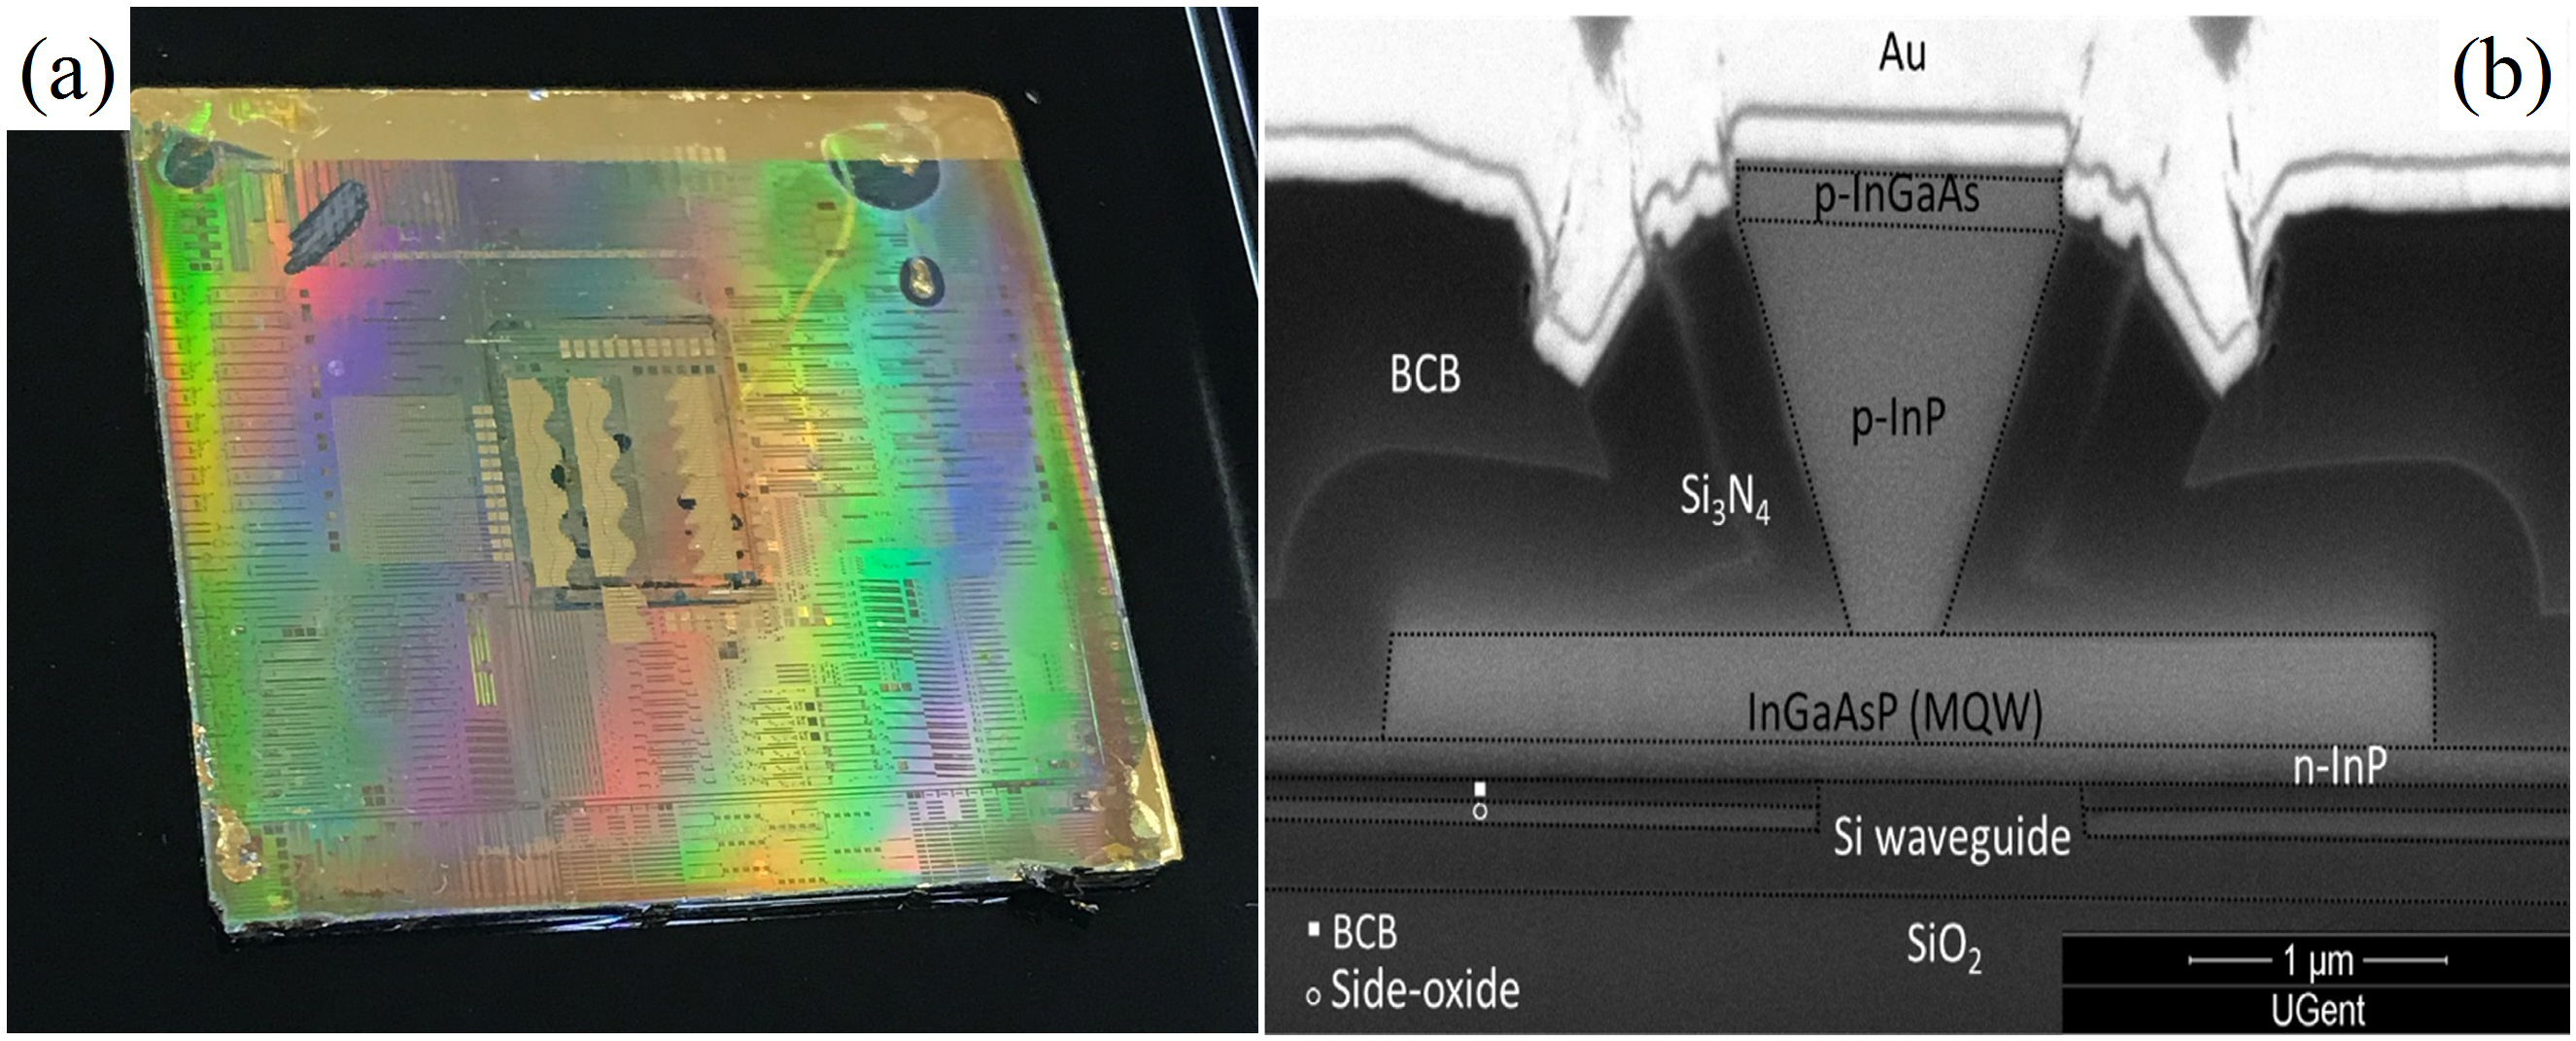
\includegraphics[width=15cm]{./Pictures/laser_fabricationresult.jpg}
	\captionsetup{justification=centering}
	\caption{(a)制作完成的硅基混合集成自脉冲DFB激光器芯片;(b)激光器截面SEM图,靠近III-V波导锥形结构尖端处}
	\label{laser_fabricationresult}
\end{figure}


\section{自脉冲激光器的静态性能测试}

\subsection{金属电极退火}

制作完激光器之后,首先需要进行I-V曲线测试,以判断器件是否能够正常工作。本文所制作该的自脉冲激光器,整体是个PIN结构,所以其I-V曲线也是标准的二极管响应曲线。当电极制作完成后,如果接触电阻过大,可以对器件进行快速退火处理,将金属电极与p接触层、n接触层的温度瞬间加热到极高的温度,改善它们之间的接触。常用的快速退火方法有脉冲激光退火与脉冲电子退火,本文为了方便采用的是电压快速退火法。通过在电极上加载一个比较高的电压,利用电阻产生的焦耳热直接对电极进行退火,可以对单个器件进行退火,而且本来对每个器件测试过程中就需要加载电压,故该方法适合实验中使用。该方法的缺点是如果电流太大,有可能将电极烧坏,故在退火时有需要限制最大电流的大小。

\begin{figure}[htb]
	\centering
	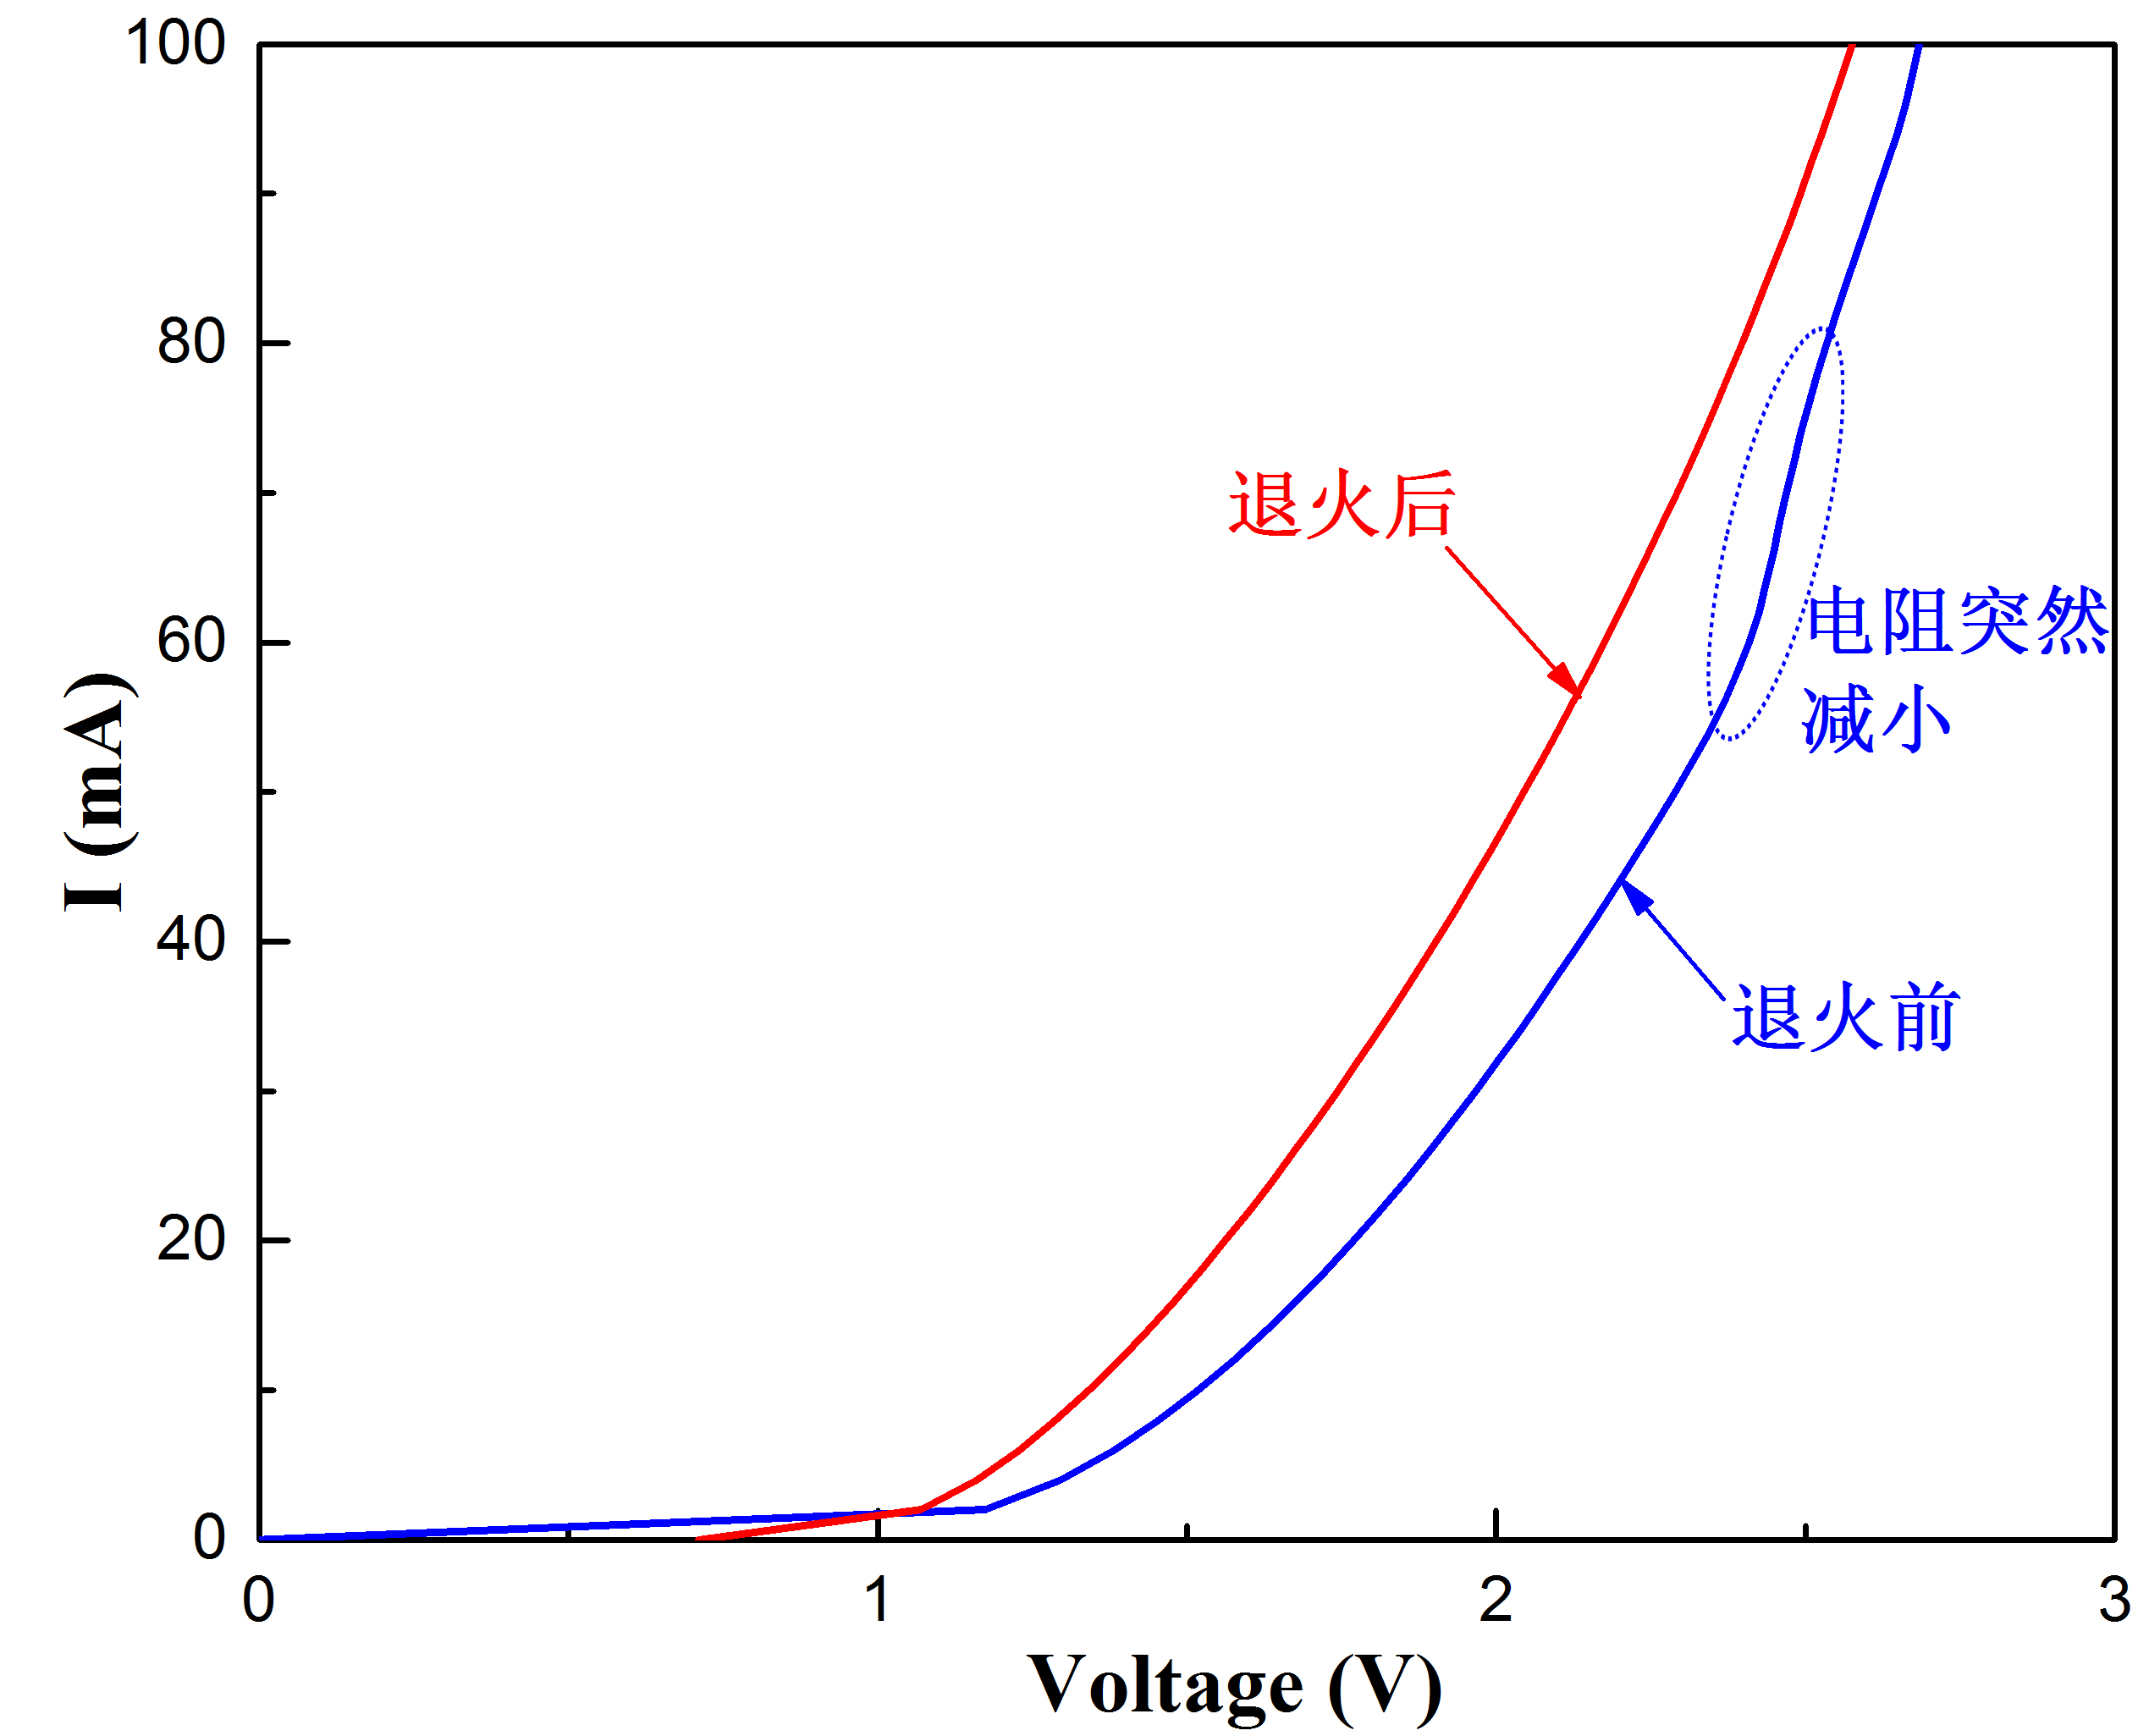
\includegraphics[width=12cm]{./Pictures/laser_annealing.jpg}
	\captionsetup{justification=centering}
	\caption{退火前与退火后自脉冲激光器的I-V曲线}
	\label{laser_annealing}
\end{figure}

图\ref{laser_annealing}中退火前的曲线是是将电流从0 $mA$逐渐增加到100 $mA$获得的,可以看到此时电压增加也比较快,但当电流增加到60 $mA$时,可以看到IV曲线中一个较明显的陡坡,对应着此时电阻瞬间较小,从而说明退火成功。当我们重新测试该器件的IV曲线时,可以发现退火后的IV曲线整体在退火前的IV曲线上方,说明退火之后的器件总电阻已经减小,该器件减小之后的总电阻在8.3 $\Omega$左右。 

\subsection{IV和PV曲线}

\begin{figure}[htb]
	\centering
	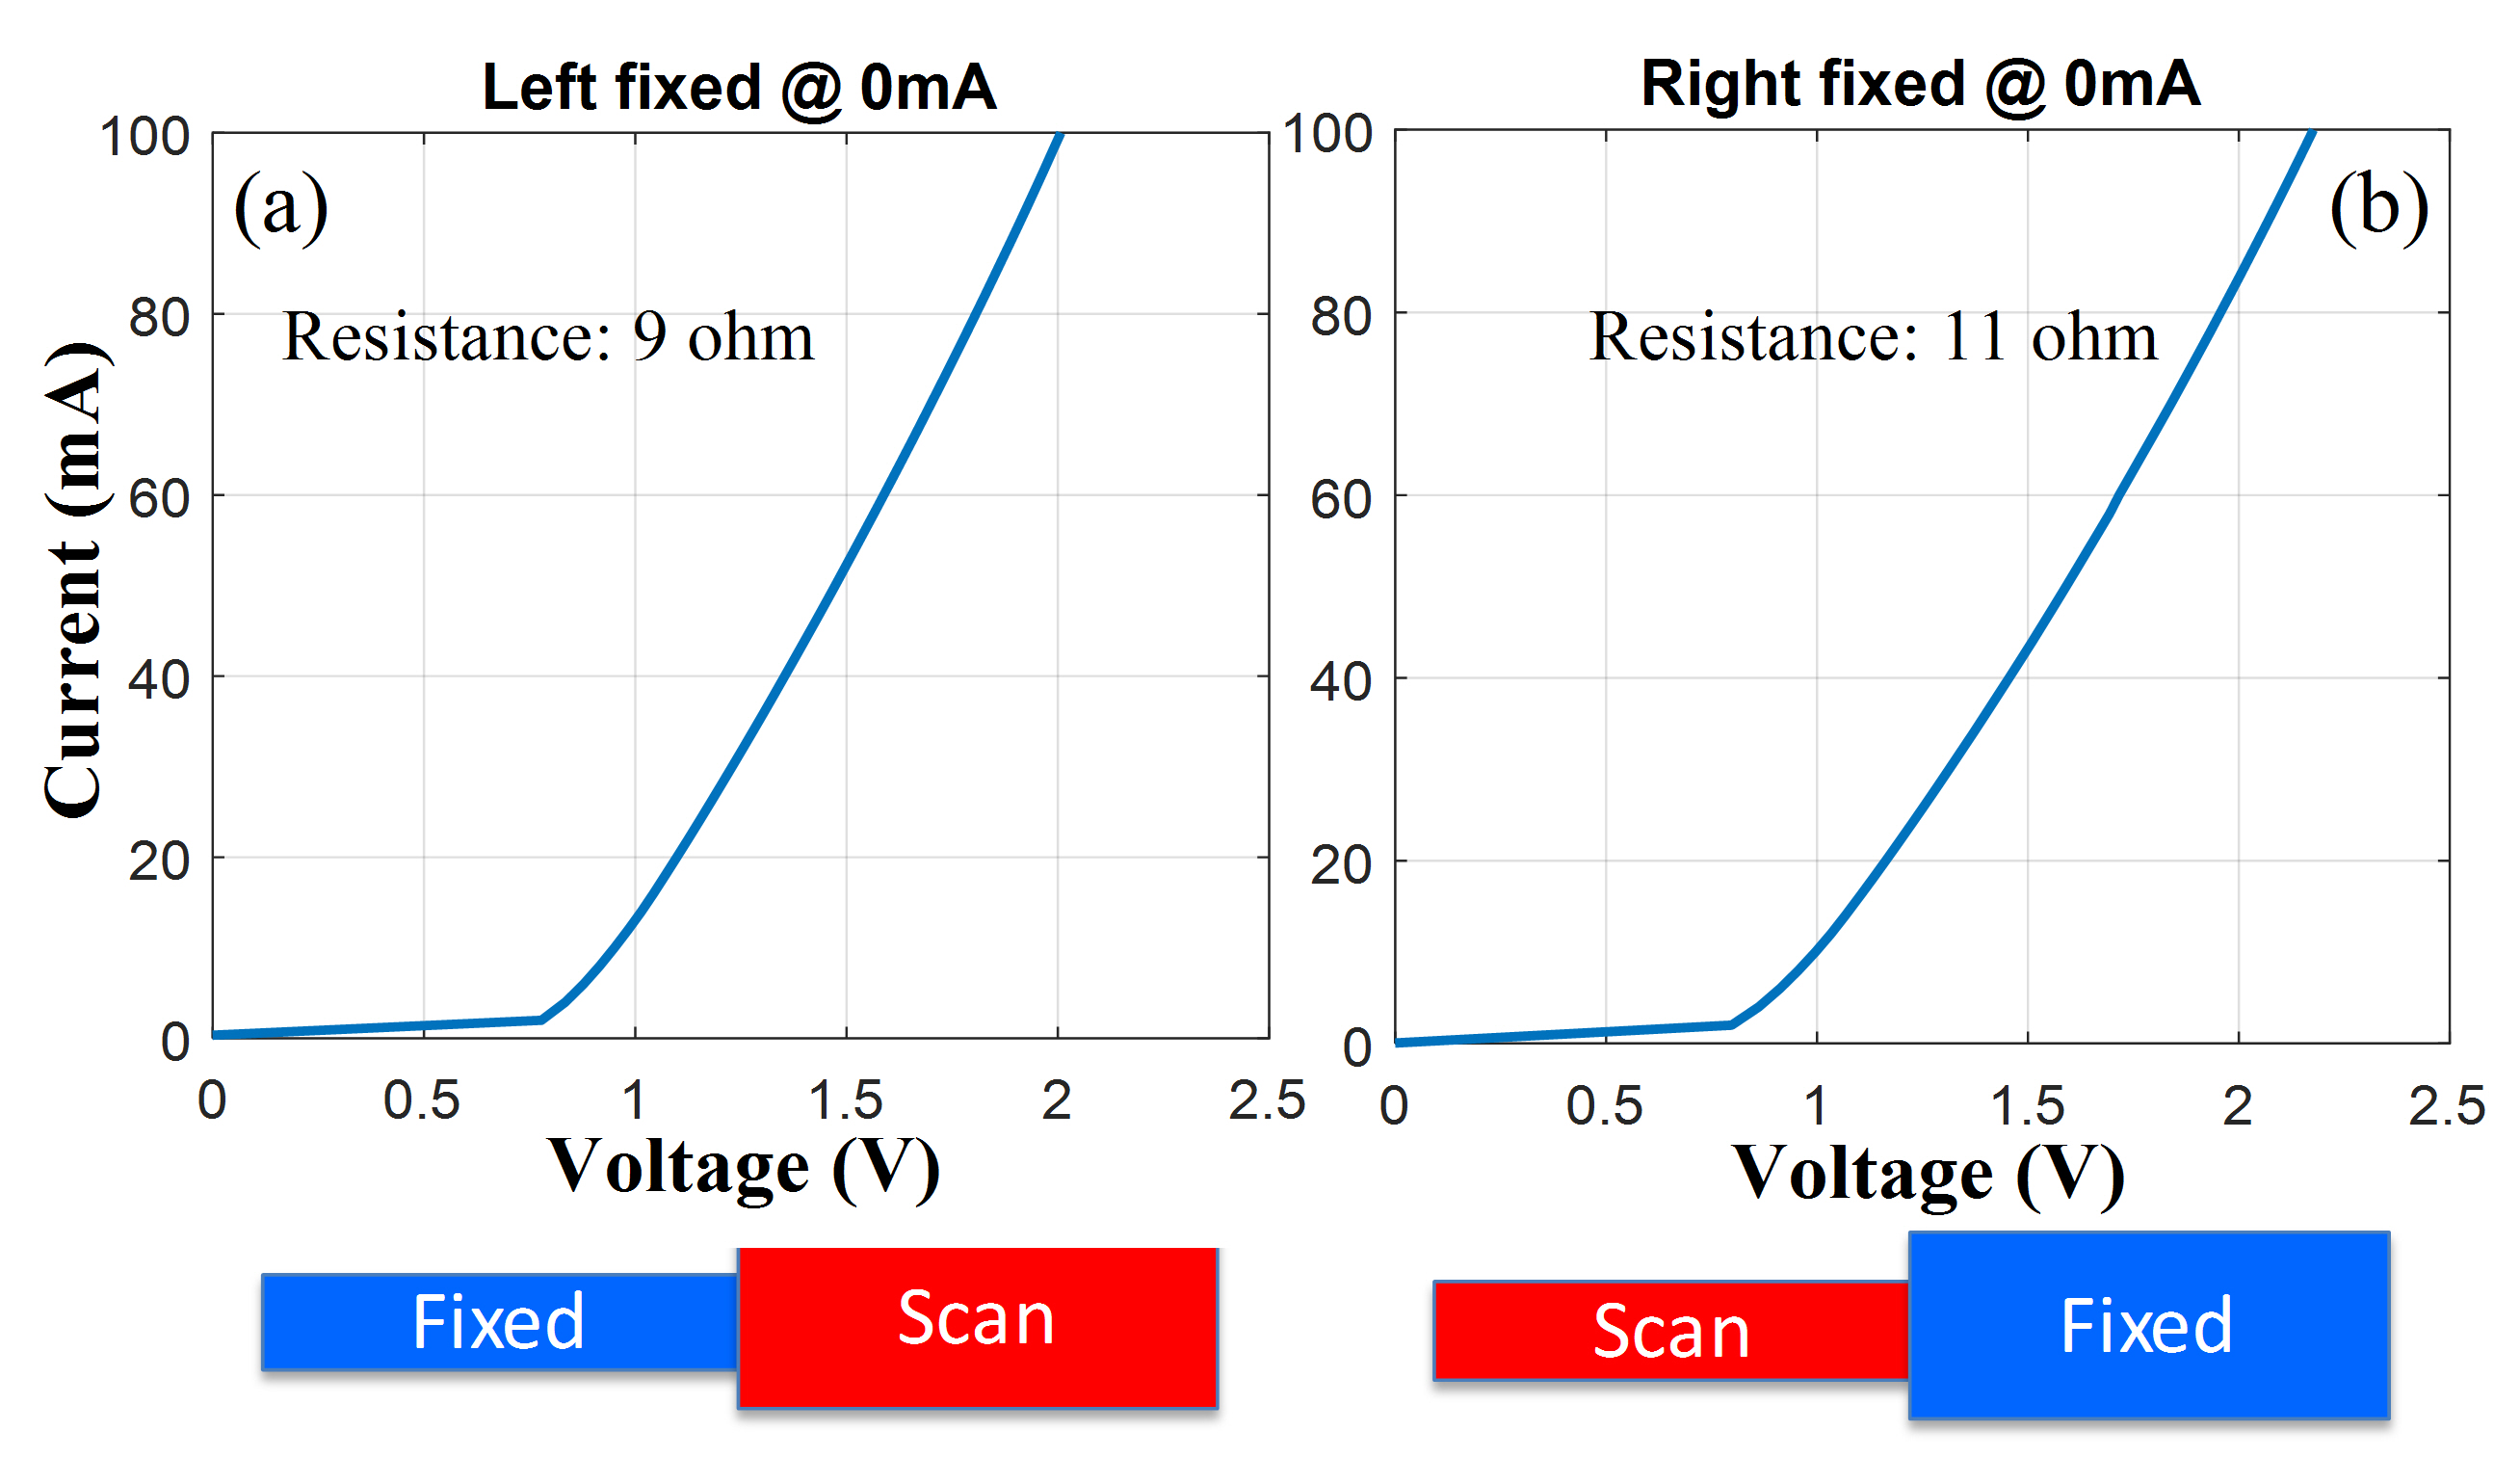
\includegraphics[width=15cm]{./Pictures/laser_IV.jpg}
	\captionsetup{justification=centering}
	\caption{两段式DFB激光器的IV响应曲线,(a)右段激光器的IV响应曲线;(b)左段激光器的IV响应曲线}
	\label{laser_IV}
\end{figure}

图\ref{laser_IV}给出了制作的某个激光器左右两段的IV响应曲线,测试温度为15$^{\circ}$C。该DFB激光器III-V波导由两段组成,总长度为900 $\mu m$。左边一段由长度为250~$\mu m$,宽度为2.5 $\mu m$的直波导和长度为230~$\mu m$的锥形波导构成,右边一段由长度为250~$\mu m$,宽度为4~$\mu m$的直波导和长度为230~$\mu m$的锥形波导构成。测试时,固定其中一段的电流为0~$mA$。从图中可以看出,左边一段的总电阻测得为11~$\Omega$,右边一段总电阻测得为9 $\Omega$,这与右边的电极与InGaAs接触面积较大相符合。

图\ref{laser_PI}给出了制作的某个激光器左右两段的的PI响应曲线,图中曲线的跳变处是由激光器的模式跳变引起。产生的激光通过左侧光栅耦合器耦合到光纤进行测试,从图中可以看到激光器输出到光纤的最大功率在-7~dBm左右,该PI响应曲线是在温度为15$^{\circ}$C时测得。我们分别测试了当其中一段激光器电流固定为0~$mA$、10~$mA$和50~$mA$时另一段激光器的PI响应曲线。当左段电流固定为I\SB{L} = 0~$mA$时,随着另一段电流的增加,输出功率逐渐增加,但最大功率在-20~dBm以下,这是由于此时左段激光器没有泵浦,激光从右段激光器产生,经过左段激光器时还会被部分吸收,故最大功率较低。当左段电流I\SB{L} = 10~$mA$时,输出功率最大值明显增大。当左段电流I\SB{L} = 50~$mA$时,输出功率一直处于较大的数值,而且随着右段电流的增加,输出功率还略微下降,这是由于当I\SB{L} = 50~$mA$时,左段激光器已处于激射状态且可以通过左侧的光栅直接输出,其在输出功率中占据了主要部分,即使在右段激光器没有激射时,输出功率也处于较高的水平,当右段电流增加时,反而使得整个激光器的温度上升,降低了左段激光器的发光效率,从而使得输出功率有所下降。当固定右段电流I\SB{R} = 0~$mA$或10~$mA$时,随着左段电流的增加,输出功率逐渐增加后饱和,此时PI响应曲线主要由左段激光器决定。当右段电流I\SB{R} = 50~$mA$时,可以看到当左段电流较小时,输出功率相对有所增加,增加部分由右段激光器提供。从图中还可以看到左右两段激光器的阈值电流都在12 $mA$左右。

\begin{figure}[htb]
	\centering
	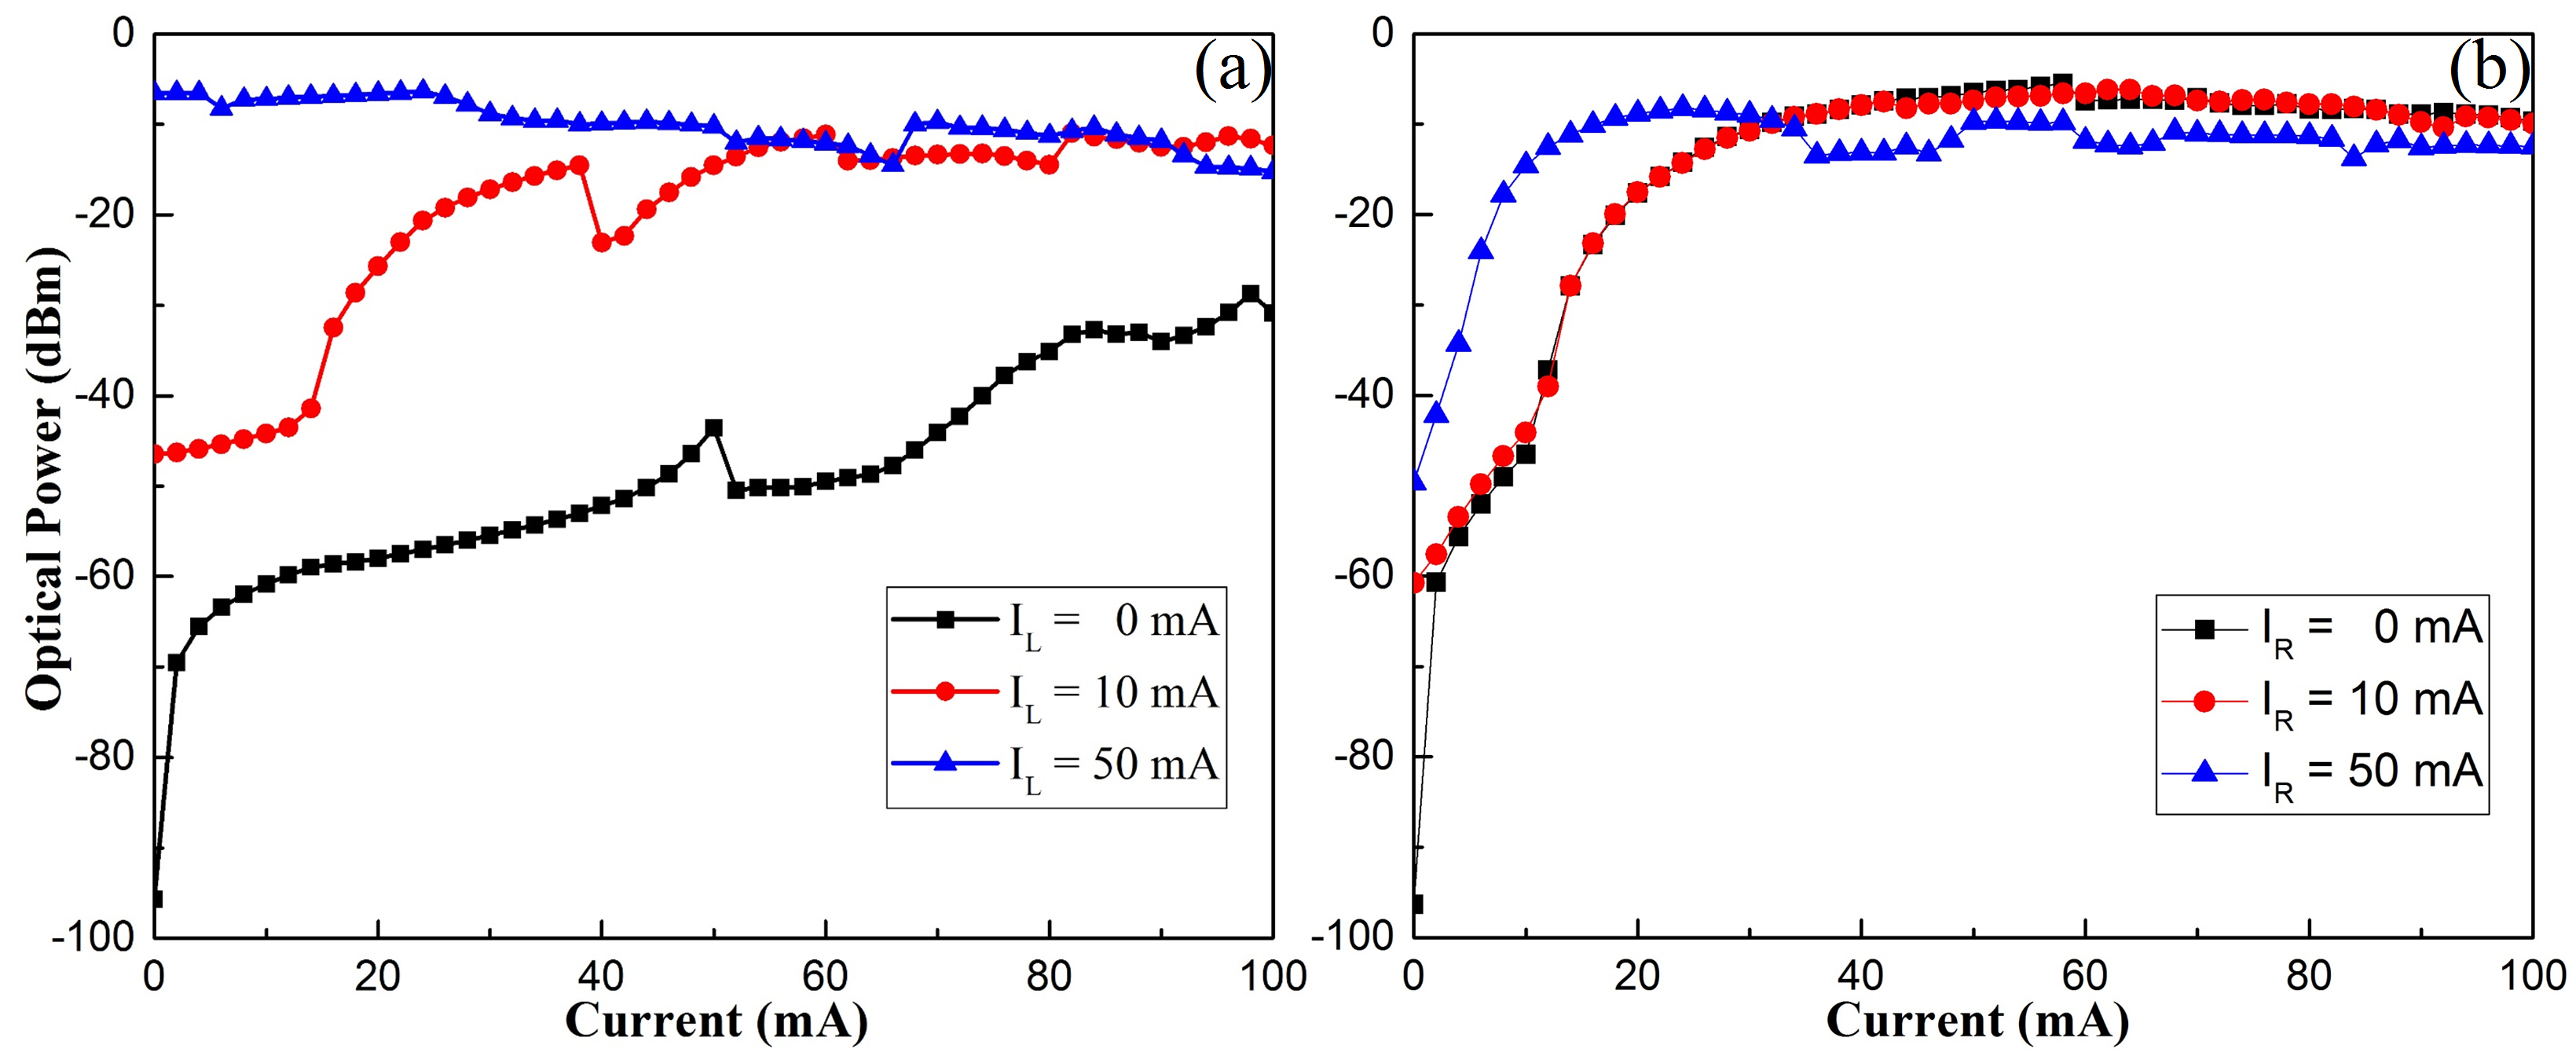
\includegraphics[width=15cm]{./Pictures/laser_PI.jpg}
	\captionsetup{justification=centering}
	\caption{两段式DFB激光器的PI响应曲线,激光从左边耦合光栅输出,(a)左段电流固定时,右段激光器PI响应曲线;(b)右段电流固定时,左段激光器PI响应曲线}
	\label{laser_PI}
\end{figure}

我们还测试了当观察到自脉冲信号时激光器的光谱如图\ref{laser_spectrum}所示:由于我们没有在每段激光器的DFB光栅中央提供$\lambda/4$的相移,故每段激光器会产生两个激射波长。当I\SB{L} = 32 $mA$,I\SB{R} = 35 $mA$时,其中间两个激射波长差为0.31~$nm$,将其输入一个高速探测器(photon detector, PD),通过电频谱仪观察到了38.75 GHz的自脉冲信号;当I\SB{L} = 32 $mA$,I\SB{R} = 50 $mA$时,其中间两个激射波长差为0.89~$nm$,对应的频率为110 GHz,超过了探测器的响应范围,故无法看到对应的自脉冲信号。从光谱中还可以看出该激光器布拉格反射镜的阻带宽度为4.2 $nm$左右,对应的耦合系数约为150 $cm^{-3}$。

\begin{figure}[htb]
	\centering
	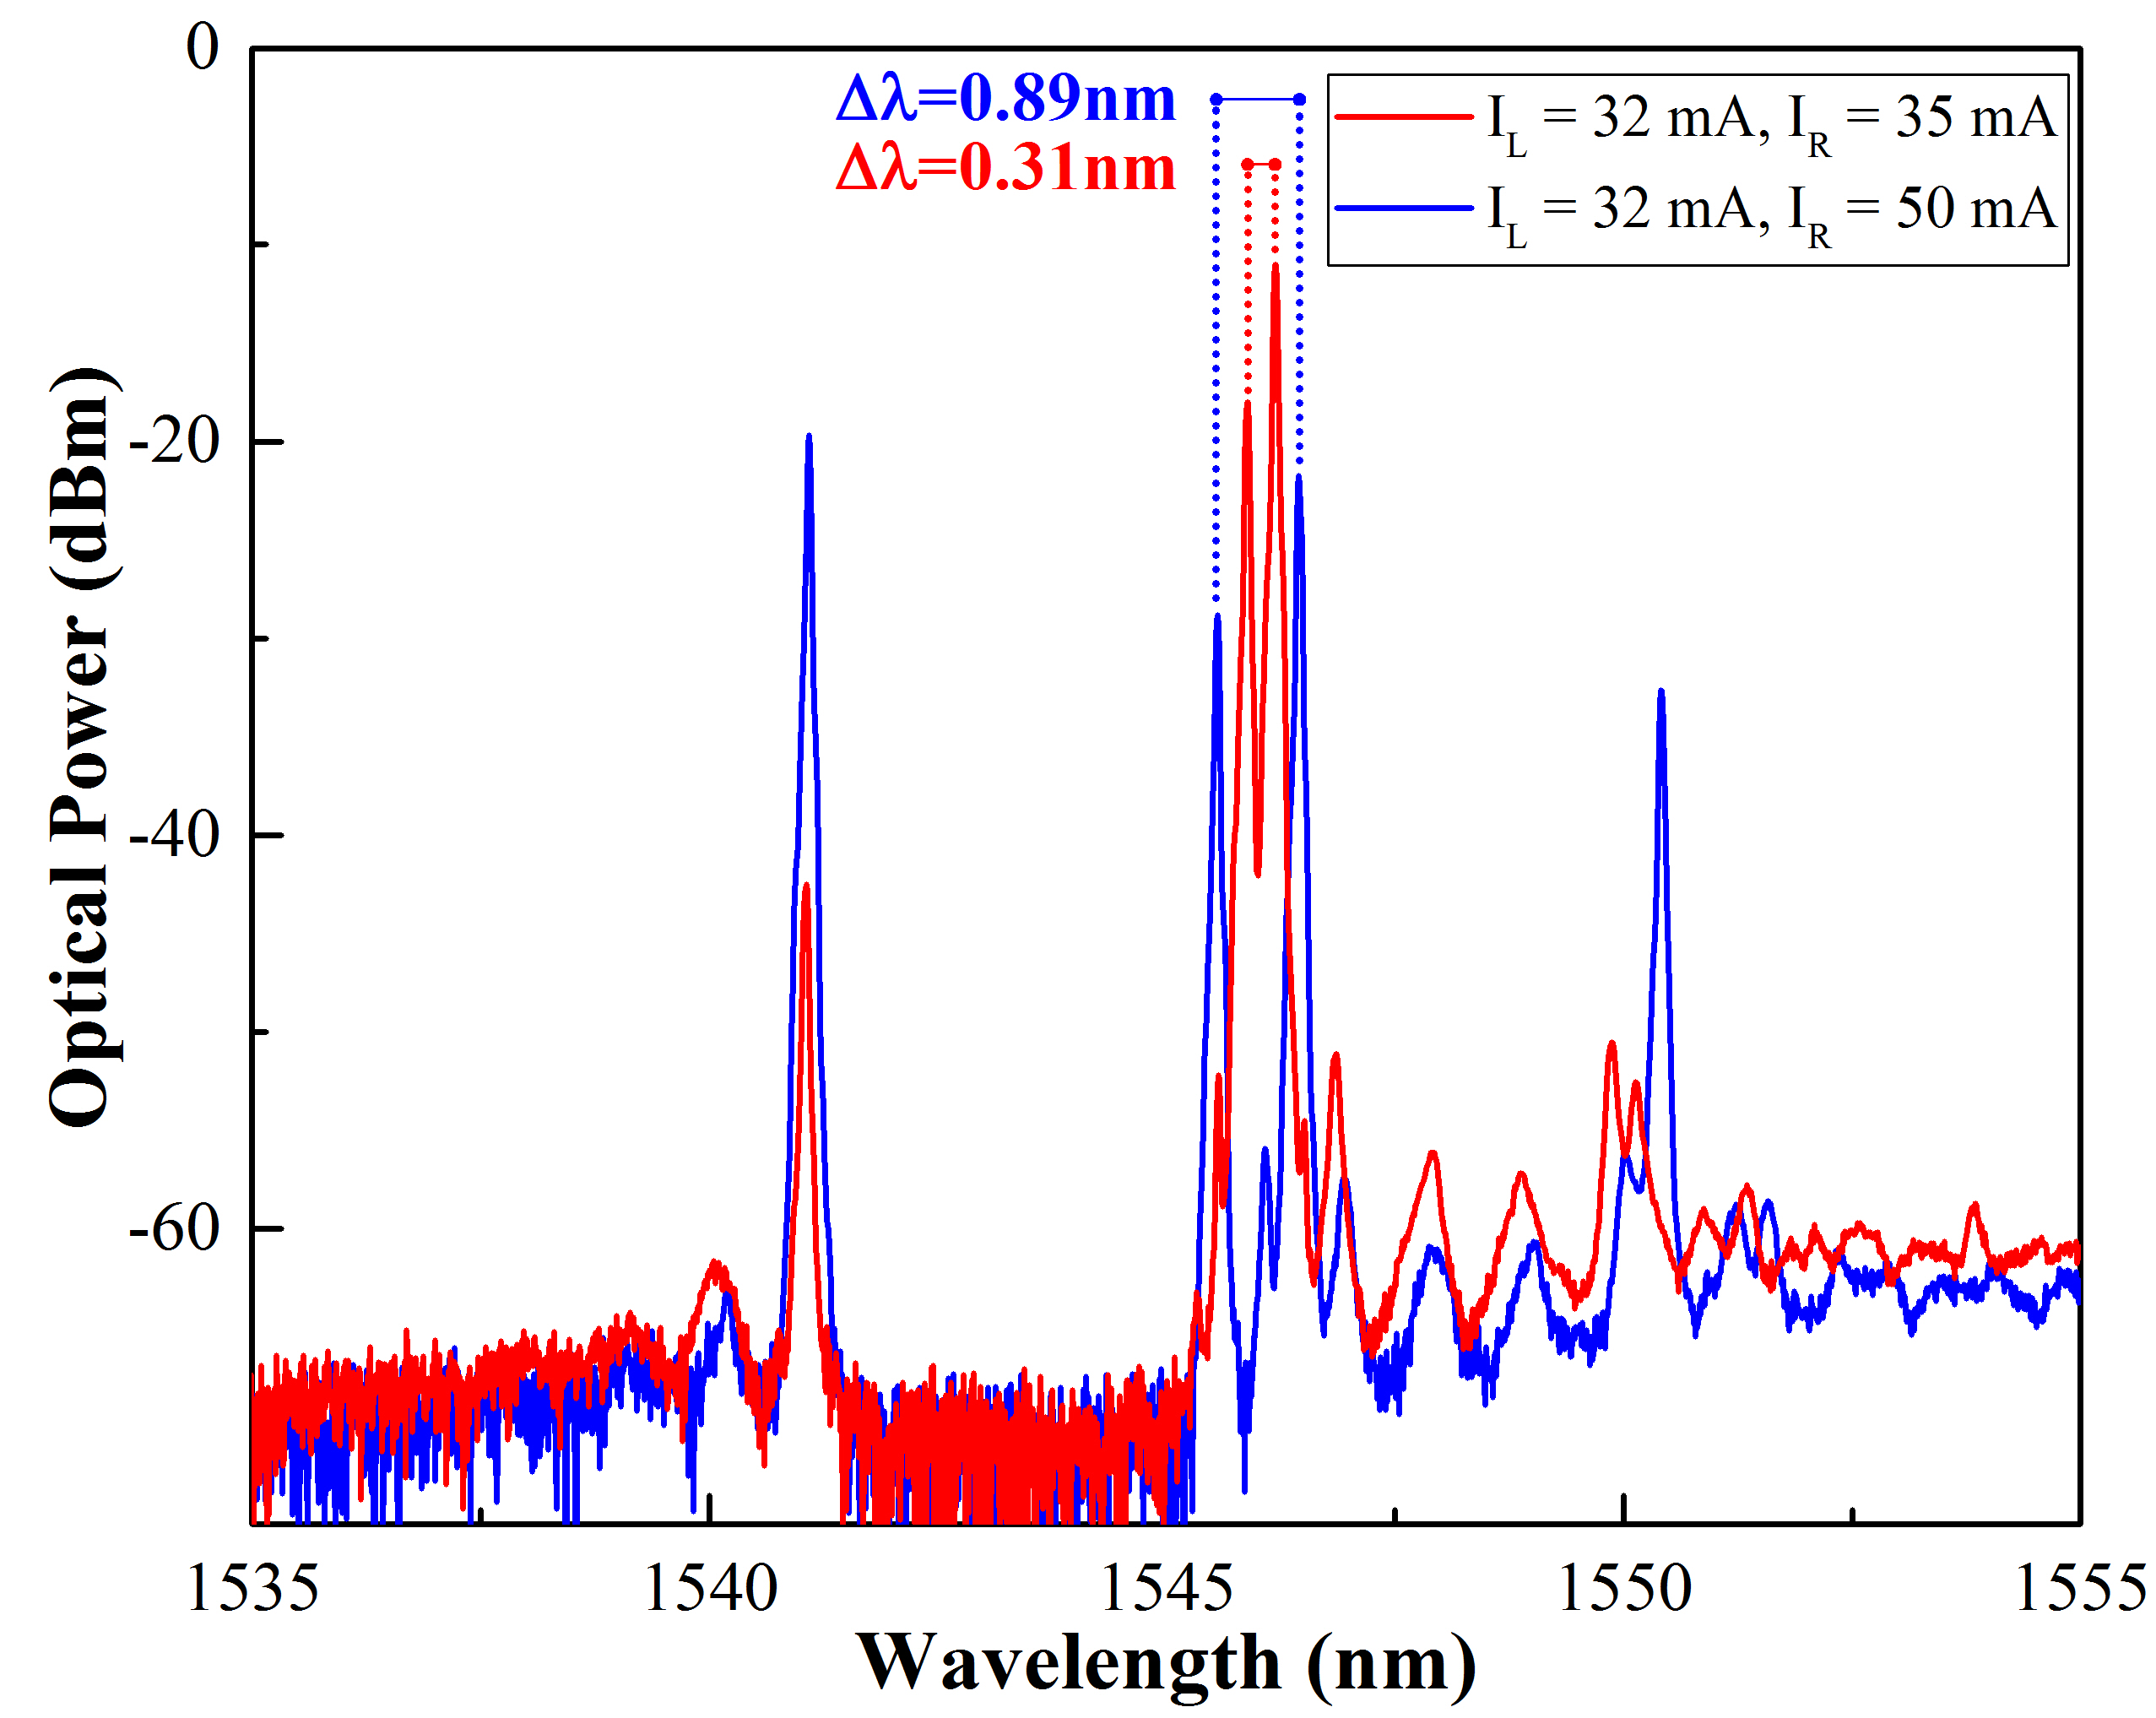
\includegraphics[width=12cm]{./Pictures/laser_spectrum.jpg}
	\captionsetup{justification=centering}
	\caption{两段式DFB激光器产生自脉冲时的光谱图}
	\label{laser_spectrum}
\end{figure}

我们研究了不同长度的激光器能够产生自脉冲的电流组合,如图\ref{laser_combination}所示,其中激光器的长度不包含两边锥形波导的长度。可以发现当激光器长度较短时,自脉冲出现后,往往固定一个电极的电流,改变另一个电极的电流能够保持自脉冲信号的存在,但当激光器的长度较长时,自脉冲出现后,我们需要将两段电流同时增大,才能保持自脉冲信号的存在。在两段式DFB激光器中,自脉冲出现的电流组合是分散式的,有些电流组合可能产生了激光器的频率锁定现象,无法产生拍频,导致无法观察到自脉冲信号;有些电流组合可能使得两个激射波长相距过大,其拍频超过了探测器的带宽,导致其无法响应。

\begin{figure}[htb]
	\centering
	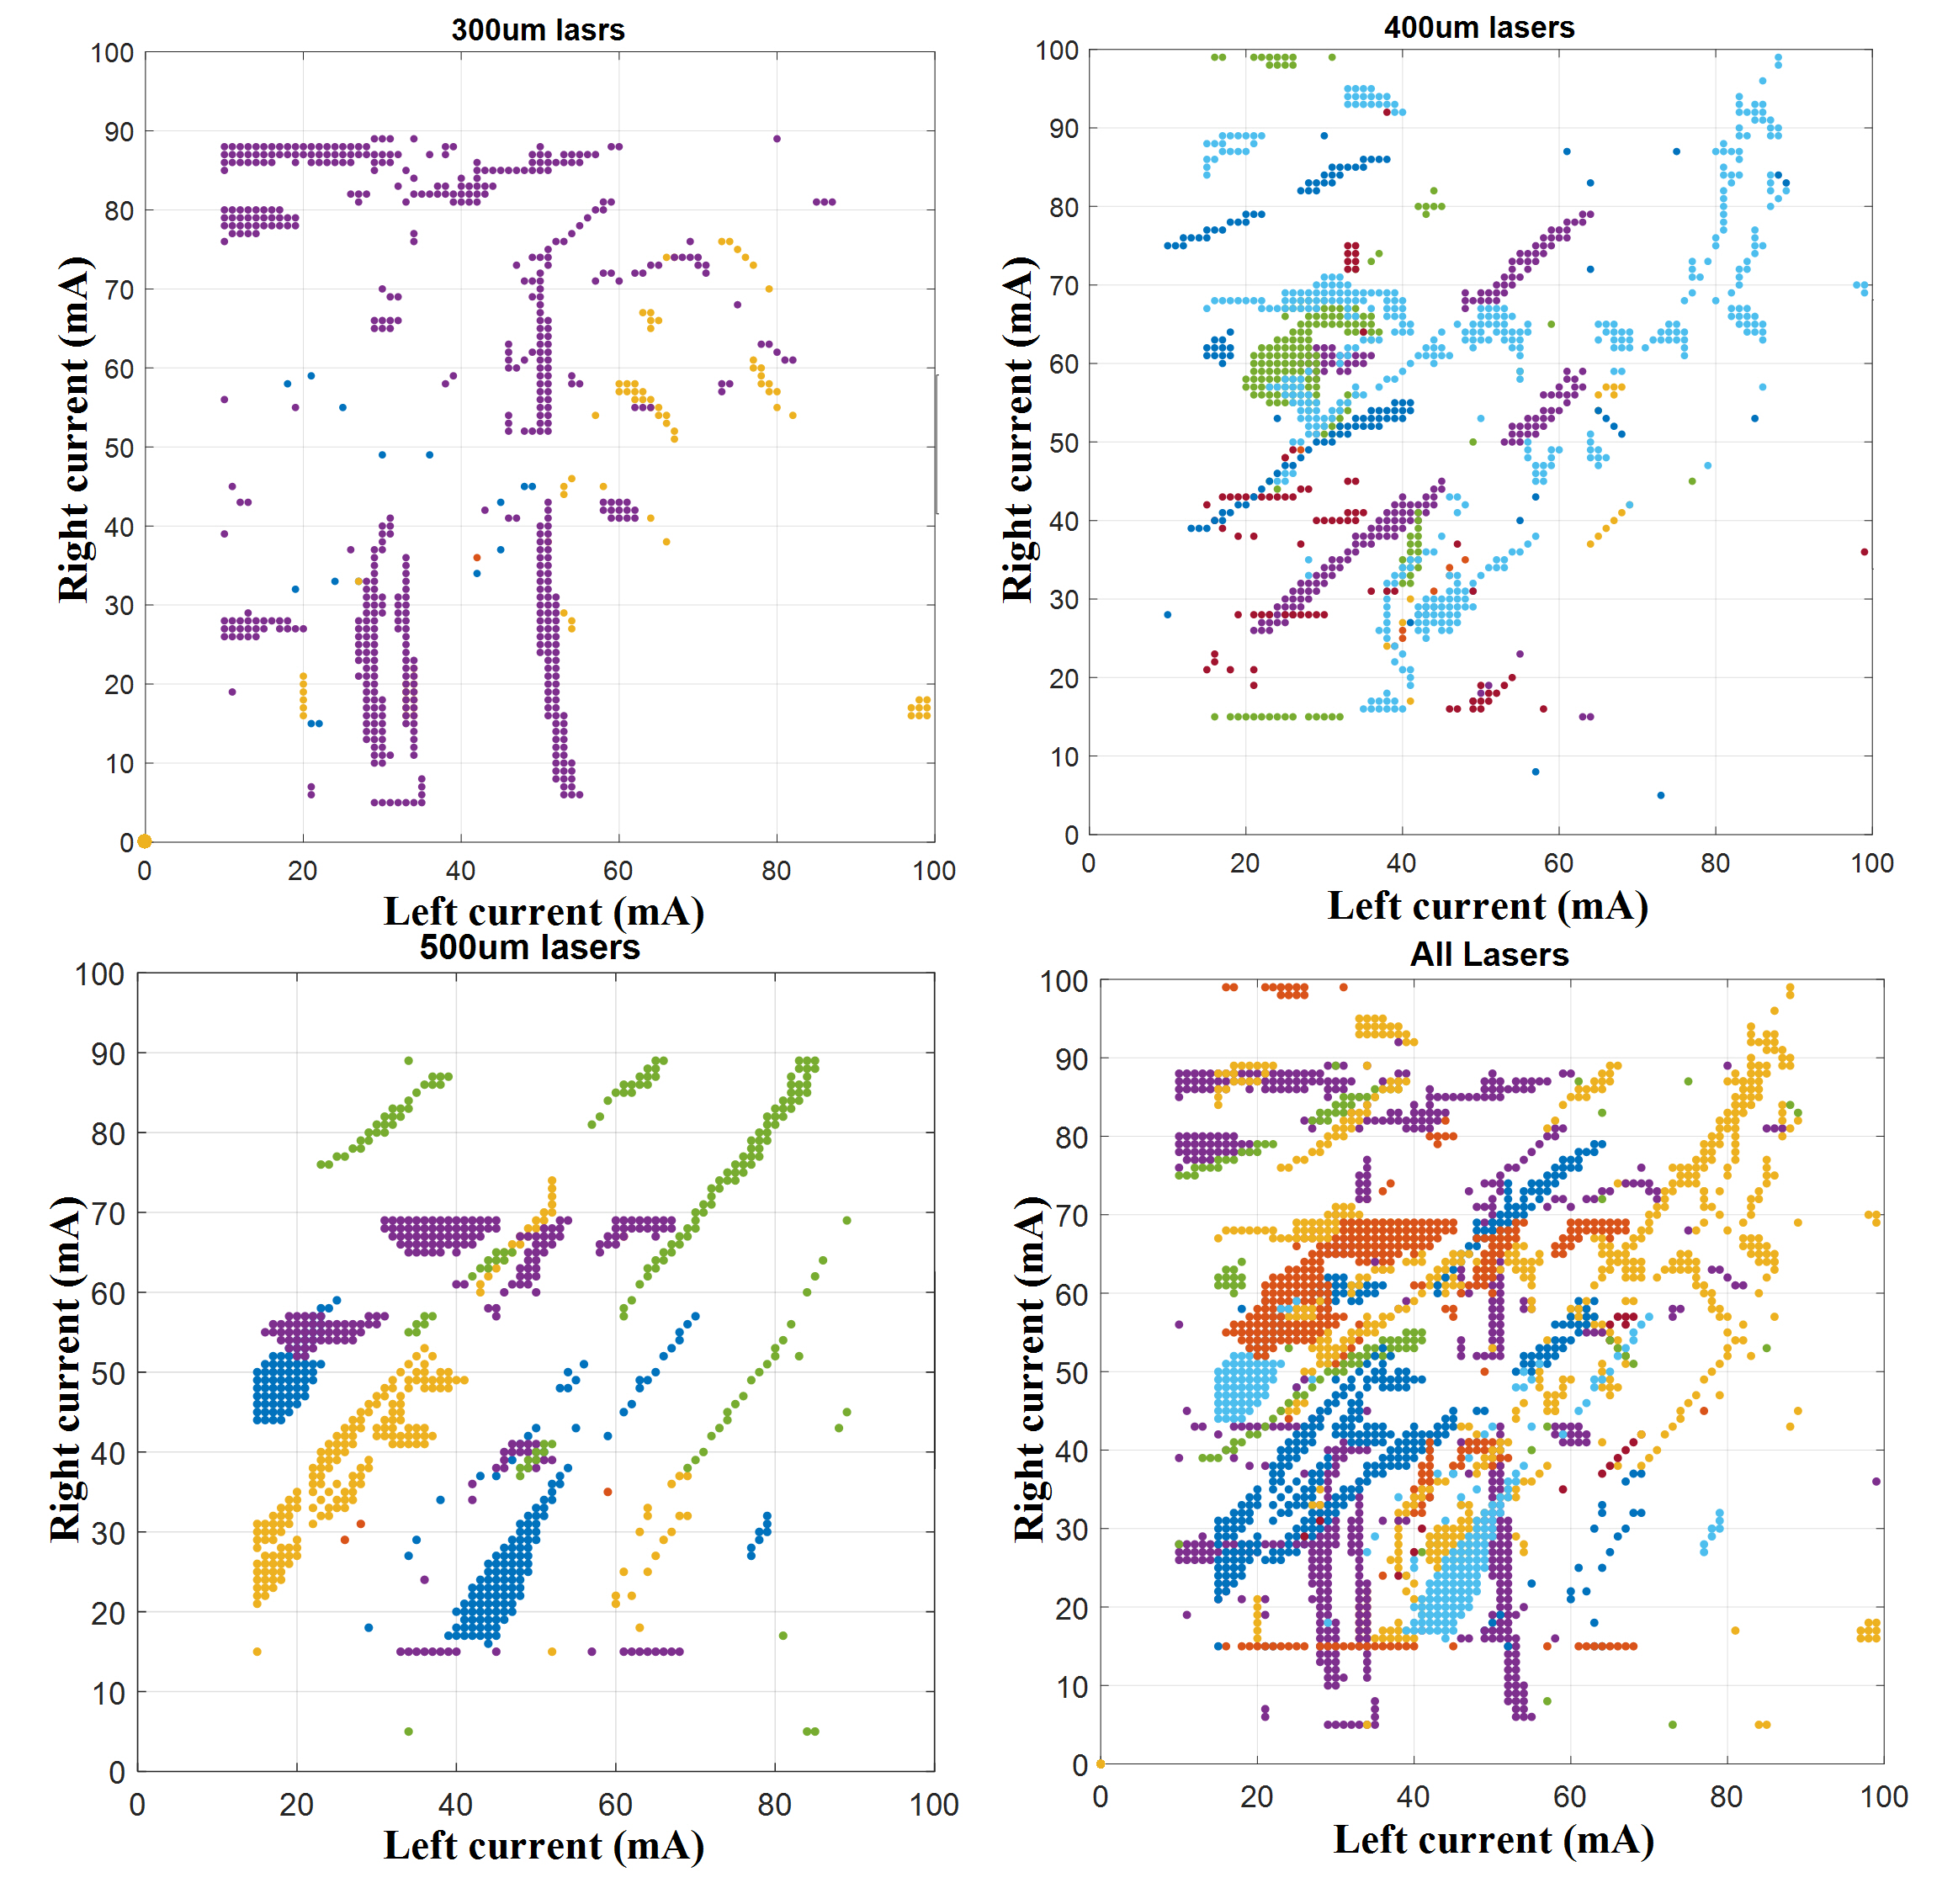
\includegraphics[width=15cm]{./Pictures/laser_combination.jpg}
	\captionsetup{justification=centering}
	\caption{不同长度的自脉冲DFB激光器电流组合,每个图中的不同颜色代表长度相同的不同激光器}
	\label{laser_combination}
\end{figure}

\begin{figure}[htb]
	\centering
	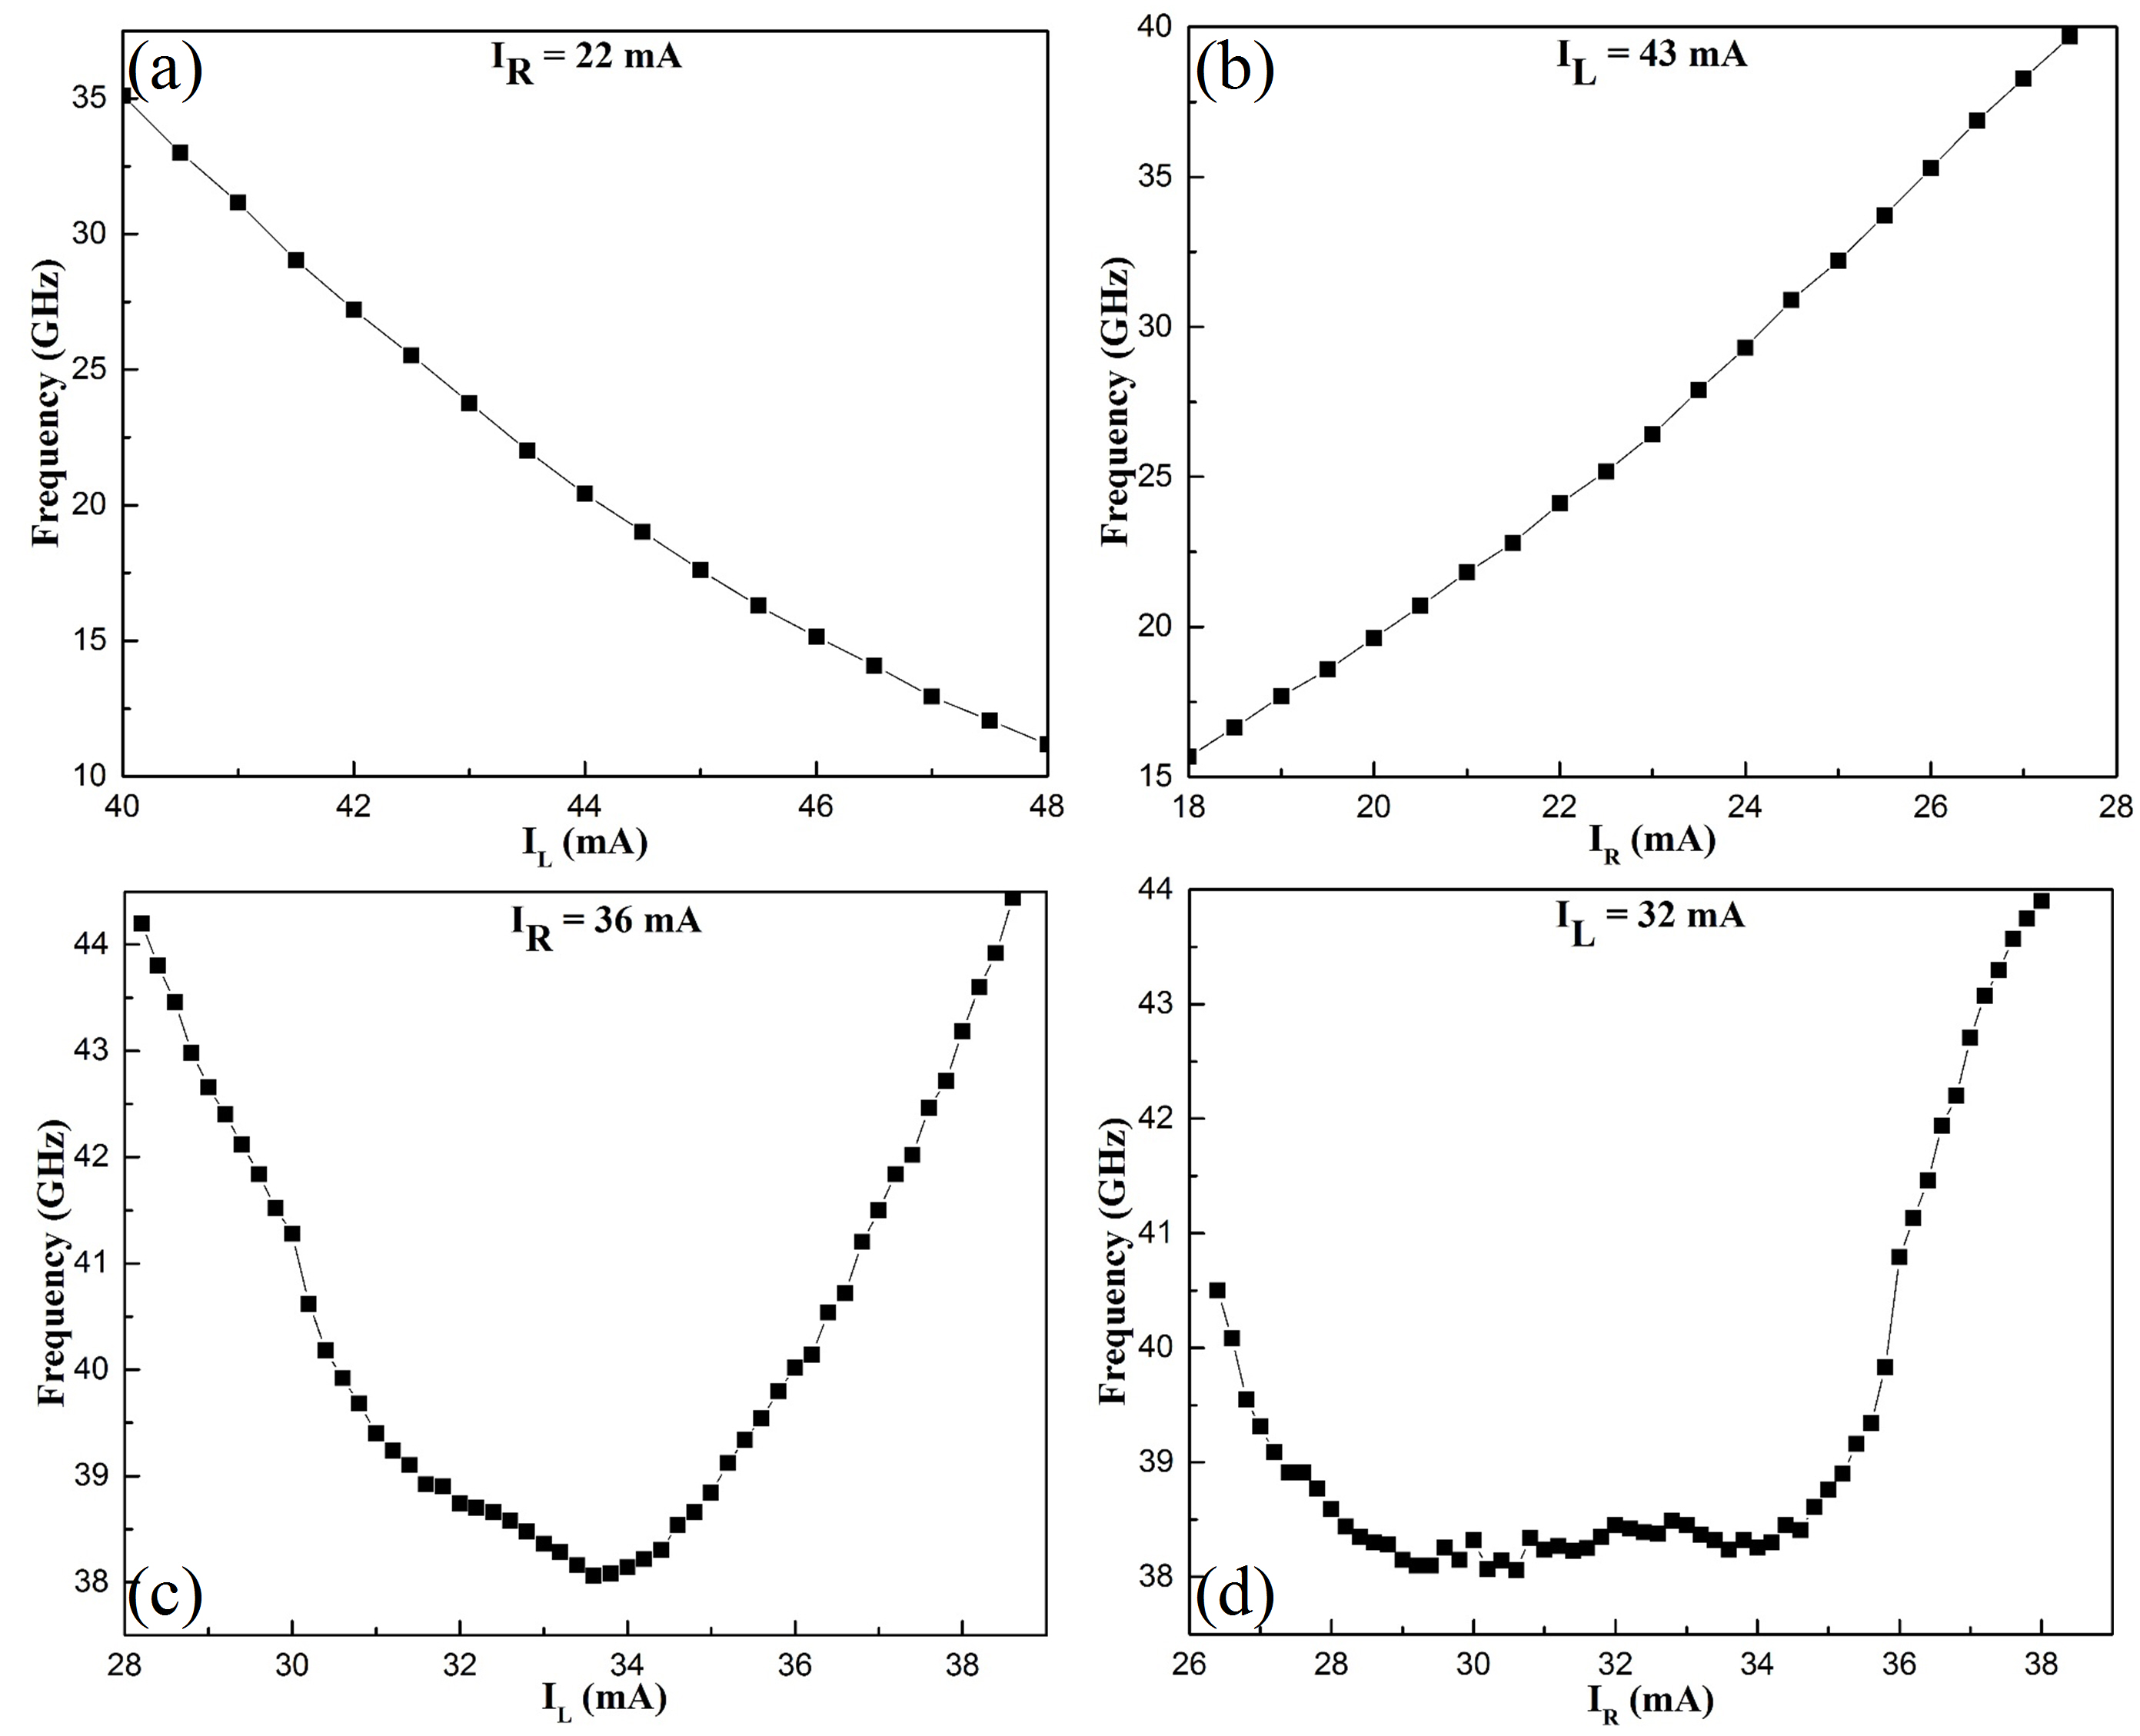
\includegraphics[width=15cm]{./Pictures/laser_self_pulsation.jpg}
	\captionsetup{justification=centering}
	\caption{自脉冲信号频率的电流调制,(a)(b)激光器A当其中一段泵浦电流固定时,自脉冲信号频率与另一段泵浦电流的关系;(c)(d)激光器B当其中一段泵浦电流固定时,自脉冲信号频率与另一段泵浦电流的关系}
	\label{laser_self_pulsation}
\end{figure}

我们研究了自脉冲信号频率与电流之间的关系,测试在15 $^{\circ}$C条件下进行,如图\ref{laser_self_pulsation}所示,其中图\ref{laser_self_pulsation}(a)、(b)中的双段式DFB激光器左段波导宽度为2~$\mu m$,右段波导宽度为4~$\mu m$,称之为激光器A,图\ref{laser_self_pulsation}(c)、(d)中的双段式DFB激光器左段波导宽度为2.5~$\mu m$,右段波导宽度为4~$\mu m$,称之为激光器B。从图\ref{laser_self_pulsation}(a)中可以看出,当激光器A右段电流I\SB{R} = 22 $mA$固定时,随着左段电流I\SB{L}增加,自脉冲信号的频率会相应的减小,可以实现25 GHz范围的频率调节。从图\ref{laser_self_pulsation}(b)中,我们可以看到相反的趋势,当激光器A左段电流I\SB{L} = 43 $mA$固定时,随着随着右段电流I\SB{R}增加,自脉冲信号的频率会相应的变大,也可以实现25~GHz范围的频率调节。但是并不是所有的激光器的自脉冲信号频率都显示出随电流线性变化的特性,我们可以看到图\ref{laser_self_pulsation}(c)、(d)中的激光器B,当其中一段电流固定时,改变另一段的电流,都会得到先减小后增大的自脉冲信号频率,中间还可能会有一段振荡的过程。

我们分析其中的原因,自脉冲信号频率的改变主要是通过改变激光器左右两段电流使激射波长发生改变,从而使得拍频信号产生变化。电流改变DFB激光器的波长,主要通过热效应来实现,因为当激光器处于激射状态时,载流子浓度不再发生改变。由于我们制作的激光器采用了应变量子阱材料,其可能包含增益杠杆效应\cite{vahala1989optical},该效应会影响载流子的分布。在图\ref{laser_self_pulsation}(a)、(b)中被电流调谐的激光器,热效应占主导地位,左段激光器的激射波长小于右段激光器。当增加左段激光器的泵浦电流时,热效应使得其激射波长往长波方向漂移,使得两段激光器的激射波长开始靠近,故自脉冲频率下降,漂移速度约为2.8~GHz$/K$,对应的波长漂移速度约为0.02~$nm/K$。而增加右边的电流,会使得两段激光器的激射波长远离,故自脉冲信号频率会增大;在图\ref{laser_self_pulsation}(c)、(d)中被电流调谐的激光器,左右两段激光器泵浦电流比较接近,改变某段激光器的注入电流可能会影响到另一段的载流子分布,可以看到,一旦当两段激光器的电流差别比较大时,自脉冲信号的频率就又开始单调变化了。

\begin{figure}[htb]
	\centering
	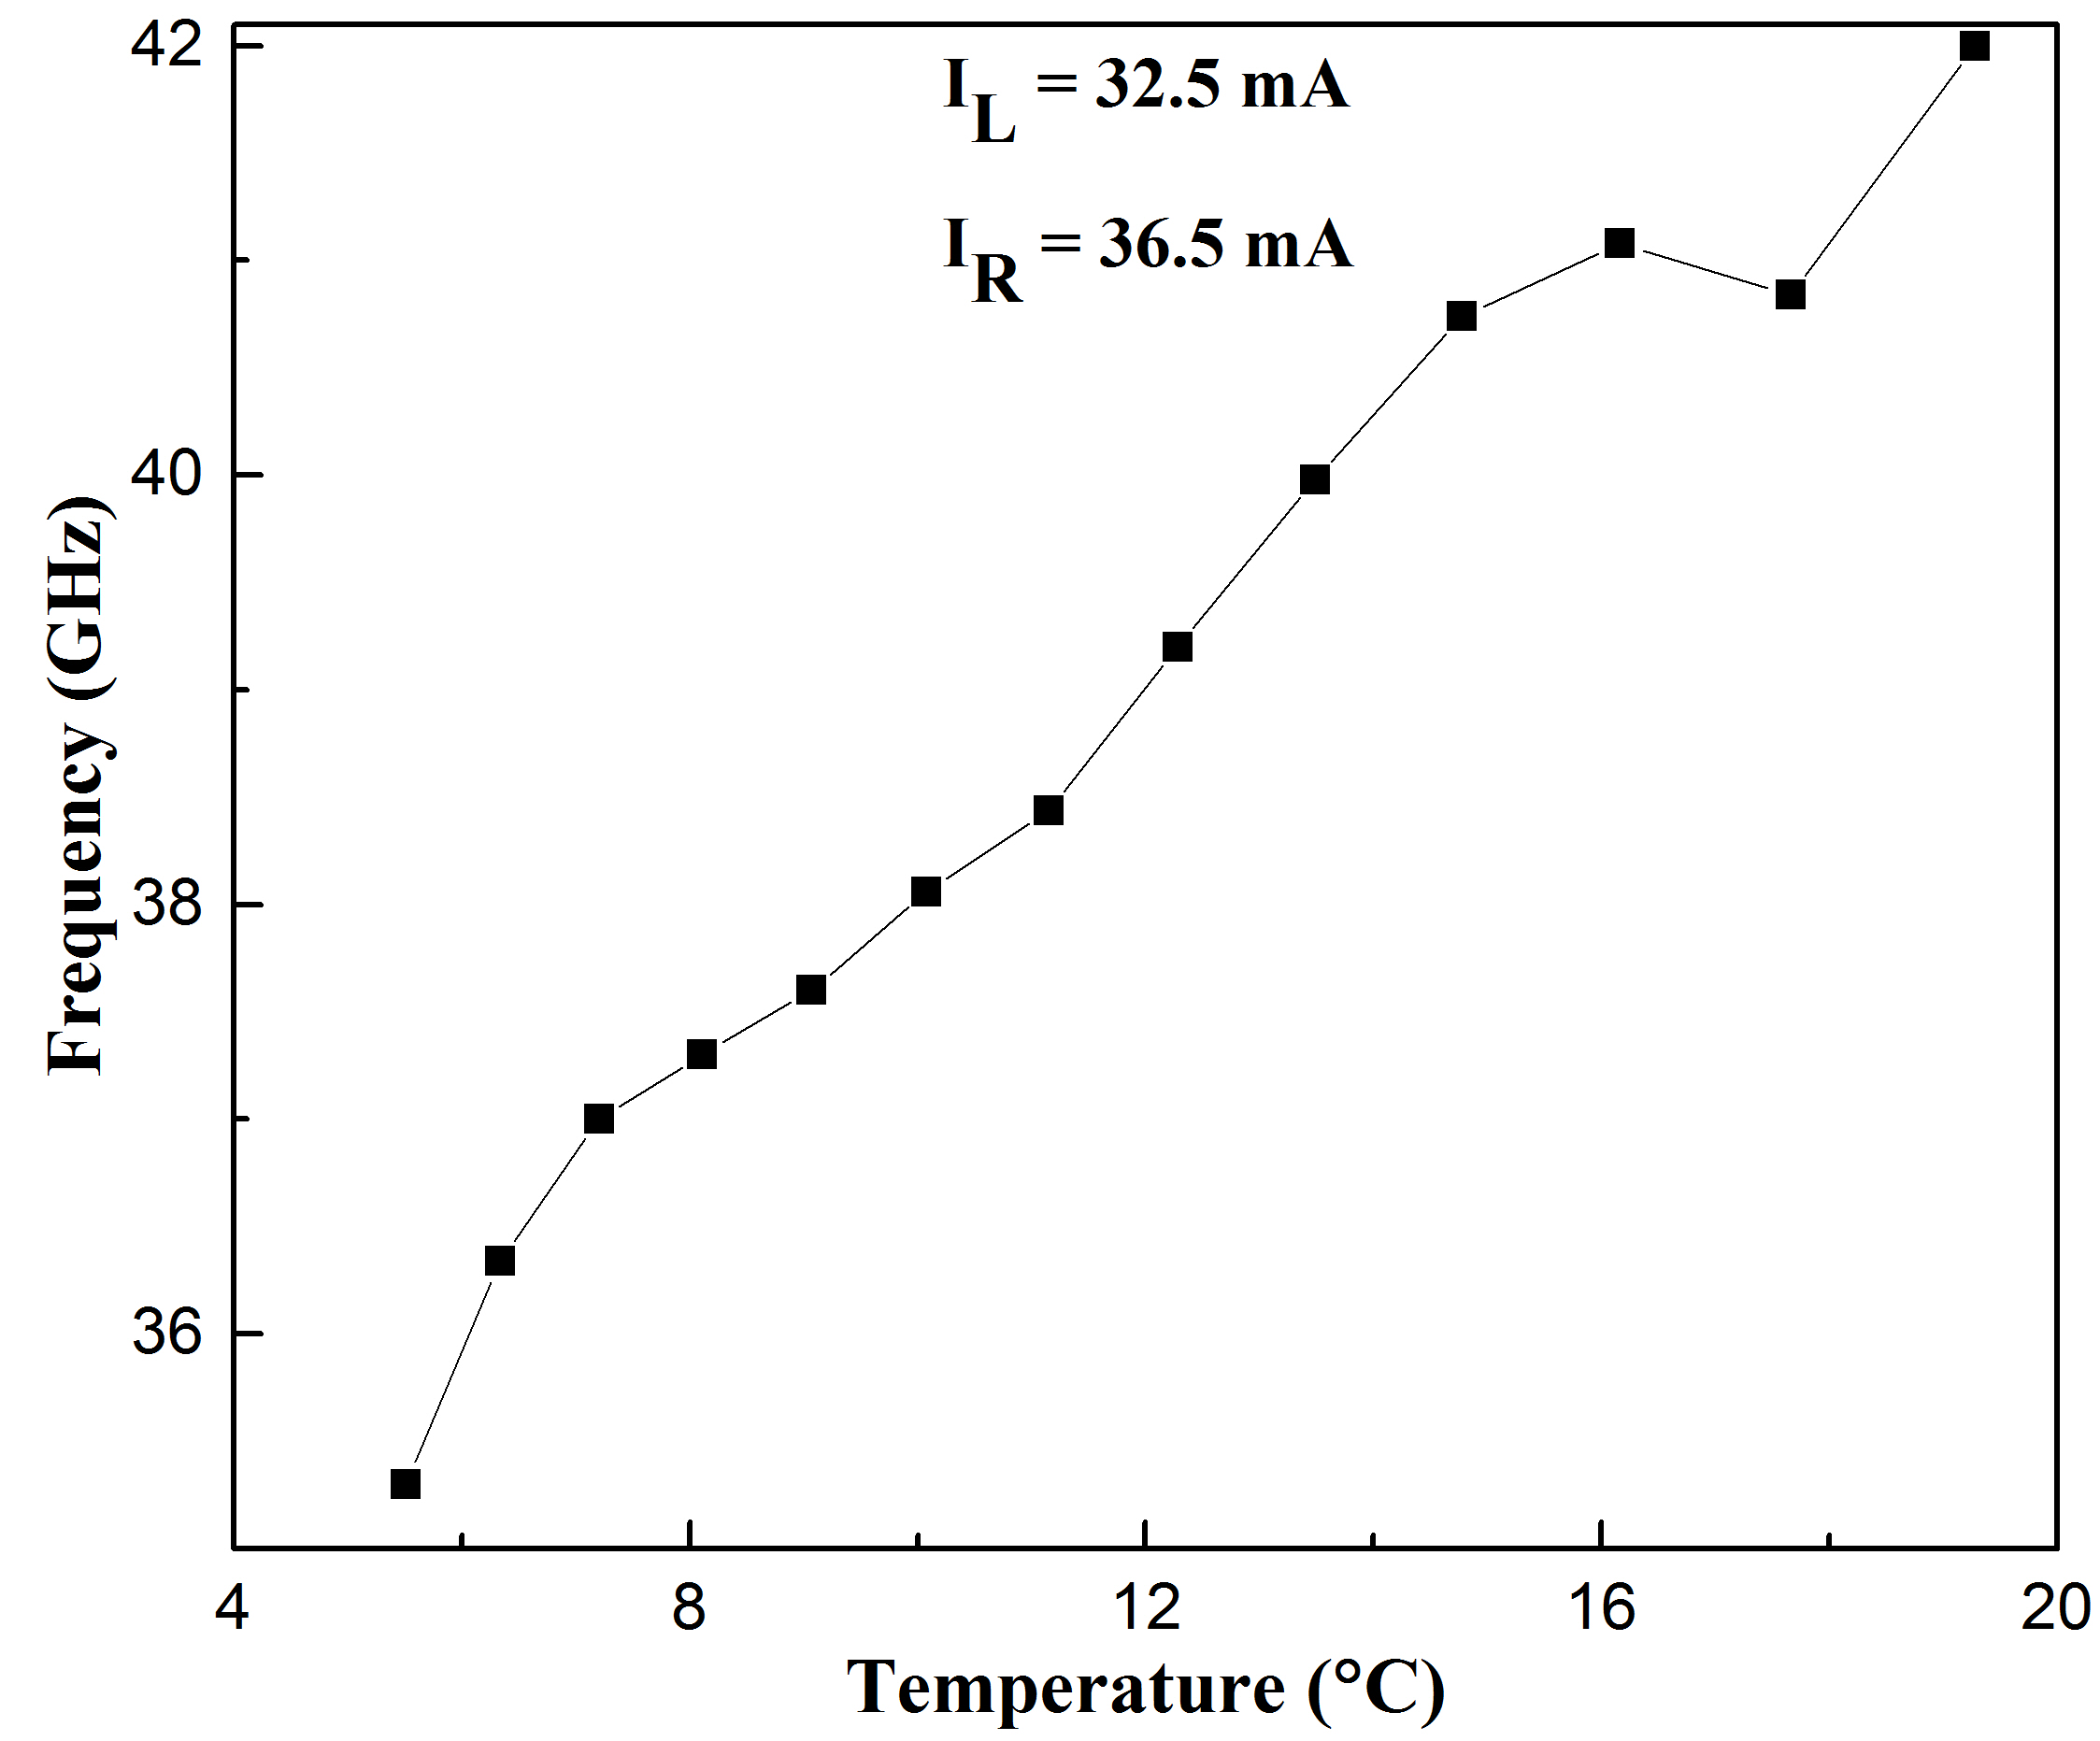
\includegraphics[width=12cm]{./Pictures/laser_temperature.jpg}
	\captionsetup{justification=centering}
	\caption{自脉冲信号频率与温度的关系}
	\label{laser_temperature}
\end{figure}

我们同样研究了温度对自脉冲信号频率的影响,如图\ref{laser_temperature}所示,可以看到随着温度升高,自脉冲频率也会变大,漂移速度约为1.9~GHz$/K$。

\begin{figure}[htb]
	\centering
	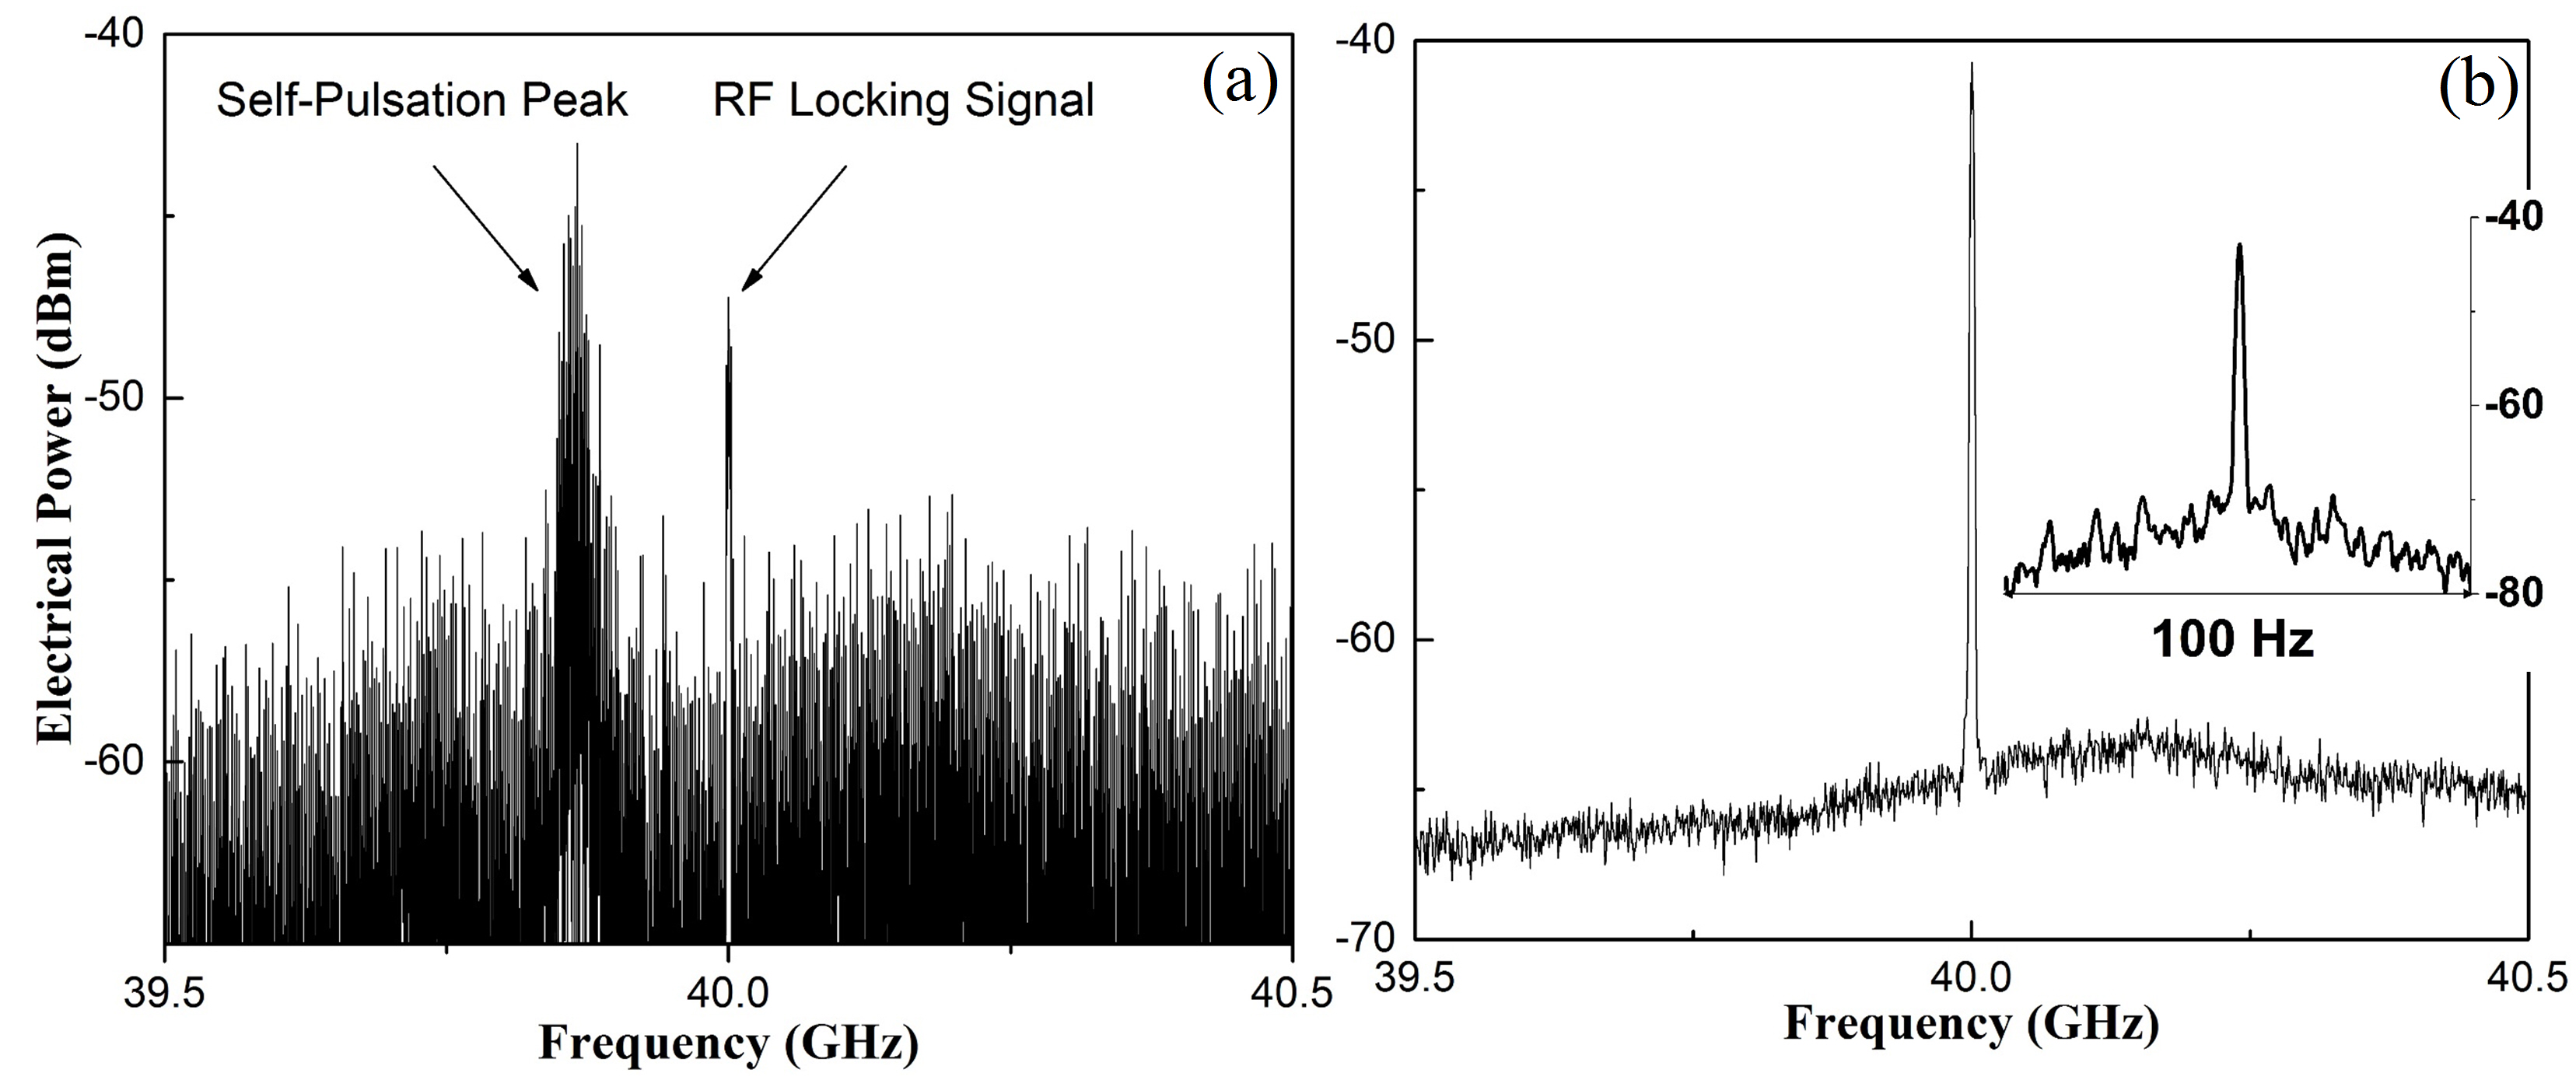
\includegraphics[width=15cm]{./Pictures/laser_lock.jpg}
	\captionsetup{justification=centering}
	\caption{两段式自脉冲DFB激光器的频率锁定现象,(a)未锁定状态;(b)锁定状态,插图为自脉冲信号测试时的放大图}
	\label{laser_lock}
\end{figure}

我们还发现了自脉冲信号的锁定现象如图\ref{laser_lock}所示,这可以用来产生窄带光学微波信号。实验时用外置微波信号源通过高速探针将微波信号加载到自脉冲激光器其中一段上,当微波信号频率离自脉冲信号频率相差较远的时候,两者互相不受影响,如图\ref{laser_lock}(a)所示,此时自脉冲信号的线宽为几十MHz,这是由两段激光器的相位噪声决定所决定。但当微波信号处于自脉冲信号的带宽范围内时,激光器的自脉冲信号会被锁定到微波信号的频率上,我们得到的锁定最小微波功率为-17~dBm,且其自脉冲信号线宽可以小于10~Hz,如图\ref{laser_lock}(b)所示。该现象可以这样解释:当微波信号加载到某一段激光器上时,会通过注入锁定现象使得该段激光器的相位与注入的微波信号保持一致,该段激光器相位噪声变小,同时产生调制边带,边带的频率与激光器的中心频率之差为所加载的微波信号频率大小。该段激光器输出的调制边带又通过注入锁定使得另一段激光器的相位也被锁定,所不同的是,前者是电信号的注入锁定,后者是光信号的注入锁定。经过锁定之后,拍频产生的自脉冲信号相位噪声也几乎消失,所以能够得到非常纯净的光学微波信号。

\section{自脉冲激光器的动态调制性能}

如第一章中所介绍的,光收发模块中的调制方式有两种,一种是利用激光器输出功率恒定的激光,由外接调制器对其光强等参数进行调制的外调制方式,该种调制方式不受啁啾效应\cite{wakita1991observation}的影响,产生的信号可以用于长距离的光纤传输,但其缺点也正因为多了一个调制器,故整个光发射机尺寸、能耗都有所增大,而且由于要考虑激光器与调制器之间的耦合以及调制器的插损,发射机对激光器输出功率的要求也会高一点;另一种调制方式是通过调制激光器驱动电流的直接调制方式,该种调制方式能耗会比较低,但是其调制速带宽往往受限于载流子与光子的弛豫振荡频率,调制速率往往没有外调的方式快,而且在进行光强调制时,往往会伴随着频率啁啾的现象,使得信号在光纤中传输时色散效应加重,故直接调制比较适合用于短距离的数据传输。

\subsection{自脉冲激光器的调制带宽}

\begin{figure}[htb]
	\centering
	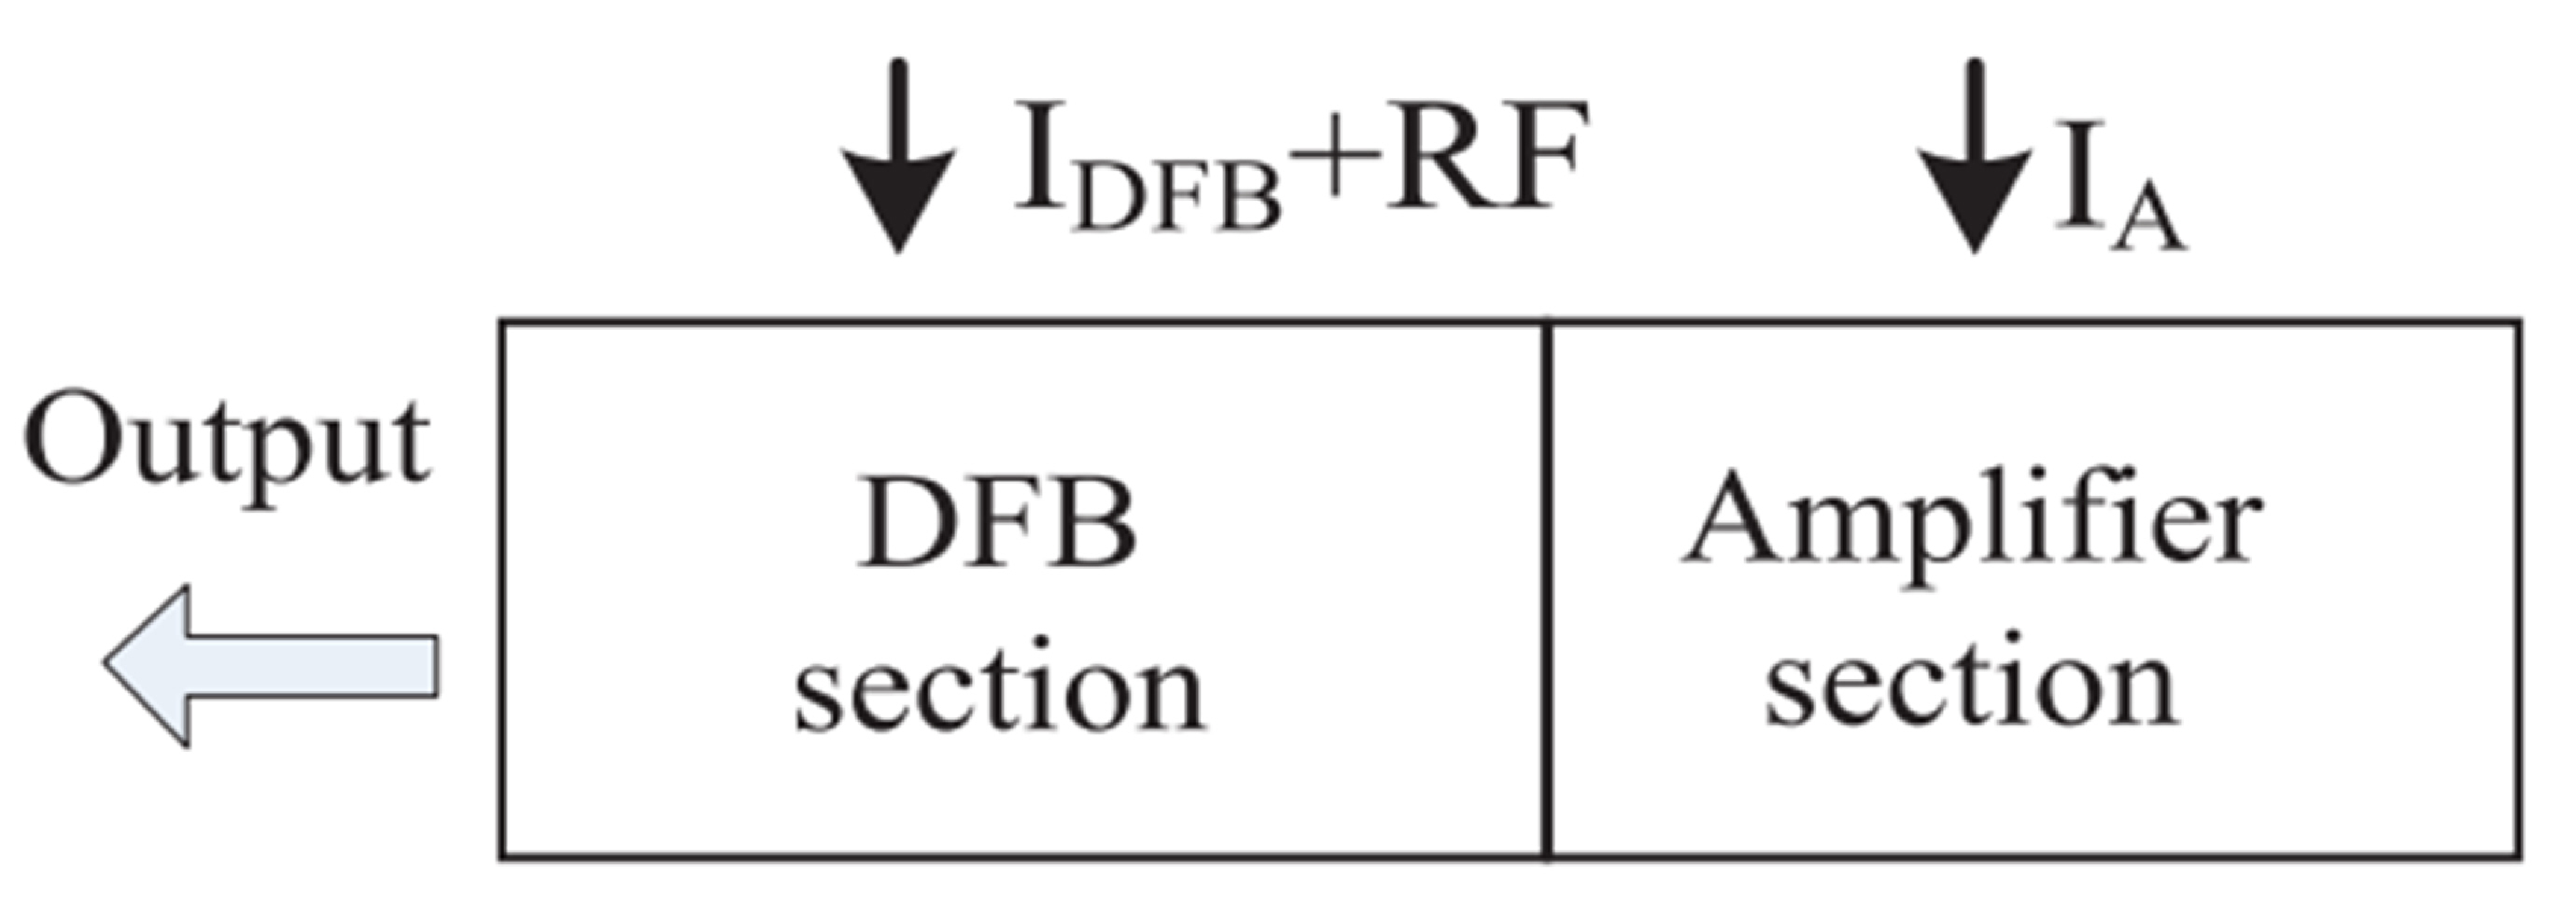
\includegraphics[width=13cm]{./Pictures/laser_ppr_structure.jpg}
	\captionsetup{justification=centering}
	\caption{耦合腔双波长激光器示意图\cite{wei2016realizing}}
	\label{laser_ppr_structure}
\end{figure}

\begin{figure}[htb]
	\centering
	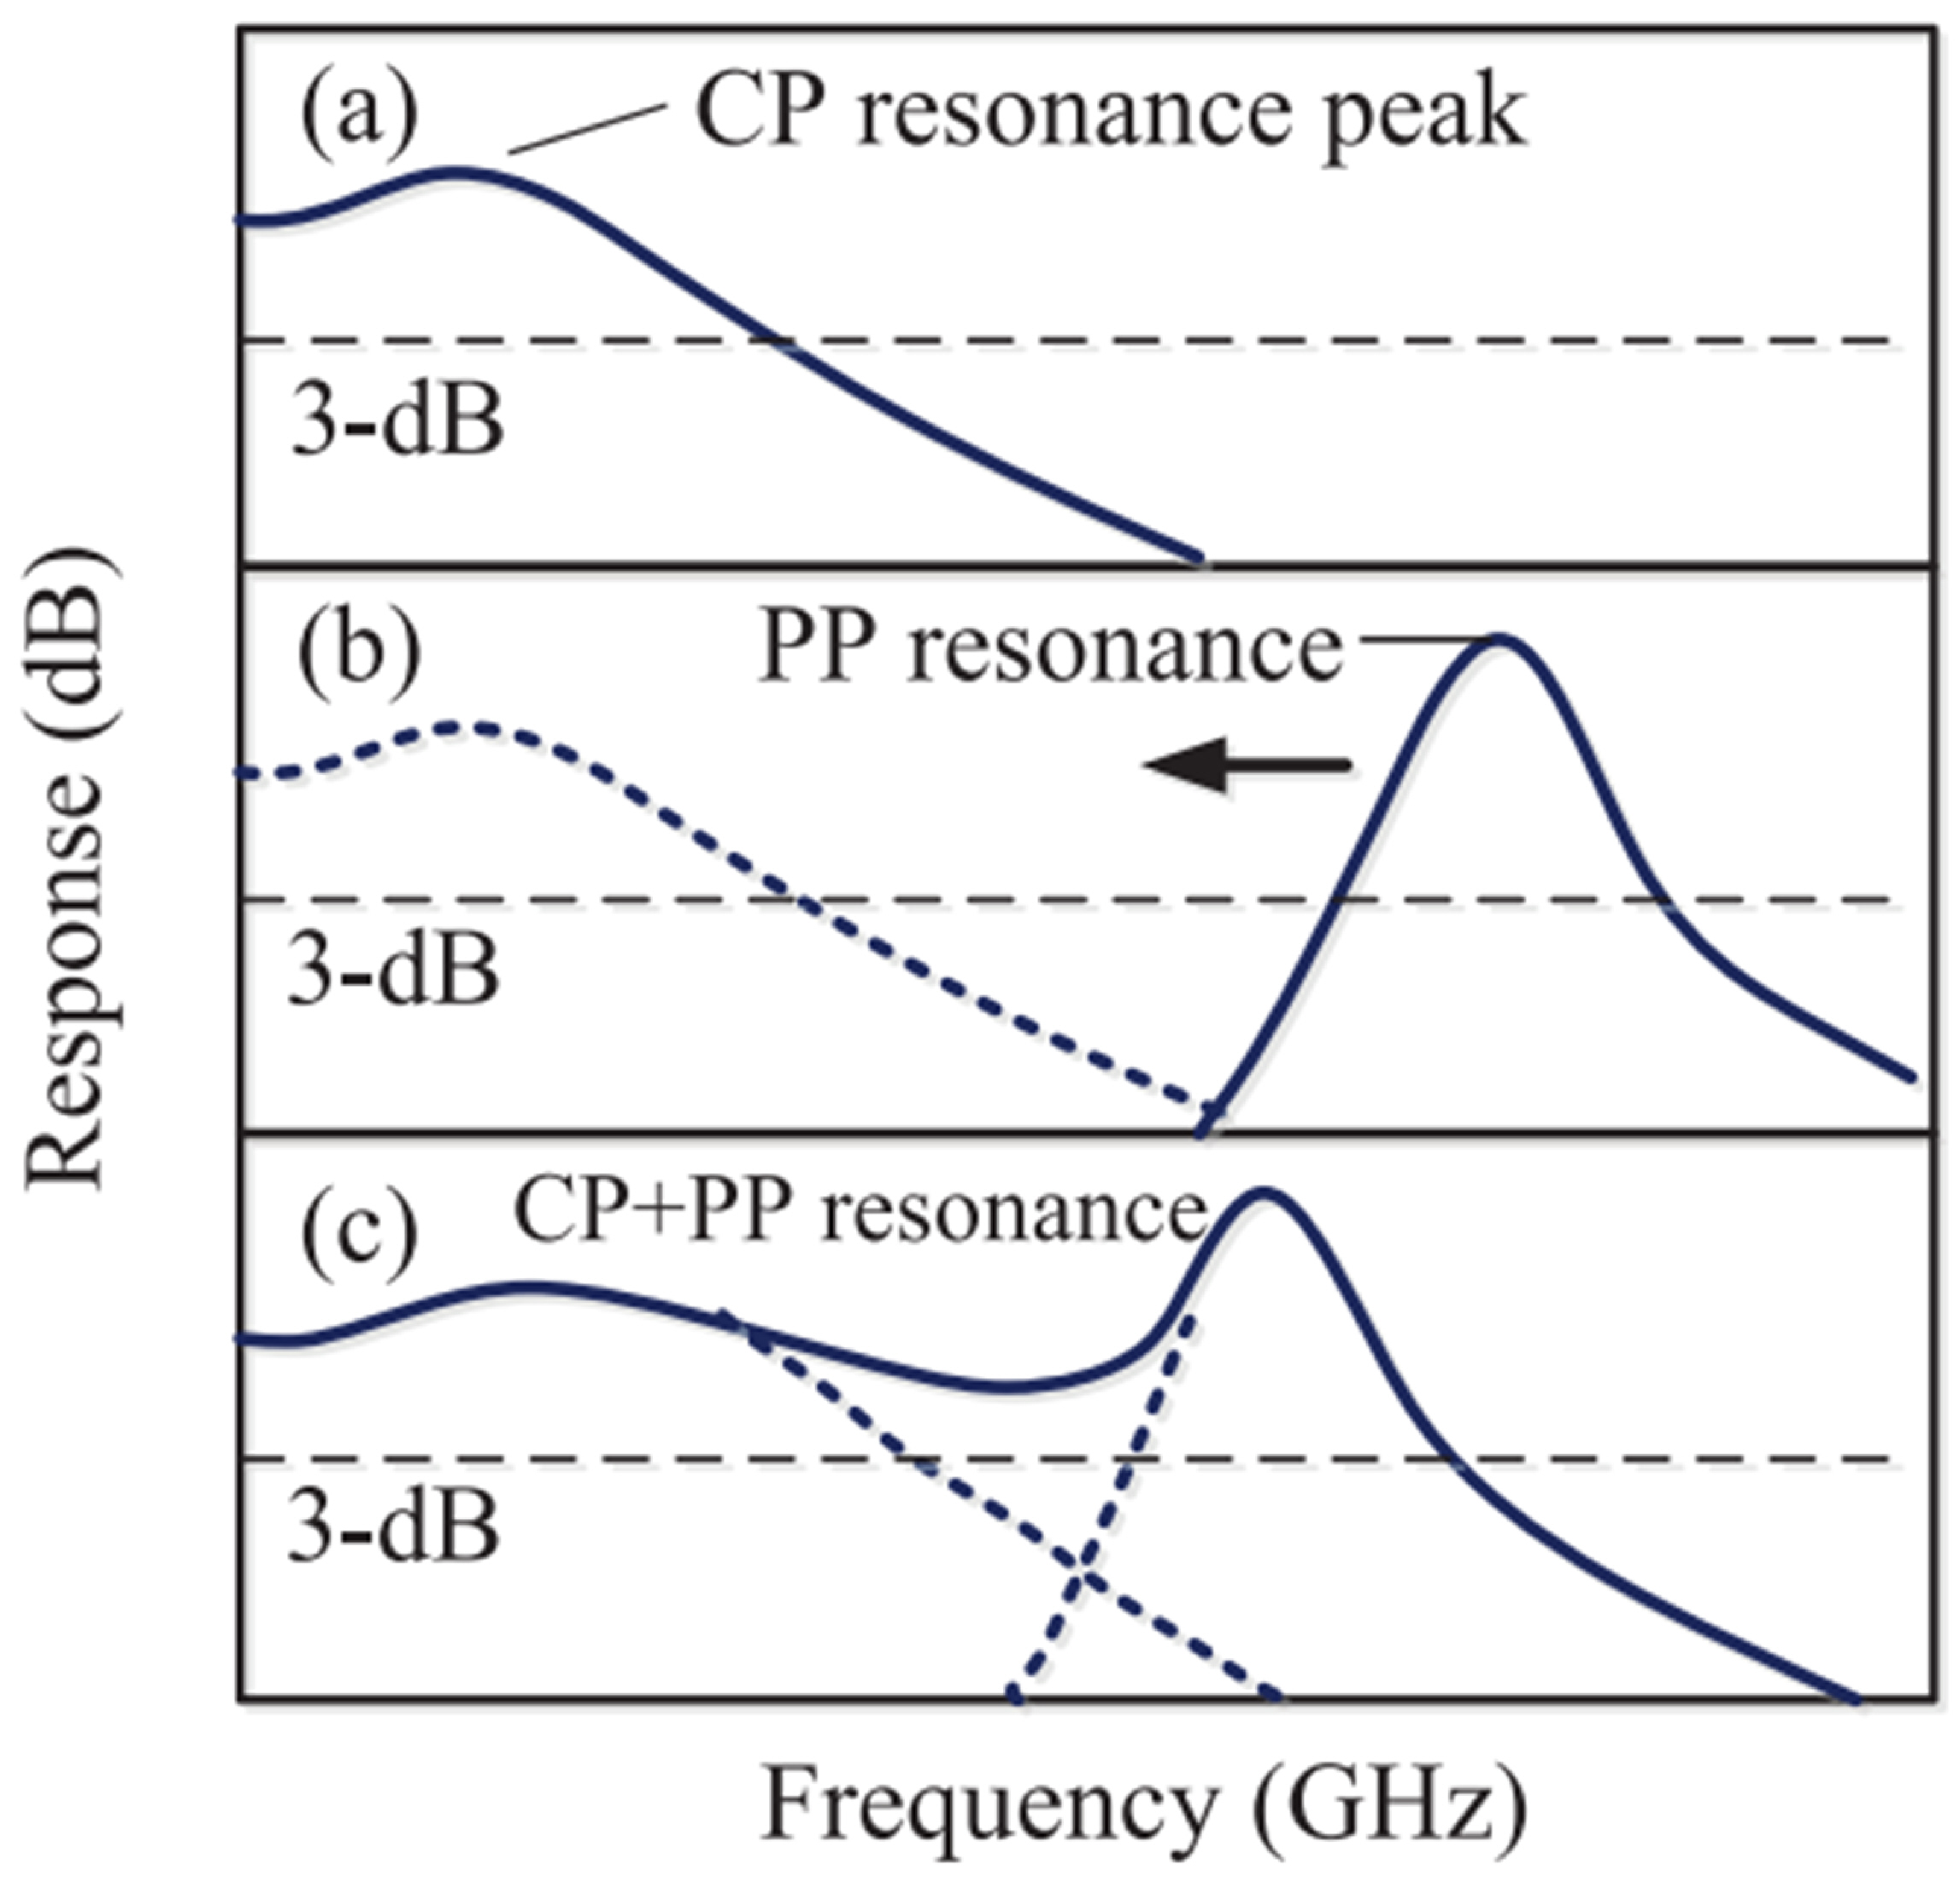
\includegraphics[width=12cm]{./Pictures/laser_ppr.jpg}
	\captionsetup{justification=centering}
	\caption{耦合腔双波长激光器的调制响应,(a)只有弛豫振荡峰;(b)光子共振峰远离弛豫振荡峰;(c)光子共振峰与弛豫振荡峰相距适中\cite{wei2016realizing}}
	\label{laser_ppr}
\end{figure}

耦合腔激光器中的光子共振现象(photon-photon resonance, PPR)可以增加激光器的调制带宽,且可以有多种不同的实现方案,比如双段式DFB激光器\cite{wenzel1996mechanisms},耦合腔注入激光器\cite{reithmaier2005modulation},有源反馈激光器\cite{brox2003high}和无源反馈激光器\cite{tager1994high}。如图\ref{laser_ppr_structure}所示为一个耦合腔双波长激光器的示意图,该激光器由两部分构成,一部分为DFB光栅区域,另一部分为增益区,两者构成了一个耦合腔系统。如第二章所述,对于一个普通的DFB激光器,其调制带宽往往受到弛豫振荡频率的限制,如图\ref{laser_ppr}(a)所示。对基于InGaAsP材料作为量子阱材料制作的DFB激光器来说,其弛豫振荡频率往往在10 GHz以下,对基于InAlGaAs材料作为量子阱制作的DFB激光器来说,其弛豫振荡频率会高一点,但是一般也不超过15 GHz。但是,该耦合腔双波长激光器可以利用两个波长距离很近的模式之间的拍频来实现调制带宽的提升,该原理也是基于光子共振的现象,光子共振的频率由两个波长的频率差值决定。如图\ref{laser_ppr}(b)所示,当两波长相距较远,光子共振频率较大,与弛豫振荡频率相隔较远,无法提升激光器的调制带宽。当通过调整两波长之间的间距,使得光子共振频率与弛豫振荡频率相距适中,则当调制速率因超过驰豫振荡频率响应下降时,又通过光子共振频率得到补偿,则此时该激光器的调制响应会具有更大的带宽,如图\ref{laser_ppr}(c)所示。

我们制作的自脉冲DFB激光器也可以利用光子共振的效应来提升激光器的调制带宽,而且其可以通过调节左右两个电极的注入电流大小方便地控制左右两段激光器中的激射波长,从而控制光子共振频率的大小。

\begin{figure}[htb]
	\centering
	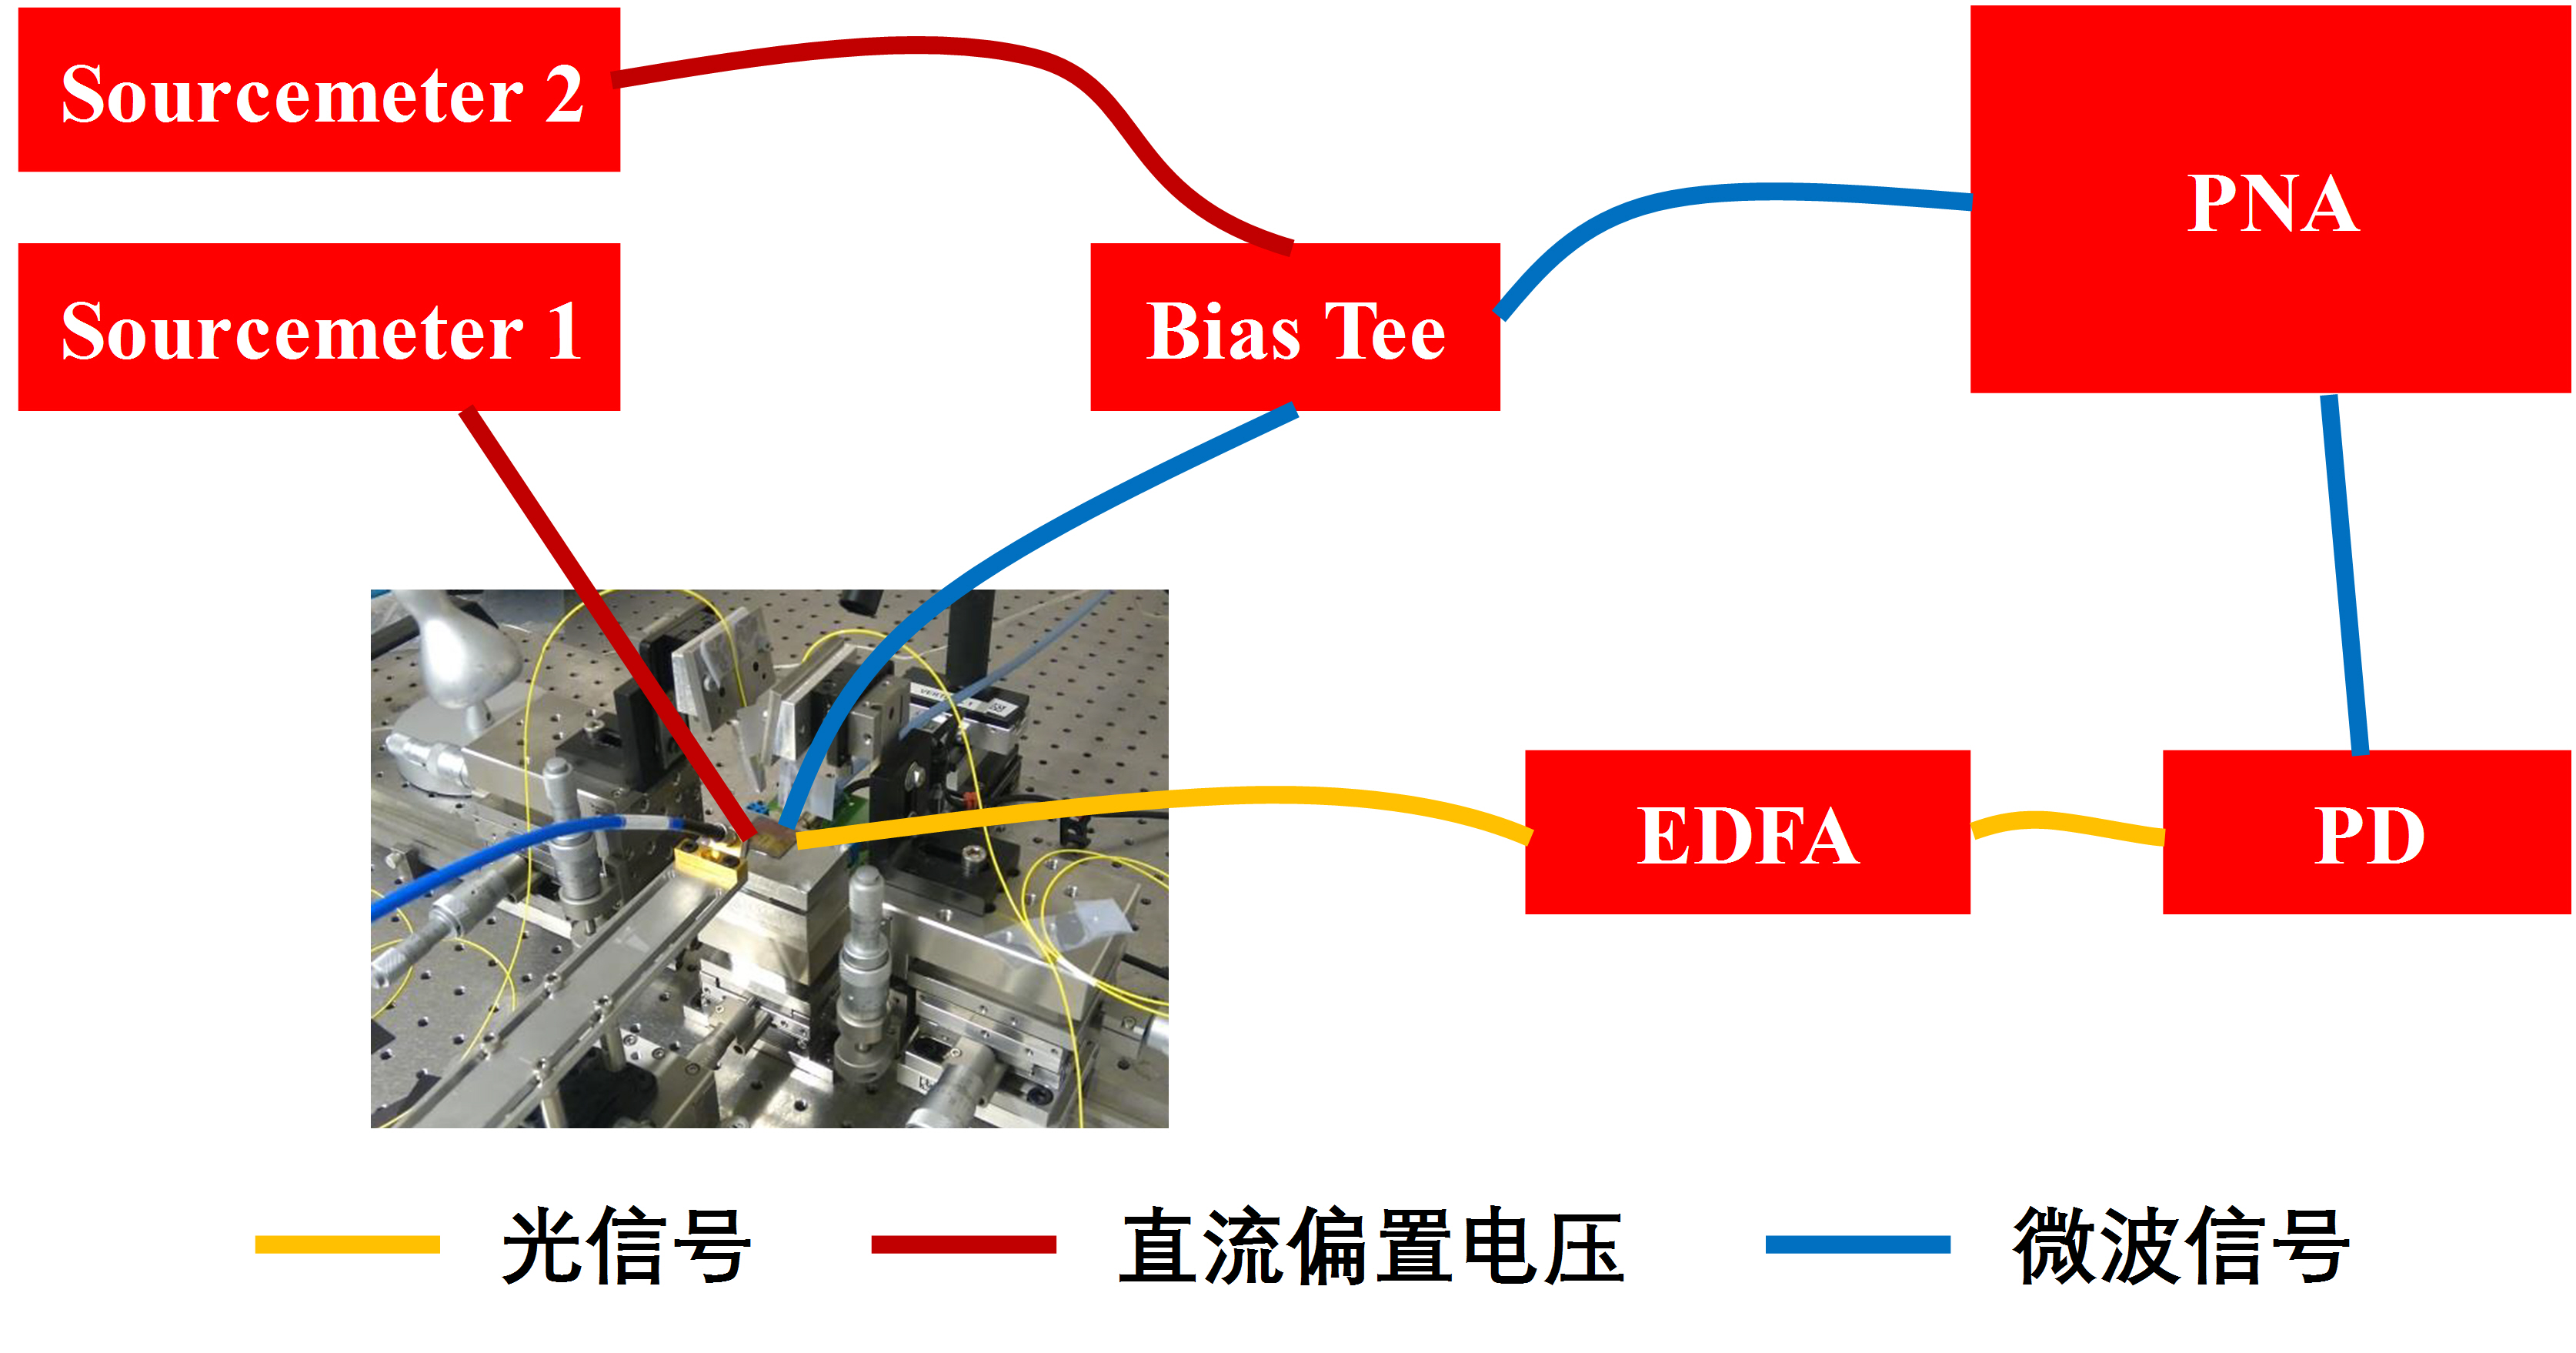
\includegraphics[width=15cm]{./Pictures/laser_s21_setup.jpg}
	\captionsetup{justification=centering}
	\caption{自脉冲激光器调制带宽测试示意图}
	\label{laser_s21_setup}
\end{figure}

\begin{figure}[htb]
	\centering
	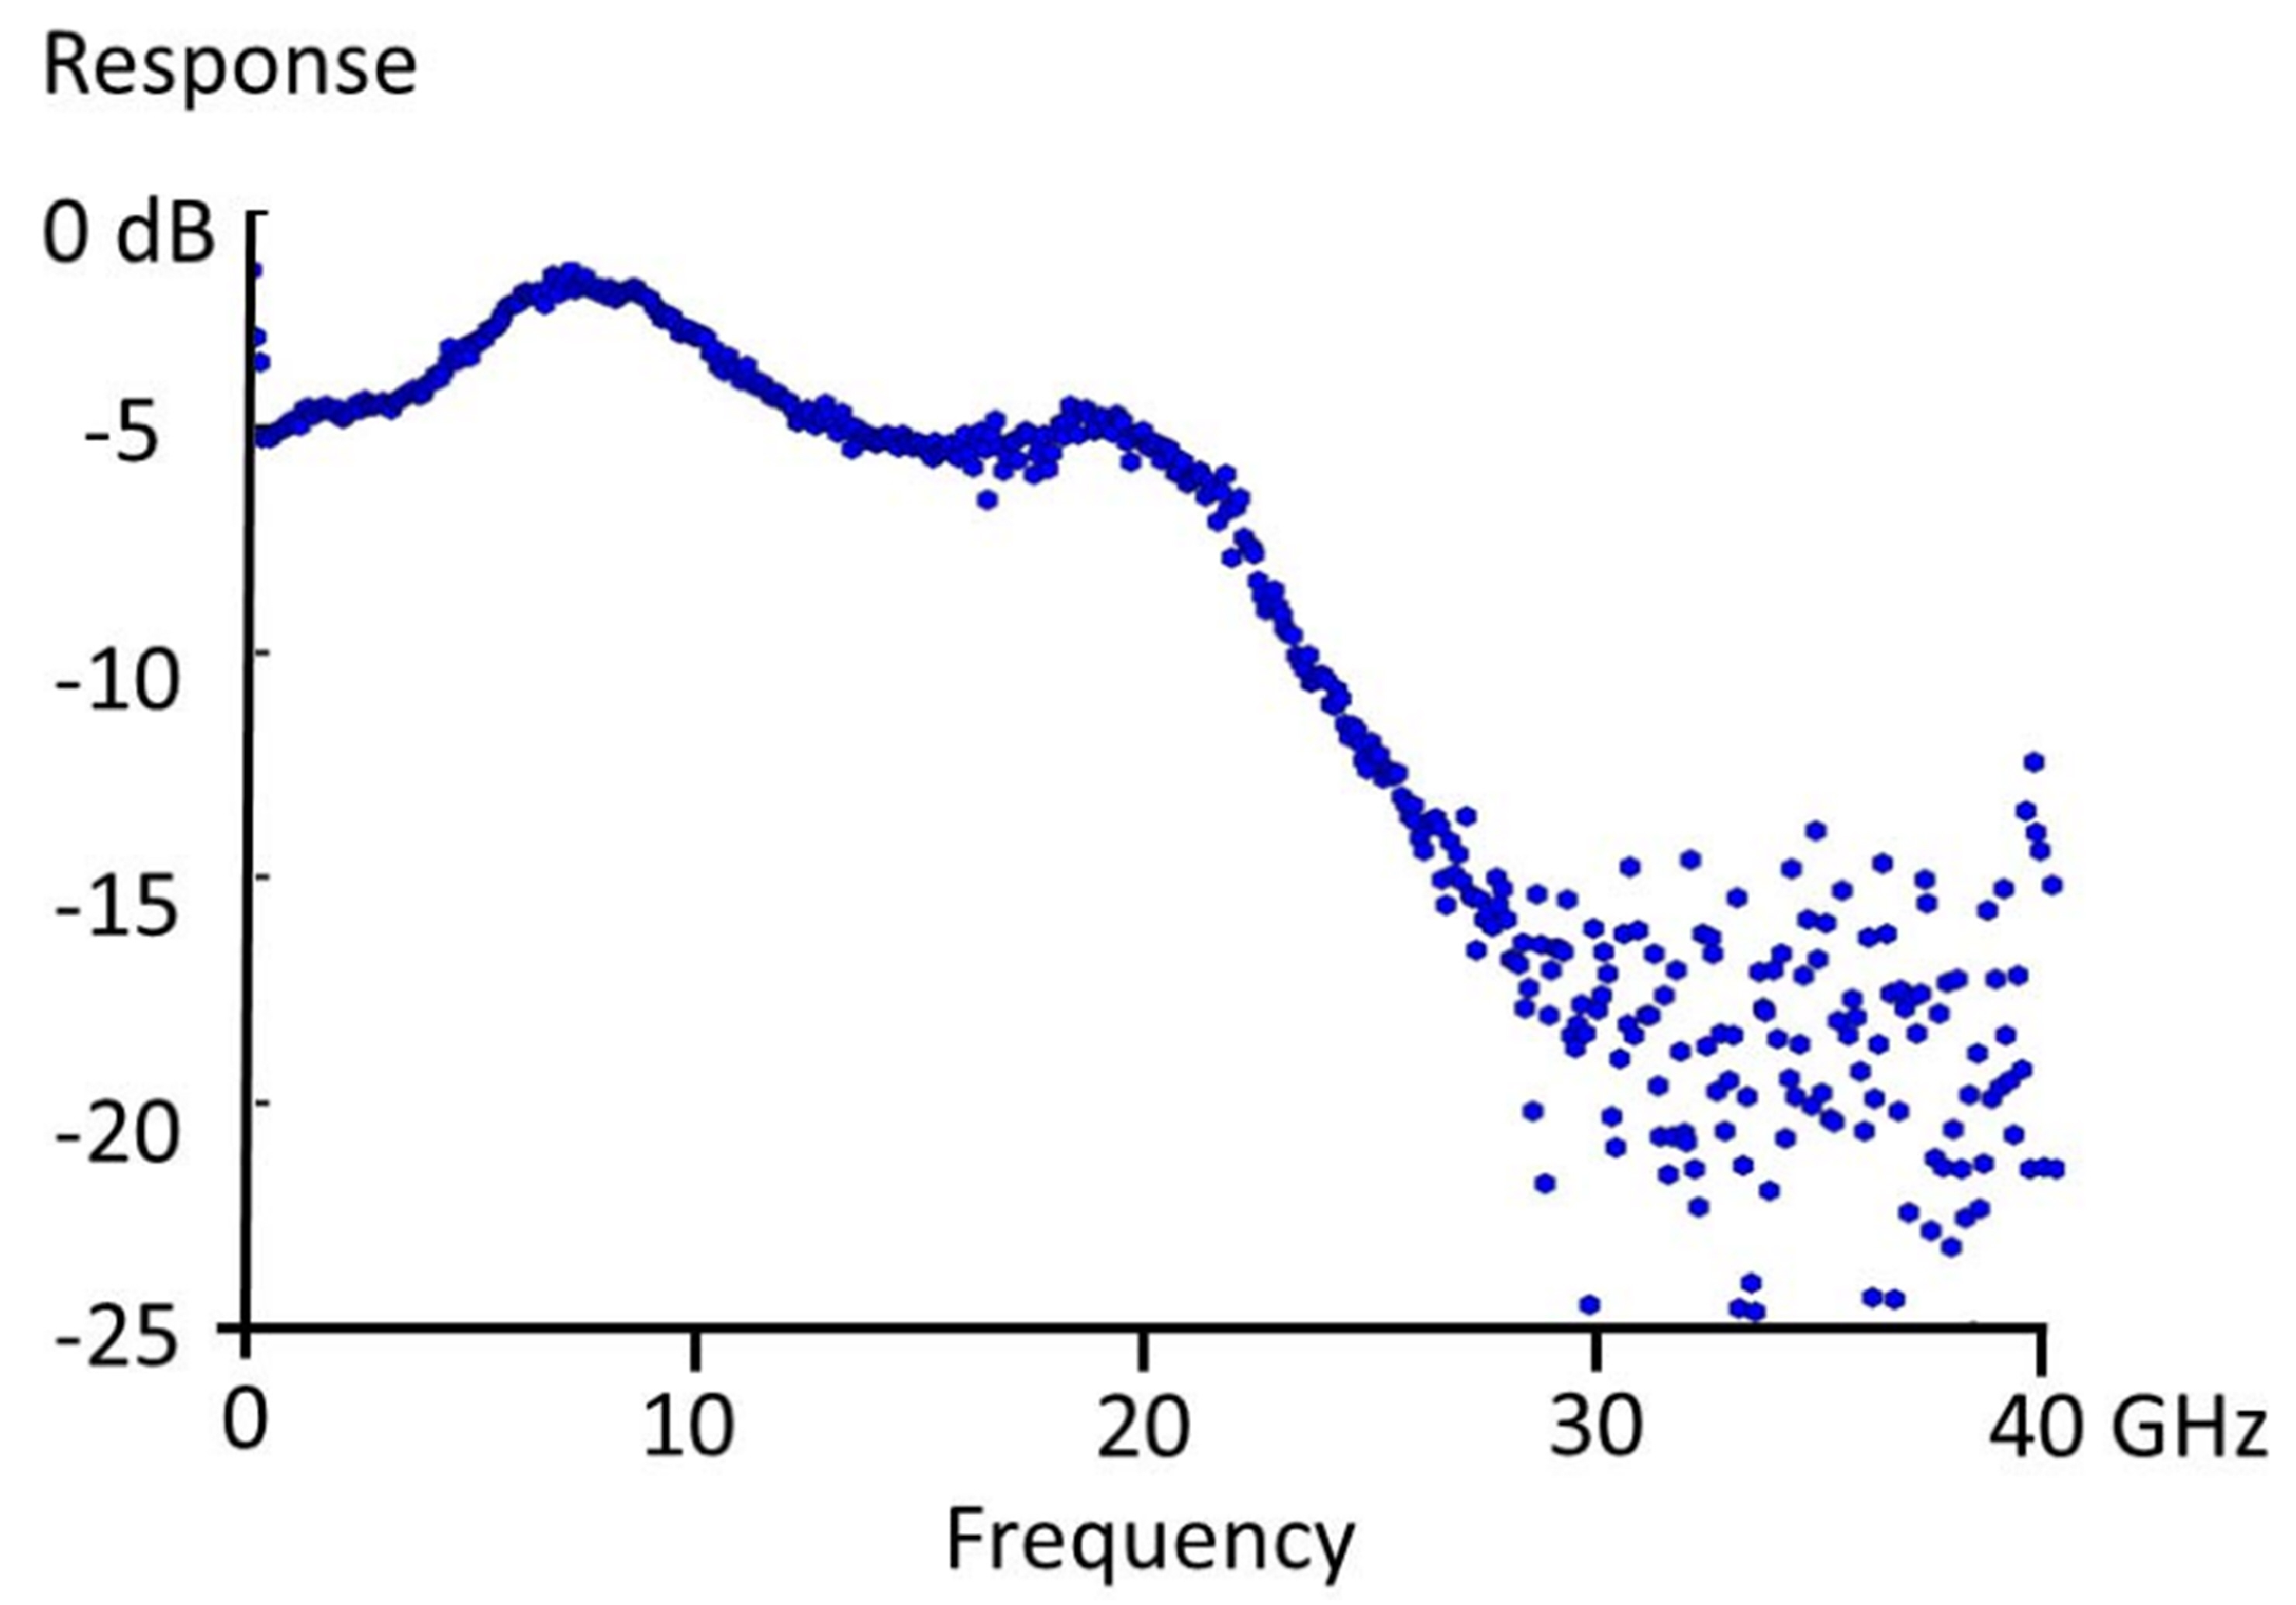
\includegraphics[width=12cm]{./Pictures/laser_s21.jpg}
	\captionsetup{justification=centering}
	\caption{小信号调制响应,I\SB{L}~=~46~$mA$,I\SB{R}~=~60~$mA$\cite{shahin201845}}
	\label{laser_s21}
\end{figure}

我们用来测试激光器调制带宽的实验装置示意图如图\ref{laser_s21_setup}所示,两个数字源表(Keithley 2400)作为电流源来提供自脉冲激光器左右两段的直流偏置。第一个数字源表直接与自脉冲激光器的其中一个电极相连,第二个数字源表通过偏置器(Bias Tee)与从矢量网络分析仪(performance network analyzer, PNA, Keysight PNA-X)发出的微波信号相结合,再通过高速GS探针加载到自脉冲激光器的另一个电极上。被调制后的光通过光纤经掺铒光纤放大器(erbium-doped fiber amplifier, EDFA)放大,输入到高速探测器转换成电信号,生成的电信号输入PNA就可以得到某个调制频率下激光器的响应。通过PNA扫描微波信号的频率,就可以得到激光器的调制响应S\SB{21}曲线。

我们通过扫描自脉冲激光器左右两个电极的泵浦电流组合,得到调制带宽性能最佳的情况如图\ref{laser_s21}所示,此时两个电极的电流分别为I\SB{L}~=~46~$mA$,I\SB{R}~=~50~$mA$。在扫描过程中,当自脉冲频率与驰豫振荡频率相距较远时,我们得到的调制带宽没有明显的提升。从图\ref{laser_s21}的测试结果中我们可以看到,该激光器的驰豫振荡频率在9 GHz附近。除了这个峰以外,在20 GHz附近还有一个光子共振峰,从而使得该激光器的调制带宽达到23~GHz左右。

\subsection{自脉冲激光器的数据传输测试}



得到自脉冲激光器的调制带宽之后,我们需要测试其数据传输的性能。测试装置示意图如图\ref{laser_data_transmission_setup}所示,两个数字源表作为电流源来提供自脉冲激光器左右两段的直流偏置。第一个数字源表直接与自脉冲激光器的一个电极相连,第二个数字源表通过偏置器与来自码型发生器(pulse pattern generator, PPG, SHF 12100B)经微波放大器(SHF S807)放大的的信号相结合结合,加载到激光器的另一个电极上。被调制后的激光器输出经过EDFA放大,经2~$km$非零色散位移光纤传输后用窄带光滤波器滤除EDFA引入的其他波长的光,然后通过一个可调衰减器输入到高速探测器中,探测器将输出的电信号通入数字信号分析仪(digital series analyzer, DSA, Tektronix DSA 8300)就可以得到数据传输的眼图。

\begin{figure}[htb]
	\centering
	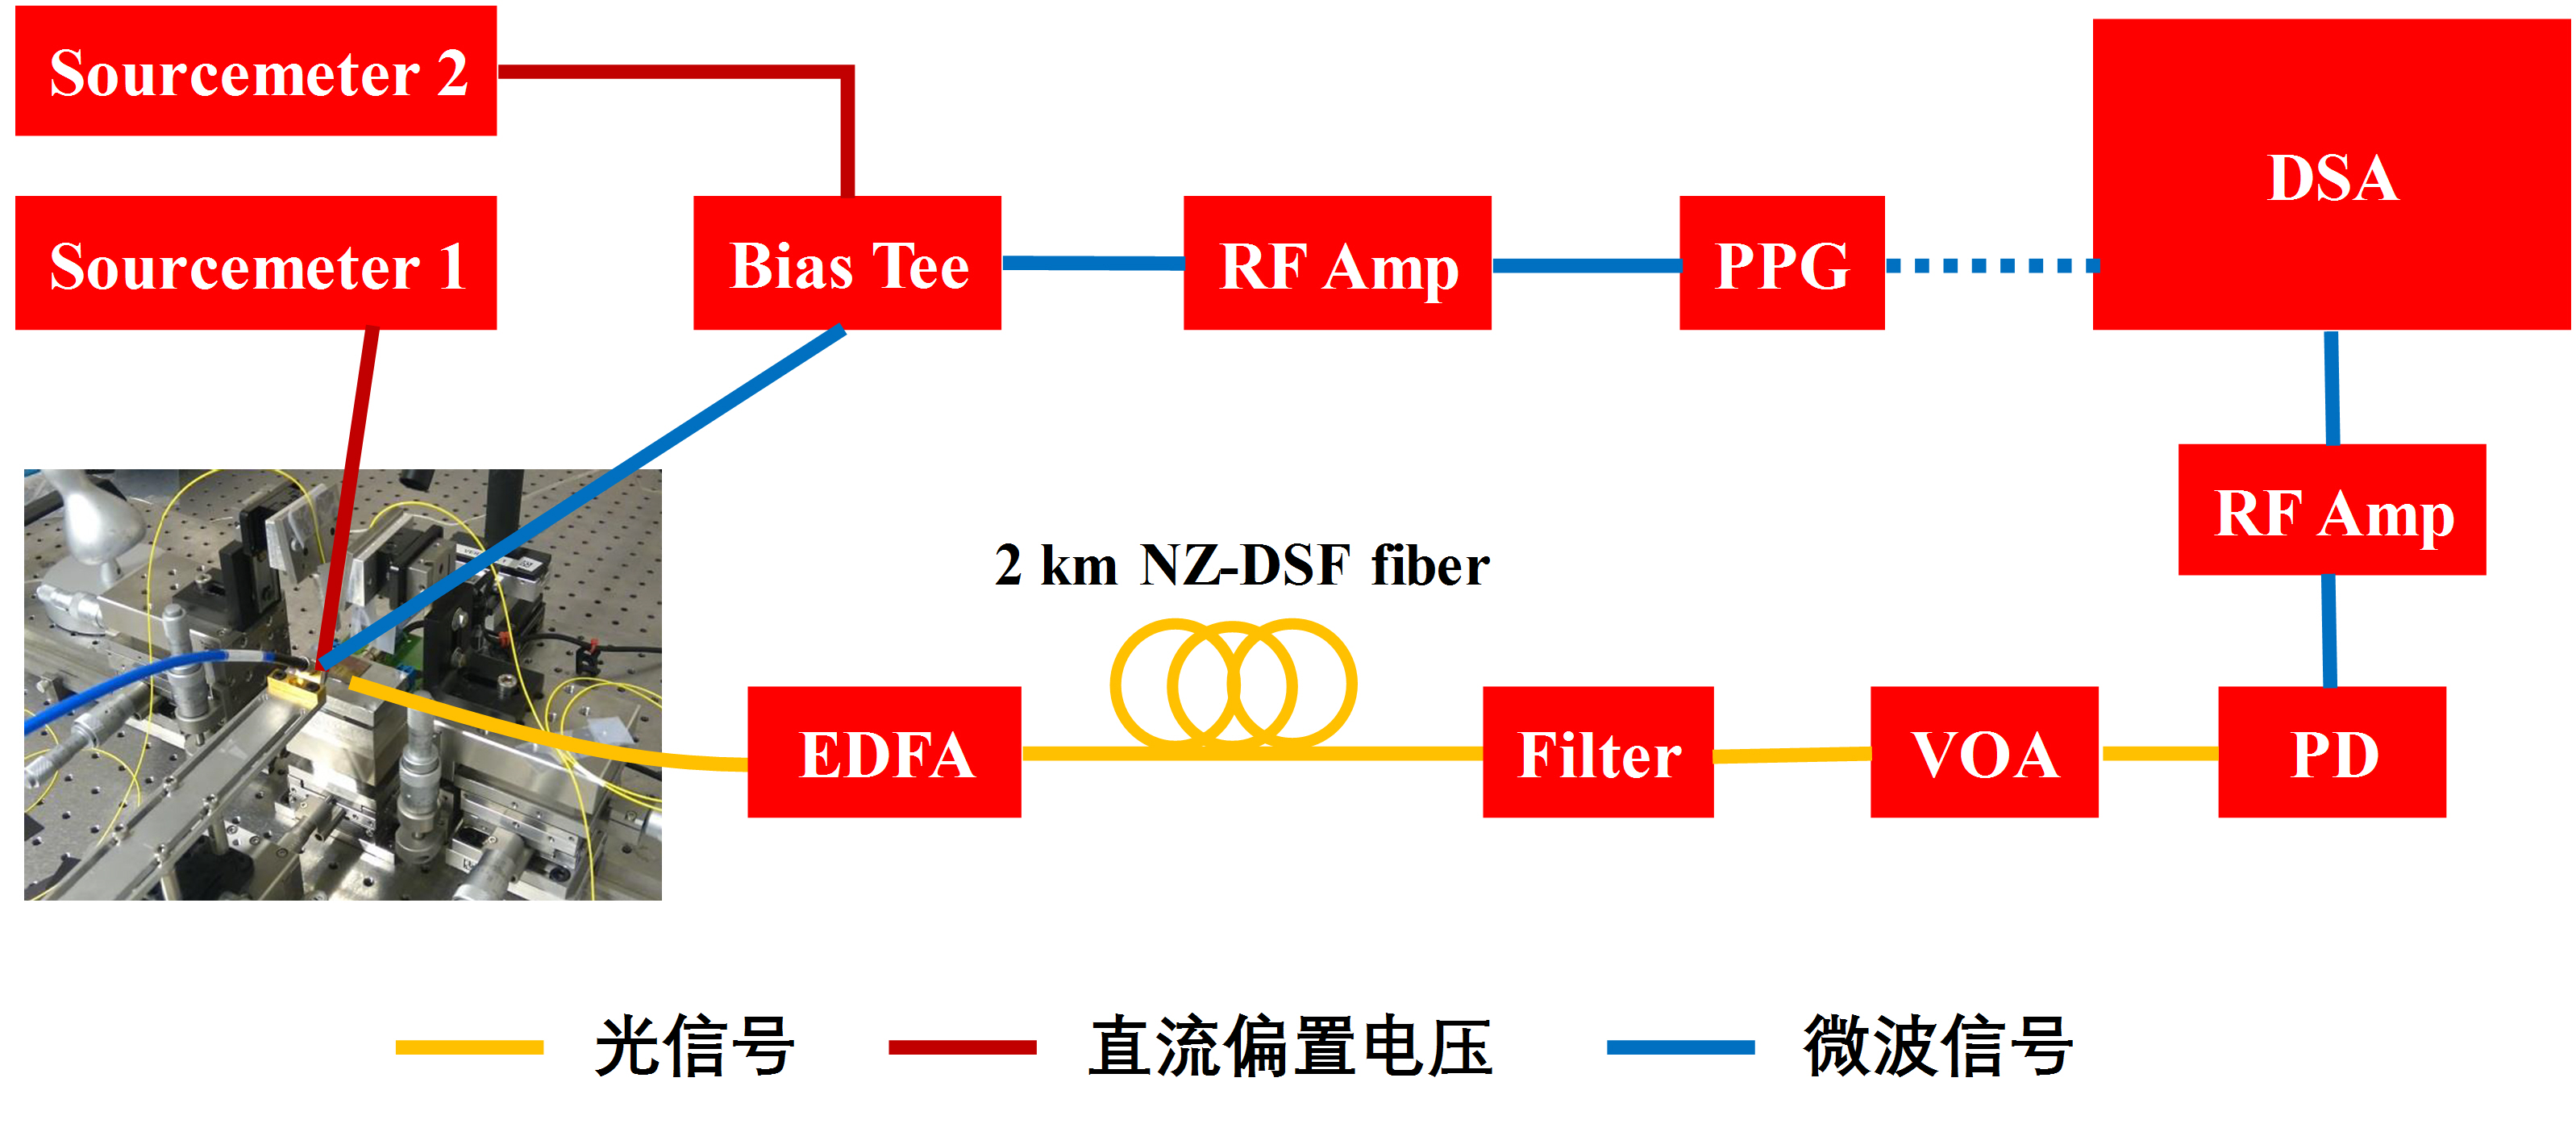
\includegraphics[width=15cm]{./Pictures/laser_data_transmission_setup.jpg}
	\captionsetup{justification=centering}
	\caption{自脉冲激光器数据传输测试示意图}
	\label{laser_data_transmission_setup}
\end{figure}

\begin{figure}[htb]
	\centering
	\includegraphics[width=14cm]{./Pictures/laser_data_transmission.jpg}
	\captionsetup{justification=centering}
	\caption{45 Gbps NRZ数据传输眼图,I\SB{L}~=~46~$mA$,I\SB{R}~=~50~$mA$:(a)背靠背;(b)2 $km$非零色散位移光纤\cite{shahin201845}}
	\label{laser_data_transmission}
\end{figure}

该激光器的数据传输测试工作由Mahmoud帮助完成。PPG产生长度为2\SP{7}-1的非归零码(Non-Return-to-Zero, NRZ)信号,然后通过微波放大器将信号峰峰值V\SB{pp}放大到2.2 $V$,此时自脉冲激光器的左右两电极直流偏置为:I\SB{L}~=~46~$mA$,I\SB{R}~=~50~$mA$,激光器的输出功率为-5 dBm。这与图\ref{laser_s21}得到最大调制带宽时的条件略有不同,因为S\SB{21}曲线只是通过小信号调制大致给出了激光器的调制性能,实际进行数据传输时,需要考虑实际的大信号响应。

当调制速率为45 Gbps时,测试了背靠背与通过2 $km$非零色散位移光纤传输两种情况下的眼图,结果如图\ref{laser_data_transmission}所示,该眼图已经通过一个根升余弦滤波器(root-raised-cosine filter, SRRC)进行滤波,可以看到睁开的眼图。还测试了背靠背与通过2 $km$非零色散位移光纤传输两种情况下误码率与接收功率之间的关系,如图\ref{laser_ber}所示,从中可以看到,对于45 Gbps的传输速率来说,-7 dBm的接收功率就可以满足误码率低于7\%的前向纠错编码开销的硬判决(hard decision forward error correction, HD-FEC)条件。

\begin{figure}[htb]
	\centering
	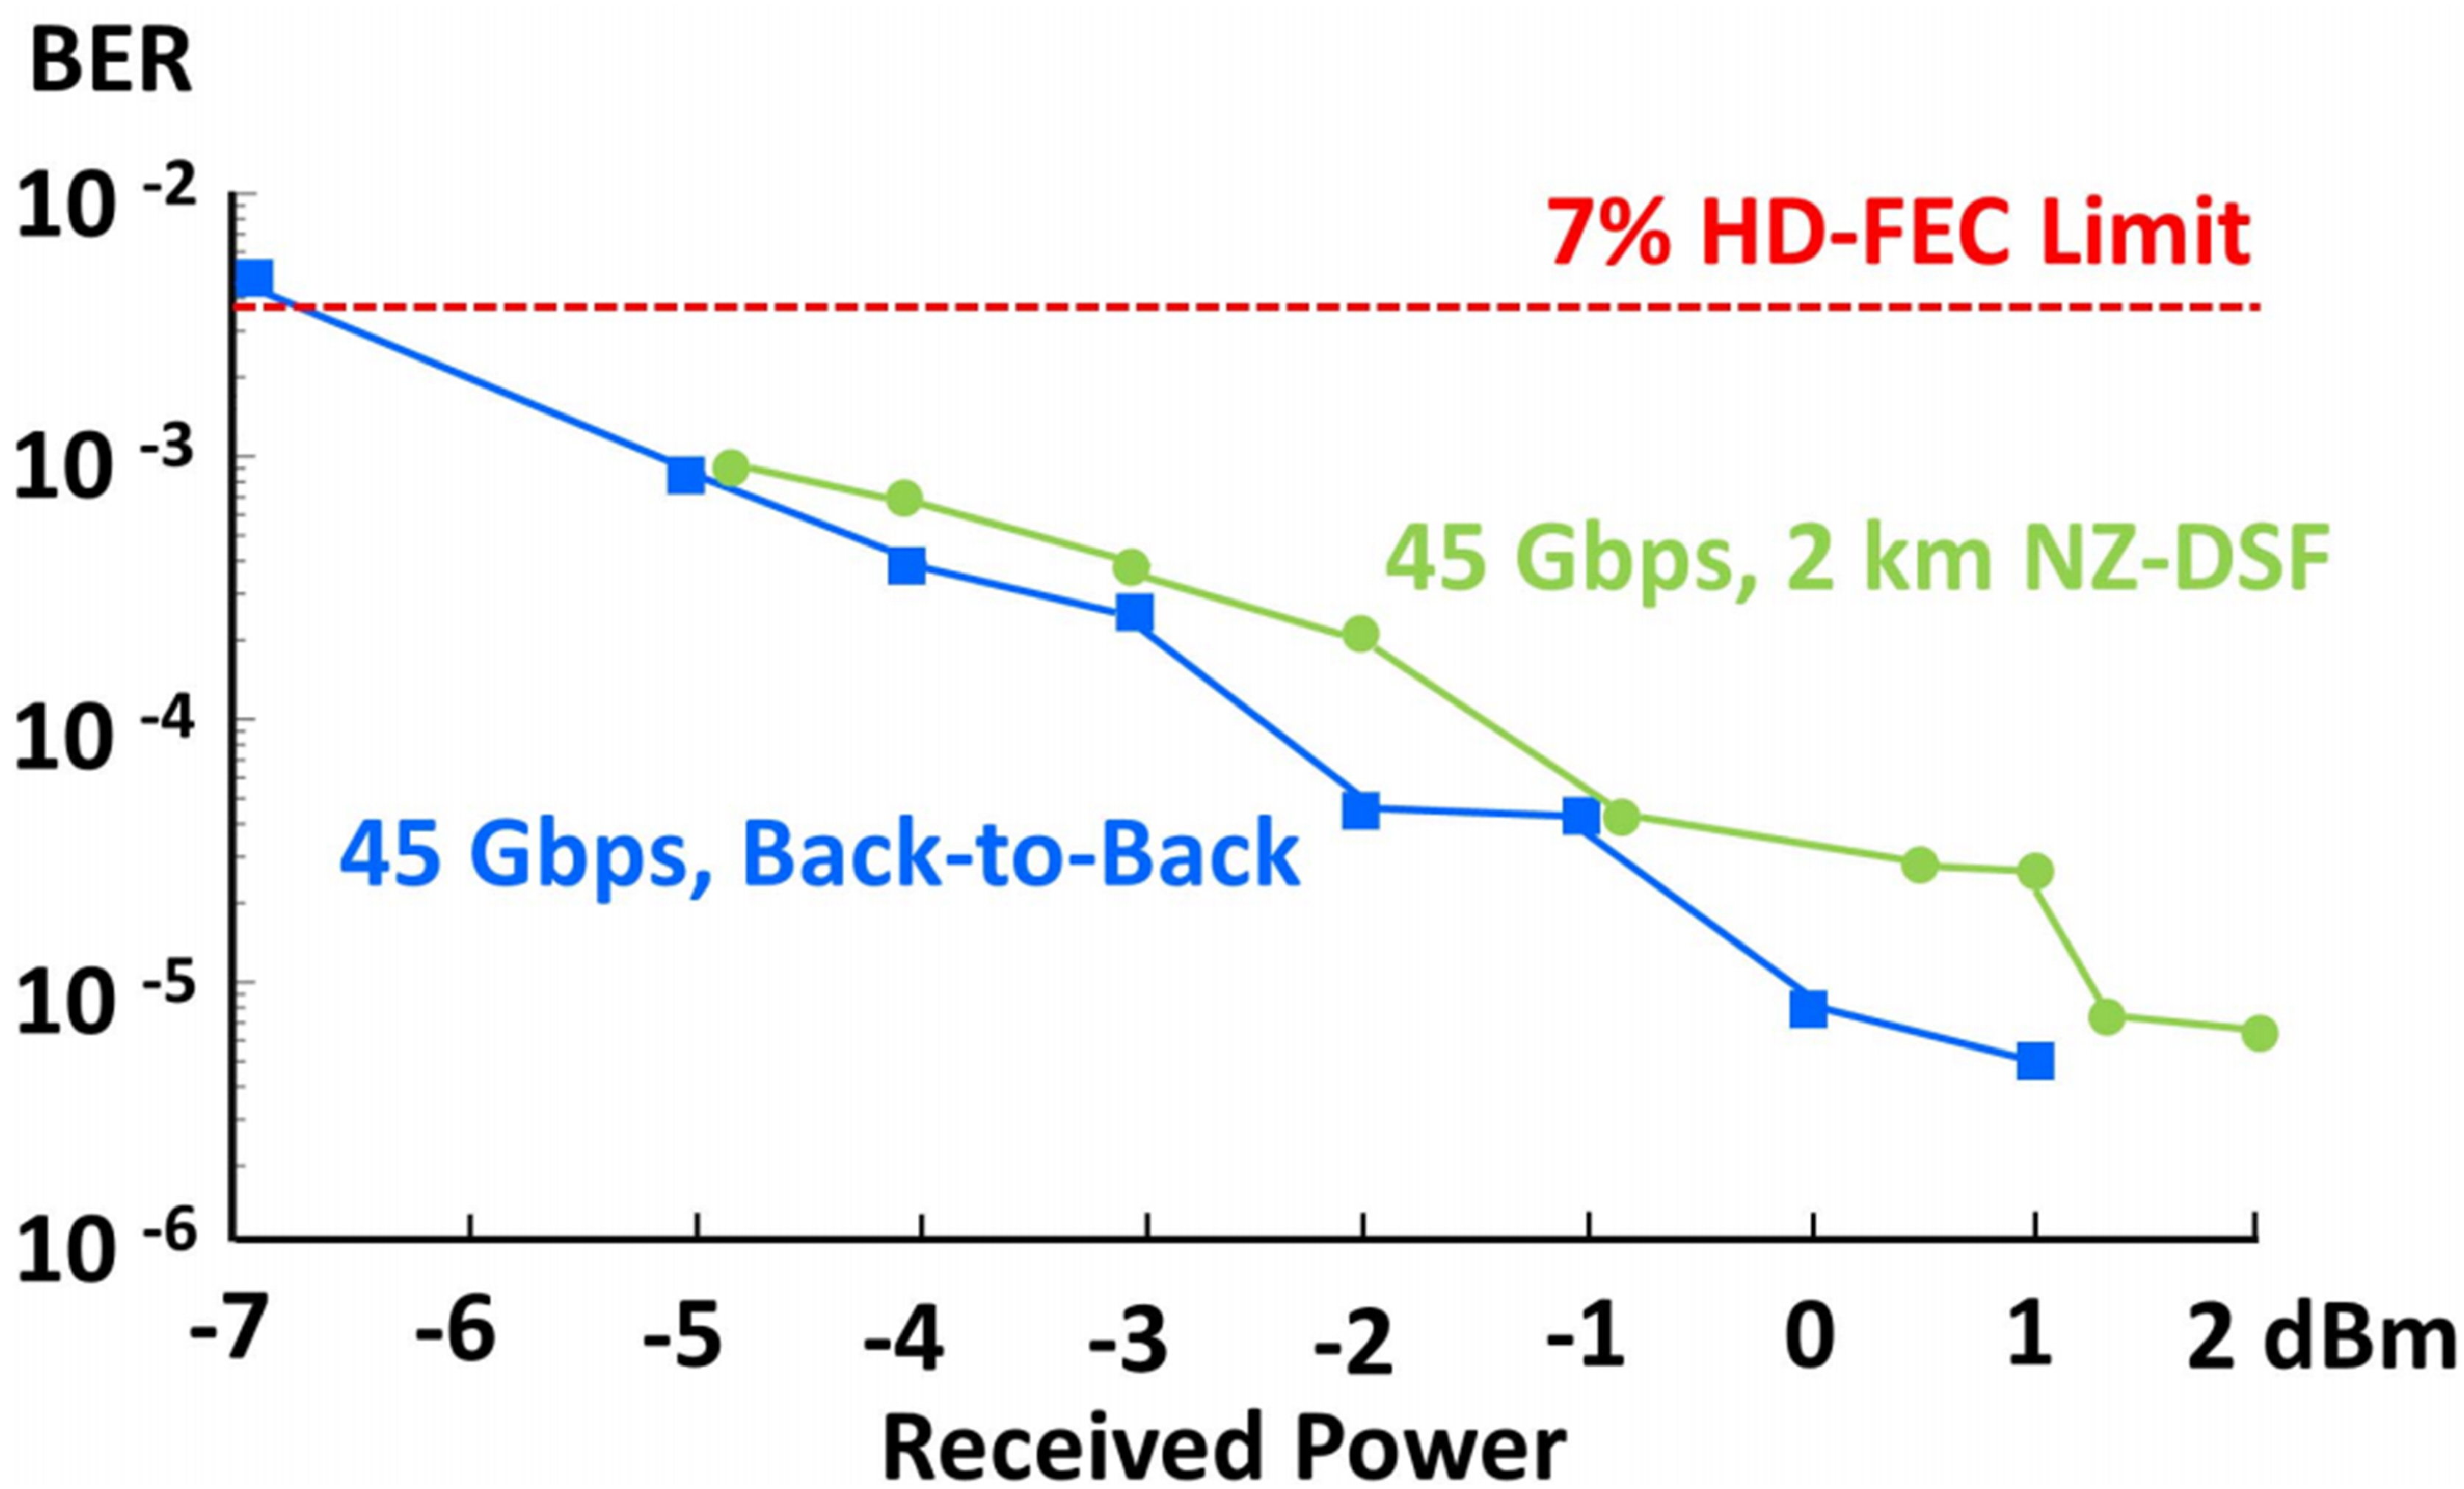
\includegraphics[width=13cm]{./Pictures/laser_ber.jpg}
	\captionsetup{justification=centering}
	\caption{接收功率与误码率之间的关系\cite{shahin201845}}
	\label{laser_ber}
\end{figure}

\section{本章小结}

本章首先介绍了三种实现自脉冲激光器的方法,分析了每个方案的特点。随后提出了一种硅基III-V混合集成的双段式自脉冲DFB激光器。然后介绍了硅基III-V混合集成的实现方法,并设计了一系列基于一阶光栅的双段式DFB激光器,它们有不同的III-V波导长度,两端通过锥形波导结构与SOI波导进行垂直耦合。随后,详细介绍了该器件的制作工艺流程。器件制作完成之后,先用电压快速退火的方法对每个激光器的电极进行快速退火,然后测试了其IV与PI曲线,得到激光器的阈值电流在12~$mA$左右。通过大量的实验数据,发现了激光器长度与产生自脉冲信号之间一个有趣的现象。之后研究了自脉冲信号频率与左右两段激光器泵浦电流和温度的关系,再之后研究了自脉冲信号的频率锁定现象,通过该方法,可以实现线宽小于10~Hz的光学微波信号。最后验证了自脉冲激光器可以通过光子共振现象来提升激光器的直调带宽到23 GHz左右,并实现了45 Gbps的直接调制数据传输速率。


